
\documentclass[12pt,reqno]{report}      % Sets 12pt font, equation numbers on right
\usepackage{amsmath,amssymb,amsfonts} % Typical maths resource packages
\usepackage{graphics}                 % Packages to allow inclusion of graphics
\usepackage{color}                    % For creating coloured text and background
\usepackage{siunitx}                  % for degrees celsius
\usepackage[toc,page]{appendix}
%\usepackage[margin=2in]{geometry}
\usepackage{lscape}
\usepackage{float}


\usepackage[colorlinks,citecolor=blue,linkcolor=blue]{hyperref}                 % For creating hyperlinks in cross references. It should be after the color package. The option colorlinks produces colored entries without boxes. The option citecolor=blue changes the default green citations to blue.
\renewcommand{\theequation}{\thechapter.\arabic{equation}}

\DeclareGraphicsExtensions{.pdf}
\parindent 0cm
\parskip 0.2cm
\topmargin 0.2cm
\oddsidemargin 1cm
\evensidemargin 0.5cm
\textwidth 15cm
\textheight 21cm
\newtheorem{theorem}{Theorem}[section]
\newtheorem{proposition}[theorem]{Proposition}
\newtheorem{corollary}[theorem]{Corollary}
\newtheorem{lemma}[theorem]{Lemma}
\newtheorem{remark}[theorem]{Remark}
\newtheorem{definition}[theorem]{Definition}

\makeatletter
\def\thickhline{%
  \noalign{\ifnum0=`}\fi\hrule \@height \thickarrayrulewidth \futurelet
   \reserved@a\@xthickhline}
\def\@xthickhline{\ifx\reserved@a\thickhline
               \vskip\doublerulesep
               \vskip-\thickarrayrulewidth
             \fi
      \ifnum0=`{\fi}}
\makeatother

\newlength{\thickarrayrulewidth}
\setlength{\thickarrayrulewidth}{4\arrayrulewidth}


\def\W{$\mathbb{ W}$}
\def\R{\mathbb{ R}}
\def\S{\mathbb{ S}}
\def\I{\mathbb{ I}}
\makeindex


\title{Mbona Private Nature Reserve \\
        Trout Hatchery \\
       % \vspace{2cm} 
        %Mbona Fishing Committee \\
        \vspace{2cm}
        \today}

\author{
\htmladdnormallink           % Puts a hyperlink on to the author's name
{Hugh Murrell}{http://www.cs.ukzn.ac.za/~hughm}, Editor \\
\htmladdnormallink
{Pierre Olivier}{http://www.pierrecraft.co.za}, Technical \\ \\ \\
with a foreward by: \\
\htmladdnormallink
{Dennis Dyer}{http://www.mbona.co.za}, Chairman \\  
\vspace{1cm} \\
{\small\em \copyright none at all }}

 \date{ }
     \usepackage{draftwatermark}                   %%%   These four lines
      \SetWatermarkText{}   %%%   put a watermark
       \SetWatermarkScale{3}                          %%%  on all pages. Just omit them if 
        \SetWatermarkColor[rgb]{0.9,0,0}               %%%  it is not needed.
\begin{document}
\makeatletter\@openrightfalse
\maketitle
 \addcontentsline{toc}{chapter}{Contents}
\pagenumbering{roman}
\tableofcontents
\listoffigures
\listoftables


\chapter*{Preface}\normalsize
  \addcontentsline{toc}{chapter}{Preface}
\pagestyle{plain}

This manual is a basic guide to the running of a successful practice of 
small-scale trout farming. It summarises all the technical information that is 
important to know for small-scale trout production.

This document was created using 
{\htmladdnormallink {Leslie Lamport's}{ https://en.wikipedia.org/wiki/Leslie_Lamport}} document preparation system \LaTeX \cite{lamport}.
The content for the first chapter of this manual was mostly copied from a document  called {\it Small-scale rainbow trout farming} issued by 
the Food and Agriculture Organisation of the United Nations \cite{fao} which has been placed in
the public domain at 
{\htmladdnormallink{http://www.fao.org/docrep/015/i2125e/i2125e.pdf}{http://www.fao.org/docrep/015/i2125e/i2125e.pdf}} This {\bf fao} document has a copyright notice that encourages reproduction and dissemination of the material it contains with a statement that non-commercial uses will be authorized free of charge on request. 

In later chapters, this FAO document is augmented using the local knowledge of:

\begin{itemize}
  \item[] {\bf Dave Forsyth}, Mbona Manager, 2016-Present
  \item[] {\bf Guy Reen}, Mbona Assistant Manager, 2018-Present
   \item[] {\bf Gareth Powell},  Mbona Conservation Officer, 2000-2018
  \item[] {\bf Gavin Chin}, retired Trout Hatchery manager.
\end{itemize}
  
Editing and oversight of this document was carried out by:
\begin{itemize}
\item[] {\bf Dr. Dennis Dyer}, Mbona fishing committee chairman, 2000-Present
\item[]  {\bf Bernard McDonald}, Local fisherman, historian and linguist.
\end{itemize}

The purpose of this manual is to guide the reader through the necessary technical information, 
and practical solutions to the day-to-day operation of a small-scale Rainbow Trout farm with
particular emphasis on the infrastructure setup and operating procedures at the Mbona Hatcheries.

\chapter*{Foreward}\normalsize
  \addcontentsline{toc}{chapter}{Foreward (by Dennis Dyer)}
\pagestyle{plain}

Awesome Mbona! We, members of the Mbona Family, which extends over 50 years, 
have so much to be grateful and thankful for to a special few, headed up by Eric and Pat MacKenzie. 
What a profound vision they conceptualised, to build the paradise that we have all shared. 
Mbona has had a huge effect on our families and our children who have been able to free themselves 
of fear and many restrictions that have become a way of life in our country.
It is my pleasure and privilege to capture for you the history of trout and fishing as an additional recreation 
available to us on Mbona.

It all started one sunny day in late 1973 as Eric MacKenzie was walking close by the Crystal stream 
accompanied by a friend Edward Austin. Eric asked if there were any signs of fish in the area, 
Edward?s response was to catch a grasshopper and toss it into the stream. 
Almost instantaneously there was a swirl on the surface and the grasshopper was history, 
yes history in the making of trout fishing available to us. 

Such a simple beginning to a sport that has given so much joy to many.
Dams were mapped and designed with details of location demarcated. 
Drummond and Michael MacKenzie were tasked with naming each dam, 
they came up with the names that have become so familiar to us over the years, 
each having a special place in the hearts of enthusiastic anglers. 

They are:  Crystal, Rainbow, Laughter, Amber, Pateric, Emerald, Deep Pool, Evergreen and Holbeck. 
The list was sent to Pat and Eric, who were most impressed with the names. 
Pat was puzzled by the name which she pronounced Paterric for a short time until 
the penny dropped and she and Eric are forever remembered by the special name of this dam.

Today, it is so easy to name the dams, choose where we would like to fish and go 
and enjoy an experience that includes a magnificent environment, peace and quiet, birds, buck 
and occasional greetings to other shareholders as they walk or ride the many routes offered in our paradise. 
What we do not appreciate is the mammoth task that was undertaken to create these facilities. 
Crystal has a dam wall that is over 200meters long, how much earth works was needed is 
mind boggling and the cost in today's standards would make it prohibitive to build. 
Each dam has been skilfully engineered and apart from Emerald, 
which has an irreparable leak, are functional all the year around.

% \subsection*{The Dams}

Some facts about Mbona dams:

\subsubsection*{Crystal,  21 hectares, 52 acres Completed in December 1972.}

Crystal is our largest dam. In the late 1976 a major rain storm occurred in and around Mbona. 
This resulted in a neighbouring dam above Evergreen, which had Bass in it, to overflow into Evergreen 
and to introduce Bass into its waters. It was decided to drain Evergreen which at that time was 
successful in getting rid of the Bass. Evergreen communicates with Crystal and the bass arrived 
and multiplied at a significant rate. The problem of the Bass in Crystal was the subject of much concern and debate. 
Draining of Crystal was not a consideration. After some time Bass were again seen in Evergreen. 
Today the consensus opinion within the Fishing Subcommittee is to rather create another facility for 
recreation so we have opened Crystal to a limited Bass fishing opportunity. 
Bass fishing is allowed with fixed spool reels and single hooked lures. Catch and keep is what is encouraged. 
This in fact has been a great boon to younger children, who now spend hours trying to catch bass and Bluegill 
which have also proliferated in Crystal. There have been no complaints received and in fact there have 
been a number of Bass caught between 3.5 and 5kg. Trout are caught in Crystal and one?s impression 
is that these numbers are on the increase which we believe is due to a more aggressive stocking program. 
Over the years there has been reference to concerns about reed encroachment in the southern end or inflow area between 
Laughter and Crystal. This is being discussed again, although it is a daunting task to dredge the area because 
silting up is the problem with the reeds flourishing in the enriched shallow water. 
There are discussions re creating a small wetland between Laughter and Crystal.

\subsubsection*{Evergreen,  10 acres. Completed 1975.}

Referred to above is the Bass problem in Evergreen and the floods in 1976. As noted Evergreen was drained 
and Bass exterminated, this was successfully done with people being asked to get rid of Bass by taking them 
home and trout were netted and transferred to Crystal.  Bass were back in Evergreen shortly after damage to 
the communication channel between Evergreen and Crystal had occurred. This was thought to be due to the 
fact that the Bass were able to swim up the damaged runway. Evergreen also had a problem with weed overgrowth 
and Grass Carp were introduced with good effect. There are no records relating to this, however, despite 
the fact that Grass Carp are supposed to concentrate their efforts on the periphery, the end result was positive. 
Of interest is that at one stage off Ernie?s walk, that circumvents Evergreen, a viewing platform was constructed 
5 meters above the water from which one could watch the fish swimming in the shallows. 
Grass Carp are now classed as exotic and it is virtually impossible to get hold of. Evergreen is a popular dam 
with floating tubes allowed, there are reports of excellent catches including some 3.5 kg bass. 
For some years it  was a catch and release dam, the fishing Committee at that time expressed their satisfaction 
with the outcome of this, however, other fishermen had had years of happy catching and preparing for the 
table and the decision to release has been recently lifted. If only our returns were more reliable, 
we could make a better than guessing as to the results.

\subsubsection*{Amber, 1 acre and Pateric, 2.5 acres, were both completed in 1973}

These two dams have regular reports of good catches. The recent blockage of the outlet from Pateric to Amber 
has been cleared and Amber has been overflowing for a good part of the year. Pateric has had leaks 
repaired on a number of occasions, however, every winter during the dry season, there is a significant drop in its level. 
A definite observation is that this dam is one of the most productive for catching trout and there is speculation that 
the nutrients available are due to enhanced growth of foliage during the low level periods.
Over the years Amber has produced a number of surprises of Rainbows over 2.5kg and a lone Brown of 2.2kg, 
this fish was returned to the water in good condition.

\subsubsection*{Rainbow: 3.2 acres, Laughter 4.2 acres, Deep Pool .75 acre and Holbeck 0.25 were all completed before the end of 1975.}

Rainbow has also had its catch and release restriction lifted, it is a very popular productive dam with a recent report of a 
2.5kg Brown caught and released.
Laughter has produced its share of excitement over the years. During the recent past there are no reports of Bass in this dam, 
although Bluegill are reported intermittently, however, 5 and 8 years ago there were Bass in Laughter. In both cases Laughter 
was drained and we have successfully rid  them of bass. There are a number of hypotheses mooted to explain this as there is 
no source of water that could be blamed as the source of the contamination. This included the possibility of fertile eggs attaching 
to the legs of water birds whilst visiting Crystal and then being transferred to Laughter. Our thoughts were more directed to 
suspect some human mischief. Since the last drainage, we have had no reports of Bass.
Each dam is unique and has a special attraction for a number of different fishermen. Both Holbeck and Deep Pool have been 
productive happy places for many of our shareholders. Holbeck is posing a problem with having silted up considerably. 
There are two camps, one wanting it to be left alone and the other hoping to dredge it and return it to its glory as a popular spot.

\subsubsection*{The Hatchery}

The dams were eventually completed and we had the waters within which we could pursue our desire to enjoy fly fish for trout on Mbona.
The next step was to tackle the project of locating a source for trout, this led to the need to get in expert advice and guidance. 
This required a well thought out plan taking into consideration all the unique elements pertinent to Mbona. 
It was obvious that this was not just going to be an occurrence. It was going to be a long process that needed 
conscientious dedicated people to drive and maintain it. 
It needed financing and the blessing of the Joint Board of Directors who would support it financially and allow access to 
the permanent staff. This management team needed to be replicated as time went on and as the Board changed new 
people were needed to get involved. Throughout our history, we have had these people, 
many of them giving significant input of time and expertise. 

In December of 1973, the first joint board AGMeeting occurred. It was at this meeting that guidance from Terry Oatley 
was sought with respect to trout fishing at Mbona. Terry Oatley was a member of the Natal Parks Board and fortuitously 
was a shareholder at Mbona and this was one of his many contributions.
It was concluded that the location of Mbona, its elevation and its Climate would at best leave us with a situation that 
was marginal in our quest for creating a successful sporting and recreational facility 
for any of our interested shareholders. The initial decision was to stock our dams with 10inch fish. 
This was thought to be the most viable size to allow for optimal survival against weather conditions, predators such as otters, 
fish eagles and cormorants, the numbers of trout stocked in each dam was carefully worked out according to the volume of water 
in each facility, this is still being used as a guide today. Using Terry?s contacts, the Natal Parks Board documented a plan for Mbona. 
It was soon realised that the transport of the larger fish became a major operation which was both expensive and risky with 
quite a high mortality rate. The decision was made to buy 3000 6-7inch trout which had been calculated as a reasonable amount 
to stock our dams and support the fishing demands.

This meant that a facility needed to be built as rearing tanks for the fingerlings to grow them to the ideal stocking size of about 10inches. 
The basic plan was drawn up and this plan has evolved over the years to our present adequate and efficient system. 
There is a gravitational water supply from Lake Crystal to the ponds, which has had to be modified over the years. 
Some of the points are worth mentioning. We have developed this supply over the past 15 years so that it retains its original 
gravitational principle but so that it is adequate, we have created a dual system. This fulfils two essential functions, an adequate supply, 
which is at an appropriate depth to access the lowest water temperature, without being at too much risk of clogging up with 
debris and secondly is to have an adequate back up system. The fact is that the supply has been interrupted at least twice 
in the past with devastating results of wiping out the whole stock in the ponds. We have a rotational system in place where the inlets 
to these water supplies are checked regularly as part of our maintenance program. The quality of the water is enhanced by passing 
it through our aeration tower, which has also been modified at regular intervals. The new system also gives us the choice of 
increasing our water flow through the system, which is needed in the hotter months. We therefore have a quality, 
reliable and self-powered system which will be described in detail in the chapters that follow.

\subsubsection*{Record Keeping}

One of the most significant developments in the last 10 years is the weighing and counting of the trout at the various stages of 
their lives in the hatchery. The handling has been perfected as are the methods of moving them from the ponds into the 
transporting vehicle, which is fitted with a tank that is well aerated and can accommodate 200 10 inch fish. 
This has allowed us to stock our own dams and deliver to customers, fish that are not compromised and mostly 
don?t even need any resuscitating. This is in contrast to previous efforts that always had a mortality rate. 
We have ensured a process that allows us to accurately size the fish for customers and also for record 
purposes of what is stocked and where.

 Record keeping of expenses has improved, accurate graphs on growth rate and feeding volumes is being 
 more accurately developed and maintained which will allow us to continue improving our production and 
 performance functionally and economically.
 
 The age old problem of monitoring once the fish have left the hatchery continues unabated. 
 From the beginning it was recognised the importance of outcomes of our efforts, fish returns, numbers of 
fishermen, the impact of catch and release initially and further down the line, 
the introduction of float-tubes and allowing them access now to Laughter as well as Crystal and Evergreen. 
Without this data, we will continue to make uneducated guesses rather than produce facts.

From the outset, fish returns have been notoriously poor. There have been a number of unsuccessful schemes, 
including sending a form with the monthly accounts to every shareholder. Apart from the new electronic accounts system 
introduced, this was not a success. Returns to the clubhouse, or the gate on leaving and now by email or on to the website 
are still poorly supported, we would appreciate any suggestions to add a catalyst to this process. 
The truth is, we are not able to assess the success of what we have done without appropriate data.


\subsubsection*{Predators}
What has been shared is the development of the facility over the years to accommodate decisions made as part of the journey. 
To conclude this aspect, the original plan was well thought out and has not changed much, including the pitfalls to a perfect system. 
There have been a number of threats, apart from physical resource maintenance and development. 
The fish are vulnerable to predators even in the confines of the hatchery, shade cloth and nets are there to protect from birds, 
an electrified fence has been the most effective deterrent against otters, although the fence itself still needs attention to its strength. 
We still have a real, although mysterious reduction in numbers of fish from the raceway. It is our suspicion 
that there may be a human element to this phenomenon and the next step is to monitor by camera more frequently. 

\subsubsection*{Acknowledgements}

As previously mentioned, the process was made possible by enthusiastic and interested individuals from conception 
to where we are today. Sharing with those involved, the success is always affected by the attitude of the joint board, 
the availability of funds, the management and the support of the trout and fishing committee. 
Over the years, we have been blessed by having these people to contribute to what we have today. 
A common thread commenting on the support and expertise of different managers every step of the way is 
evident and the present situation is better than any of us have experienced previously.

What a long exciting and productive journey this has been spanning fifty years. 
At the risk of not mentioning all the contributors to the epic, people who have been involved and made 
contributions are included as we summarise the progress over the years. Kindly accept apologies for any omissions. 

To Eric and Pat for their vision and the creation of the vast and superb infrastructure, including the dams, 
their beauty and their accessibility, the MacKenzie clan as well are the founders and to whom we will all be eternally enriched and grateful.

Over the years we need to acknowledge the invaluable support and contribution made by the respective Joint Board members. 
The services of managers, without exception, has been remarkable and appreciated by the trout committees. 
The original plan was researched by Ted Oatley, who used his contacts with the Natal Parks Board to produce a detailed assessment 
of the situation and then put together a plan of action. The basics of that plan are still being used today. 
We are in a process and this plan has been modified and developed to suit the needs of each successive committee.

The initial phase was to create the hatchery with the water supply from Crystal. The aerator was built, the three ponds created 
which were originally made of corrugated iron and the raceway. Garth Hatton was the first trout committee chairman. 
His services extended over the next 15 years, he has made a fantastic contribution over these years and was 
faced with many problems and also contributed to modifying the original plans to improve, not only the physical resources, 
but also the quality of the actual fishing. 

During his time he faced many challenges which included making the hatchery safer from predators, 
draining of Evergreen to get rid of the bass, increasing the capacity of the ponds as well as converting the ponds to brick and mortar, 
he rebuilt the aeration tower and produced a number of comprehensive reports which related to quality of the water in the dams, 
fishing rules and advice on stocking. He was well supported by the board and particularly the managers.

Chairmen that followed were among others, Richard Erasmus and Ken Cohen who was followed by 
first Nick and then Charles Shave who together served for more than 10 years up until 2005. 
All these men made every effort to maintain and improve conditions, each one has faced challenges including 
some disasters where large numbers of fish died. 
This was due to water supply failure, inclement weather conditions, otter invasions and even a few incidents of poaching. 
They were party to the decision to create catch and release restrictions in Rainbow and Evergreen, 
they retained the sourcing, purchasing and growing the trout, they were responsible for maintaining the hatchery 
and for seeing that the dams were properly stocked. They were continually devoted to improving the fishing as a quality recreation.

During the years, we have had expert advice and input from well known and respected trout fundies particularly 
Rob Karssing and Jake Alletson are acknowledged and thanked.

The present committee has been functional since 2005. They have faced all the problems of their predecessors 
including episodes of losses due to water blockages, maintenance of the hatchery and trying in vain to 
get better records of number of fishermen and their catches. An important decision was taken to buy trout eggs 
instead of buying fingerlings of 6 inches. This decision was taken in 2012 and it has changed our process 
considerably and has allowed us to increase our numbers substantially. The resources have been documented 
earlier in this article as well as the process of rearing the trout through the various phases of development. 
The venture has been successful.  We researched the process carefully and introduced scientific measures to 
measure temperature and oxygen content in the water accurately. 

We have improved the management of moving of trout and have got this down to a fine art. 
There has also been an improvement in all record keeping both monitoring growth and general running costs. 
The driving principle was to improve the fishing at Mbona primarily and secondly to sell fish of 30cms in size to neighbouring facilities. 
This has proved quite successful and we will continue to have frequent meetings, hoping to improve all of our ventures. 
We also took the decision to open Crystal to limited bass fishing as previously mentioned and to allow floating tubes on Laughter. 
The latter decision resulted in an exciting afternoon?s fishing producing over 20 nice sized fish. 
The committee is very active and meets regularly and would welcome new members, especially some younger enthusiasts.

There are a number of issues that we would really appreciate help with and suggestions one of  these is record keeping, despite the website facility, still leaves much to be desired. This is so important for us to know whether we are being successful or not and will guide in future plans. The Easter and Christmas fishing competitions are not as well supported as we would like. We are planning to supply trout to shareholders by an ordering system and would like to hear whether there is enough of a demand for them.

In conclusion, all previous contributors to this facility are to be saluted and thanked. 
The present committee has been active since 2005. It has been a great journey together of enthusiastic members 
doing research and development. This has been a shared experience. Each member has brought to the 
committee something special and all have been willing to attend meetings and especially to carry out tasks that they have undertaken to do. 

Jacko Jackson brought a wealth of scientific know how and expertise, 

Pierre Olivier has been a tower of strength with his practical experience and unrelenting service of maintenance, 
development and even deliveries is invaluable. 

Bernard McDonald always willing, contributed much knowledge and was always prepared to be hands on. 

Pete Barbour was our marketer and has established a nice clientele which has now been taken over by Ronnie Ritchie who is already producing results. 

It has been my privilege to work with this fine group of people. It must be said that Gareth Powell and Dave Forsyth have given us every support and assistance whenever we have asked and have made their contributions to what we have. 

We thank the boards over the years for their support and guidance. We believe that Mbona can be proud of our facility. 
We have as a first class entity that is functional and productive and that will continue to bring to shareholders a treasured resource. 
Any shareholders are welcome to come and see what we have in the hatchery and to be further informed of the process. 
We need some of our younger members to join us and take over.

We wish you great moments as you enjoy the unique and precious delights of Mbona and that you will at times be rewarded with a Rainbow trout of note.

\begin{figure}[H]
  \centering
   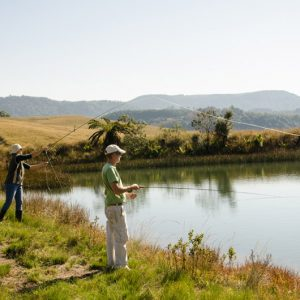
\includegraphics[scale = 0.8]{images/Casting.jpg}
  \caption{Fly Fishing on Rainbow dam.}
   \label{fig:FlyFishing}
\end{figure}



{\bf Dennis Dyer}

{\bf Fishing Committee Chairman}



% 
\chapter{History of Fishing at Mbona}

\section{The Vision}

Awesome Mbona! We, members of the Mbona Family, which extends over 50 years, 
have so much to be grateful and thankful for to a special few, headed up by Eric and Pat MacKenzie. 
What a profound vision they conceptualised, to build the paradise that we have all shared. 
Mbona has had a huge effect on our families and our children who have been able to free themselves 
of fear and many restrictions that have become a way of life in our country.
It is my pleasure and privilege to capture for you the history of trout and fishing as an additional recreation 
available to us on Mbona.

It all started one sunny day in late 1973 as Eric MacKenzie was walking close by the Crystal stream 
accompanied by a friend Edward Austin. Eric asked if there were any signs of fish in the area, 
Edward?s response was to catch a grasshopper and toss it into the stream. 
Almost instantaneously there was a swirl on the surface and the grasshopper was history, 
yes history in the making of trout fishing available to us. 

Such a simple beginning to a sport that has given so much joy to many.
Dams were mapped and designed with details of location demarcated. 
Drummond and Michael MacKenzie were tasked with naming each dam, 
they came up with the names that have become so familiar to us over the years, 
each having a special place in the hearts of enthusiastic anglers. 

They are:  Crystal, Rainbow, Laughter, Amber, Pateric, Emerald, Deep Pool, Evergreen and Holbeck. 
The list was sent to Pat and Eric, who were most impressed with the names. 
Pat was puzzled by the name which she pronounced Paterric for a short time until 
the penny dropped and she and Eric are forever remembered by the special name of this dam.

Today, it is so easy to name the dams, choose where we would like to fish and go 
and enjoy an experience that includes a magnificent environment, peace and quiet, birds, buck 
and occasional greetings to other shareholders as they walk or ride the many routes offered in our paradise. 
What we do not appreciate is the mammoth task that was undertaken to create these facilities. 
Crystal has a dam wall that is over 200meters long, how much earth works was needed is 
mind boggling and the cost in today?s standards would make it prohibitive to build. 
Each dam has been skilfully engineered and apart from Emerald, 
which has an irreparable leak, are functional all the year around.

\section{The Dams}

Some facts about Mbona dams:

\subsection*{Crystal,  21 hectares, 52 acres Completed in December 1972.}

Crystal is our largest dam. In the late 1976 a major rain storm occurred in and around Mbona. 
This resulted in a neighbouring dam above Evergreen, which had Bass in it, to overflow into Evergreen 
and to introduce Bass into its waters. It was decided to drain Evergreen which at that time was 
successful in getting rid of the Bass. Evergreen communicates with Crystal and the bass arrived 
and multiplied at a significant rate. The problem of the Bass in Crystal was the subject of much concern and debate. 
Draining of Crystal was not a consideration. After some time Bass were again seen in Evergreen. 
Today the consensus opinion within the Fishing Subcommittee is to rather create another facility for 
recreation so we have opened Crystal to a limited Bass fishing opportunity. 
Bass fishing is allowed with fixed spool reels and single hooked lures. Catch and keep is what is encouraged. 
This in fact has been a great boon to younger children, who now spend hours trying to catch bass and Bluegill 
which have also proliferated in Crystal. There have been no complaints received and in fact there have 
been a number of Bass caught between 3.5 and 5kg. Trout are caught in Crystal and one?s impression 
is that these numbers are on the increase which we believe is due to a more aggressive stocking program. 
Over the years there has been reference to concerns about reed encroachment in the southern end or inflow area between 
Laughter and Crystal. This is being discussed again, although it is a daunting task to dredge the area because 
silting up is the problem with the reeds flourishing in the enriched shallow water. 
There are discussions re creating a small wetland between Laughter and Crystal.

\subsection*{Evergreen,  10 acres. Completed 1975.}

Referred to above is the Bass problem in Evergreen and the floods in 1976. As noted Evergreen was drained 
and Bass exterminated, this was successfully done with people being asked to get rid of Bass by taking them 
home and trout were netted and transferred to Crystal.  Bass were back in Evergreen shortly after damage to 
the communication channel between Evergreen and Crystal had occurred. This was thought to be due to the 
fact that the Bass were able to swim up the damaged runway. Evergreen also had a problem with weed overgrowth 
and Grass Carp were introduced with good effect. There are no records relating to this, however, despite 
the fact that Grass Carp are supposed to concentrate their efforts on the periphery, the end result was positive. 
Of interest is that at one stage off Ernie?s walk, that circumvents Evergreen, a viewing platform was constructed 
5 meters above the water from which one could watch the fish swimming in the shallows. 
Grass Carp are now classed as exotic and it is virtually impossible to get hold of. Evergreen is a popular dam 
with floating tubes allowed, there are reports of excellent catches including some 3.5 kg bass. 
For some years it  was a catch and release dam, the fishing Committee at that time expressed their satisfaction 
with the outcome of this, however, other fishermen had had years of happy catching and preparing for the 
table and the decision to release has been recently lifted. If only our returns were more reliable, 
we could make a better than guessing as to the results.

\subsection*{Amber, 1 acre and Pateric, 2.5 acres, were both completed in 1973}

These two dams have regular reports of good catches. The recent blockage of the outlet from Pateric to Amber 
has been cleared and Amber has been overflowing for a good part of the year. Pateric has had leaks 
repaired on a number of occasions, however, every winter during the dry season, there is a significant drop in its level. 
A definite observation is that this dam is one of the most productive for catching trout and there is speculation that 
the nutrients available are due to enhanced growth of foliage during the low level periods.
Over the years Amber has produced a number of surprises of Rainbows over 2.5kg and a lone Brown of 2.2kg, 
this fish was returned to the water in good condition.

\subsection*{Rainbow: 3.2 acres, Laughter 4.2 acres, Deep Pool .75 acre and Holbeck 0.25 were all completed before the end of 1975.}

Rainbow has also had its catch and release restriction lifted, it is a very popular productive dam with a recent report of a 
2.5kg Brown caught and released.
Laughter has produced its share of excitement over the years. During the recent past there are no reports of Bass in this dam, 
although Bluegill are reported intermittently, however, 5 and 8 years ago there were Bass in Laughter. In both cases Laughter 
was drained and we have successfully rid  them of bass. There are a number of hypotheses mooted to explain this as there is 
no source of water that could be blamed as the source of the contamination. This included the possibility of fertile eggs attaching 
to the legs of water birds whilst visiting Crystal and then being transferred to Laughter. Our thoughts were more directed to 
suspect some human mischief. Since the last drainage, we have had no reports of Bass.
Each dam is unique and has a special attraction for a number of different fishermen. Both Holbeck and Deep Pool have been 
productive happy places for many of our shareholders. Holbeck is posing a problem with having silted up considerably. 
There are two camps, one wanting it to be left alone and the other hoping to dredge it and return it to its glory as a popular spot.

\section{The Hatchery}

The dams were eventually completed and we had the waters within which we could pursue our desire to enjoy fly fish for trout on Mbona.
The next step was to tackle the project of locating a source for trout, this led to the need to get in expert advice and guidance. 
This required a well thought out plan taking into consideration all the unique elements pertinent to Mbona. 
It was obvious that this was not just going to be an occurrence. It was going to be a long process that needed 
conscientious dedicated people to drive and maintain it. 
It needed financing and the blessing of the Joint Board of Directors who would support it financially and allow access to 
the permanent staff. This management team needed to be replicated as time went on and as the Board changed new 
people were needed to get involved. Throughout our history, we have had these people, 
many of them giving significant input of time and expertise. 

In December of 1973, the first joint board AGMeeting occurred. It was at this meeting that guidance from Terry Oatley 
was sought with respect to trout fishing at Mbona. Terry Oatley was a member of the Natal Parks Board and fortuitously 
was a shareholder at Mbona and this was one of his many contributions.
It was concluded that the location of Mbona, its elevation and its Climate would at best leave us with a situation that 
was marginal in our quest for creating a successful sporting and recreational facility 
for any of our interested shareholders. The initial decision was to stock our dams with 10inch fish. 
This was thought to be the most viable size to allow for optimal survival against weather conditions, predators such as otters, 
fish eagles and cormorants, the numbers of trout stocked in each dam was carefully worked out according to the volume of water 
in each facility, this is still being used as a guide today. Using Terry?s contacts, the Natal Parks Board documented a plan for Mbona. 
It was soon realised that the transport of the larger fish became a major operation which was both expensive and risky with 
quite a high mortality rate. The decision was made to buy 3000 6-7inch trout which had been calculated as a reasonable amount 
to stock our dams and support the fishing demands.

This meant that a facility needed to be built as rearing tanks for the fingerlings to grow them to the ideal stocking size of about 10inches. 
The basic plan was drawn up and this plan has evolved over the years to our present adequate and efficient system. 
There is a gravitational water supply from Lake Crystal to the ponds, which has had to be modified over the years. 
Some of the points are worth mentioning. We have developed this supply over the past 15 years so that it retains its original 
gravitational principle but so that it is adequate, we have created a dual system. This fulfils two essential functions, an adequate supply, 
which is at an appropriate depth to access the lowest water temperature, without being at too much risk of clogging up with 
debris and secondly is to have an adequate back up system. The fact is that the supply has been interrupted at least twice 
in the past with devastating results of wiping out the whole stock in the ponds. We have a rotational system in place where the inlets 
to these water supplies are checked regularly as part of our maintenance program. The quality of the water is enhanced by passing 
it through our aeration tower, which has also been modified at regular intervals. The new system also gives us the choice of 
increasing our water flow through the system, which is needed in the hotter months. We therefore have a quality, 
reliable and self-powered system which will be described in detail in the chapters that follow.

\section{Record Keeping}

One of the most significant developments in the last 10 years is the weighing and counting of the trout at the various stages of 
their lives in the hatchery. The handling has been perfected as are the methods of moving them from the ponds into the 
transporting vehicle, which is fitted with a tank that is well aerated and can accommodate 200 10 inch fish. 
This has allowed us to stock our own dams and deliver to customers, fish that are not compromised and mostly 
don?t even need any resuscitating. This is in contrast to previous efforts that always had a mortality rate. 
We have ensured a process that allows us to accurately size the fish for customers and also for record 
purposes of what is stocked and where.

 Record keeping of expenses has improved, accurate graphs on growth rate and feeding volumes is being 
 more accurately developed and maintained which will allow us to continue improving our production and 
 performance functionally and economically.
 
 The age old problem of monitoring once the fish have left the hatchery continues unabated. 
 From the beginning it was recognised the importance of outcomes of our efforts, fish returns, numbers of 
fishermen, the impact of catch and release initially and further down the line, 
the introduction of float-tubes and allowing them access now to Laughter as well as Crystal and Evergreen. 
Without this data, we will continue to make uneducated guesses rather than produce facts.

From the outset, fish returns have been notoriously poor. There have been a number of unsuccessful schemes, 
including sending a form with the monthly accounts to every shareholder. Apart from the new electronic accounts system 
introduced, this was not a success. Returns to the clubhouse, or the gate on leaving and now by email or on to the website 
are still poorly supported, we would appreciate any suggestions to add a catalyst to this process. 
The truth is, we are not able to assess the success of what we have done without appropriate data.


\section{Predators}
What has been shared is the development of the facility over the years to accommodate decisions made as part of the journey. 
To conclude this aspect, the original plan was well thought out and has not changed much, including the pitfalls to a perfect system. 
There have been a number of threats, apart from physical resource maintenance and development. 
The fish are vulnerable to predators even in the confines of the hatchery, shade cloth and nets are there to protect from birds, 
an electrified fence has been the most effective deterrent against otters, although the fence itself still needs attention to its strength. 
We still have a real, although mysterious reduction in numbers of fish from the raceway. It is our suspicion 
that there may be a human element to this phenomenon and the next step is to monitor by camera more frequently. 

\section{Acknowledgements}

As previously mentioned, the process was made possible by enthusiastic and interested individuals from conception 
to where we are today. Sharing with those involved, the success is always affected by the attitude of the joint board, 
the availability of funds, the management and the support of the trout and fishing committee. 
Over the years, we have been blessed by having these people to contribute to what we have today. 
A common thread commenting on the support and expertise of different managers every step of the way is 
evident and the present situation is better than any of us have experienced previously.

What a long exciting and productive journey this has been spanning fifty years. 
At the risk of not mentioning all the contributors to the epic, people who have been involved and made 
contributions are included as we summarise the progress over the years. Kindly accept apologies for any omissions. 

To Eric and Pat for their vision and the creation of the vast and superb infrastructure, including the dams, 
their beauty and their accessibility, the MacKenzie clan as well are the founders and to whom we will all be eternally enriched and grateful.

Over the years we need to acknowledge the invaluable support and contribution made by the respective Joint Board members. 
The services of managers, without exception, has been remarkable and appreciated by the trout committees. 
The original plan was researched by Ted Oatley, who used his contacts with the Natal Parks Board to produce a detailed assessment 
of the situation and then put together a plan of action. The basics of that plan are still being used today. 
We are in a process and this plan has been modified and developed to suit the needs of each successive committee.

The initial phase was to create the hatchery with the water supply from Crystal. The aerator was built, the three ponds created 
which were originally made of corrugated iron and the raceway. Garth Hatton was the first trout committee chairman. 
His services extended over the next 15 years, he has made a fantastic contribution over these years and was 
faced with many problems and also contributed to modifying the original plans to improve, not only the physical resources, 
but also the quality of the actual fishing. 

During his time he faced many challenges which included making the hatchery safer from predators, 
draining of Evergreen to get rid of the bass, increasing the capacity of the ponds as well as converting the ponds to brick and mortar, 
he rebuilt the aeration tower and produced a number of comprehensive reports which related to quality of the water in the dams, 
fishing rules and advice on stocking. He was well supported by the board and particularly the managers.

Chairmen that followed were among others, Richard Erasmus and Ken Cohen who was followed by 
first Nick and then Charles Shave who together served for more than 10 years up until 2005. 
All these men made every effort to maintain and improve conditions, each one has faced challenges including 
some disasters where large numbers of fish died. 
This was due to water supply failure, inclement weather conditions, otter invasions and even a few incidents of poaching. 
They were party to the decision to create catch and release restrictions in Rainbow and Evergreen, 
they retained the sourcing, purchasing and growing the trout, they were responsible for maintaining the hatchery 
and for seeing that the dams were properly stocked. They were continually devoted to improving the fishing as a quality recreation.

During the years, we have had expert advice and input from well known and respected trout fundies particularly 
Rob Karssing and Jake Alletson are acknowledged and thanked.

The present committee has been functional since 2005. They have faced all the problems of their predecessors 
including episodes of losses due to water blockages, maintenance of the hatchery and trying in vain to 
get better records of number of fishermen and their catches. An important decision was taken to buy trout eggs 
instead of buying fingerlings of 6 inches. This decision was taken in 2012 and it has changed our process 
considerably and has allowed us to increase our numbers substantially. The resources have been documented 
earlier in this article as well as the process of rearing the trout through the various phases of development. 
The venture has been successful.  We researched the process carefully and introduced scientific measures to 
measure temperature and oxygen content in the water accurately. 

We have improved the management of moving of trout and have got this down to a fine art. 
There has also been an improvement in all record keeping both monitoring growth and general running costs. 
The driving principle was to improve the fishing at Mbona primarily and secondly to sell fish of 30cms in size to neighbouring facilities. 
This has proved quite successful and we will continue to have frequent meetings, hoping to improve all of our ventures. 
We also took the decision to open Crystal to limited bass fishing as previously mentioned and to allow floating tubes on Laughter. 
The latter decision resulted in an exciting afternoon?s fishing producing over 20 nice sized fish. 
The committee is very active and meets regularly and would welcome new members, especially some younger enthusiasts.

There are a number of issues that we would really appreciate help with and suggestions one of  these is record keeping, despite the website facility, still leaves much to be desired. This is so important for us to know whether we are being successful or not and will guide in future plans. The Easter and Christmas fishing competitions are not as well supported as we would like. We are planning to supply trout to shareholders by an ordering system and would like to hear whether there is enough of a demand for them.

In conclusion, all previous contributors to this facility are to be saluted and thanked. 
The present committee has been active since 2005. It has been a great journey together of enthusiastic members 
doing research and development. This has been a shared experience. Each member has brought to the 
committee something special and all have been willing to attend meetings and especially to carry out tasks that they have undertaken to do. 

Jacko Jackson brought a wealth of scientific know how and expertise, 

Pierre Olivier has been a tower of strength with his practical experience and unrelenting service of maintenance, 
development and even deliveries is invaluable. 

Bernard McDonald always willing, contributed much knowledge and was always prepared to be hands on. 

Pete Barbour was our marketer and has established a nice clientele which has now been taken over by Ronnie Ritchie who is already producing results. 

It has been my privilege to work with this fine group of people. It must be said that Gareth Powell and Dave Forsyth have given us every support and assistance whenever we have asked and have made their contributions to what we have. 

We thank the boards over the years for their support and guidance. We believe that Mbona can be proud of our facility. 
We have as a first class entity that is functional and productive and that will continue to bring to shareholders a treasured resource. 
Any shareholders are welcome to come and see what we have in the hatchery and to be further informed of the process. 
We need some of our younger members to join us and take over.

We wish you great moments as you enjoy the unique and precious delights of Mbona and that you will at times be rewarded with a Rainbow trout of note.


{\bf Dennis Dyer}

{\bf Fishing Committee Chairman}











 

\pagestyle{headings}
\pagenumbering{arabic}

 

%\setcounter{chapter}{-1}

\chapter{Introducing Rainbow Trout}

\section{Trout Species}

There are 206 species in the family of {\it Salmonidae}. 
Salmonids (salmon, trout, char and whitefish) are found in practically all continents, 
partly because they are indigenous there and partly because they have been introduced.

Among trout, brook trout, brown trout, lake trout, sea trout and rainbow trout are the most 
widely known species.

\subsection{Brown Trout} 

Brown Trout are native to Europe and West Asia. An important market and sport fish, 
it has been introduced to many different countries all over the world, see figure  ~\ref{fig:BrownTrout}


\begin{figure}[H]
  \centering
   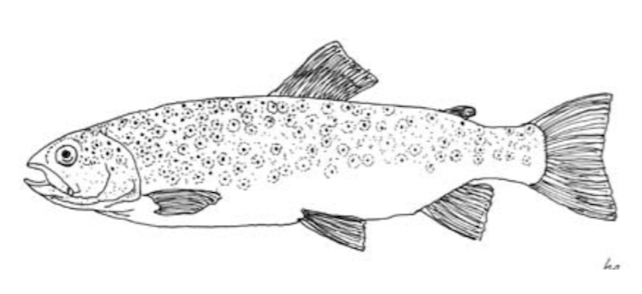
\includegraphics[scale = 0.5]{images/BrownTrout.png}
  \caption{Brown Trout.}
   \label{fig:BrownTrout}
\end{figure}

According to their habitat, taxonomists distinguish three forms of Brown Trout. 
They are the actual brown trout {\it Salmo trutta m. fario},  the
lake trout {\it Salmo trutta m. lacustris} and sea trout {\it Salmo trutta m. trutta},



\subsection{Brook Trout}

Brook Trout, together with Lake Trout {\it Salvelinus namaycush}, belongs to the {\it char} 
subgroup of salmonids, which distinguishes it from trout and salmon, see figure  ~\ref{fig:BrookTrout}

\begin{figure}[H]
  \centering
   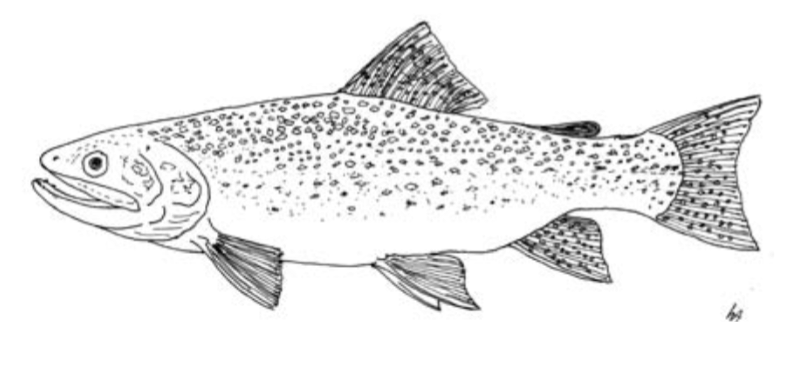
\includegraphics[scale = 0.5]{images/BrookTrout.png}
  \caption{Brook Trout.}
   \label{fig:BrookTrout}
\end{figure}

The Brook Trout is one of the most well-known sport fish and is native to the northeast of the United States of America and the east region of Canada. It has been introduced to many countries of South America, Oceania and Asia, and to practically all of the countries of Europe and the former Soviet Union.


\subsection{Rainbow Trout} 

Rainbow Trout, {\it Oncorhynchus mykiss}, is a highly commercial sport and market fish.
A normal adult rainbow trout weighs about 2-3 kg, while its maximum size, weight and age are 120 cm total length (TL), 25.4 kg and 11 years, respectively. Rainbow Trout live in the upper, cold water sections of rivers and seas, see figure  ~\ref{fig:RainbowTrout}

\begin{figure}[H]
  \centering
   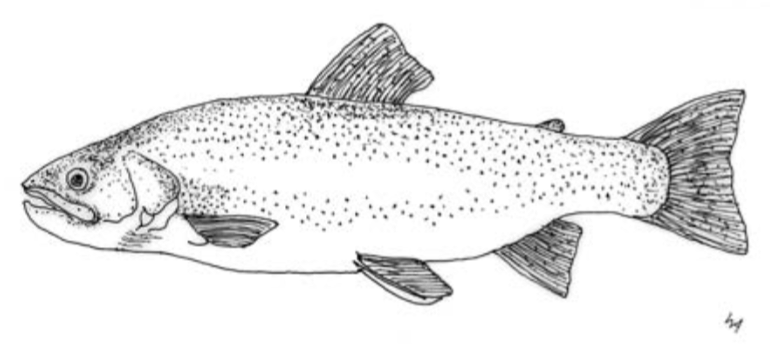
\includegraphics[scale = 0.5]{images/RainbowTrout.png}
  \caption{Rainbow Trout.}
   \label{fig:RainbowTrout}
\end{figure}

As in the case of other trout, the habitat and food of rainbow trout determine both their actual colour and shape.
The Rainbow Trout has many local strains, which have developed in the different river systems. Out of these, numerous improved commercial strains have been bred. The widely cultured commercial strains have been improved from those original rainbow trout populations that possessed advantageous qualities, such as hardiness, fast growth, resistance to diseases and reliable reproduction under farm conditions.


\section{Rainbow Trout in the Wild}

In the wild, there are rainbow trout populations that spawn in autumn and there are other populations that spawn in spring. From these populations, two different commercial strains have been bred. Their qualities are similar, only their spawning seasons differ from each other. This enables the production capacities of a rainbow trout farm to be increased.

\subsection{Habitat}
There are many habitat factors that basically influence the growth of rainbow trout. These include basic water qualities and the abundance of natural food.

A Rainbow trout is a typical cold water fish see the optimal temperature ranges in figure  ~\ref{fig:TempRanges}

\begin{figure}[H]
  \centering
   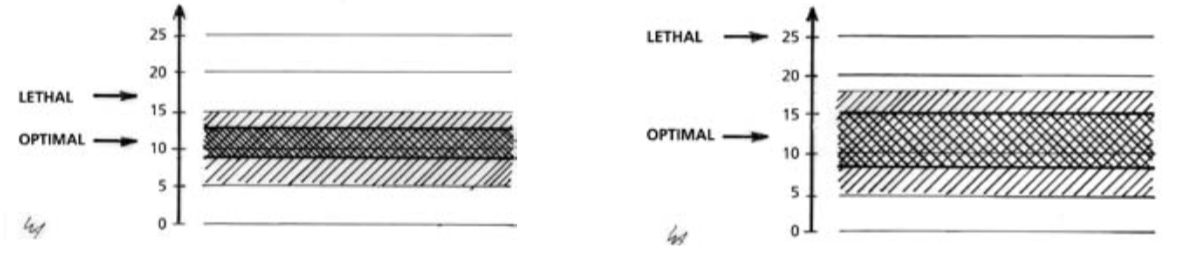
\includegraphics[scale = 0.7]{images/TempRanges.png}
  \caption{Optimal Temperature ranges for Rainbow Trout at different development stages: {\bf left:} during the incubation of eggs and sac fry, {\bf right:} during the growth. }
   \label{fig:TempRanges}
\end{figure}

Apart from temperature the other factors that influence growth are:

\begin{itemize}
\item[]Clear water: Keen eyesight is crucial for efficient feeding.
\item[]Dissolved oxygen: Water should sustain dissolved oxygen (DO) in high concentrations, in order to ensure smooth respiration. 
\item[]Clean water: Water should be free of harmful solid and gaseous waste materials produced during metabolism and respiration.
\end{itemize}


\subsection{Natural food} The natural food of rainbow trout depends on the age and size of fish, on the size of food item and on the habitat occupied. Rainbow trout are aggressive and greedy in feeding. They are opportunistic feeders that grab and eat almost anything. Figure ~\ref{fig:NaturalFood} summarises the most frequent natural food items of rainbow trout.


\begin{figure}[H]
  \centering
   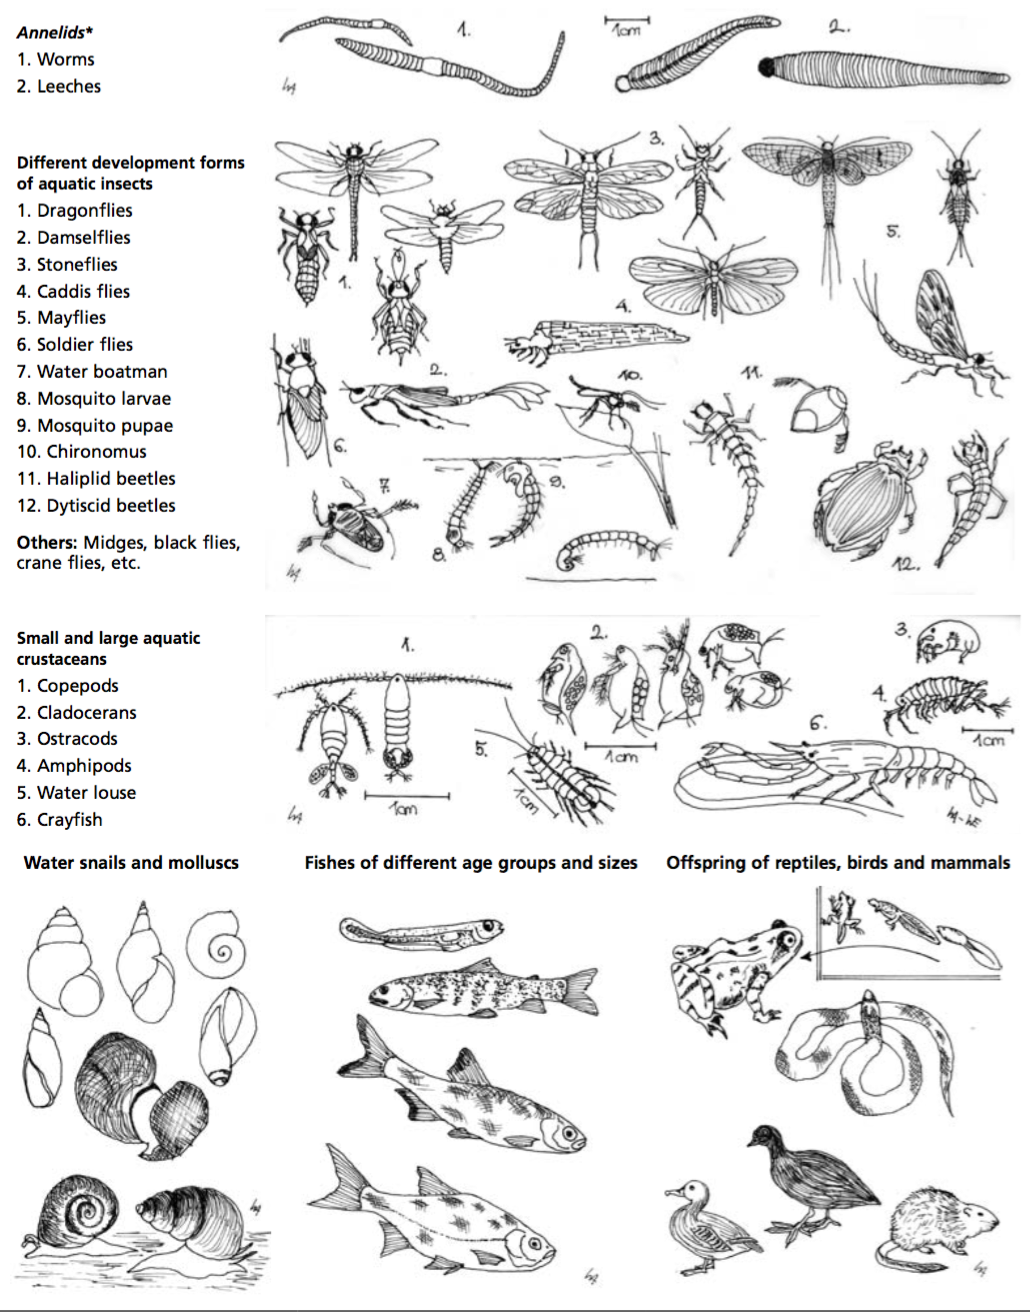
\includegraphics[scale = 0.5]{images/NaturalFood.png}
  \caption{Natural Food Sources for Rainbow Trout.}
   \label{fig:NaturalFood}
\end{figure}

Terrestrial insects are also consumed when they fall into the water. These insects are adult beetles {\it Coleoptera}, flies {\it Diptera}, ants {\it Formicidae} and larvae of moths and butterflies, {\it Lepidoptera}. 

\subsection{Life Cycle and Development Phases}

\begin{figure}[H]
  \centering
   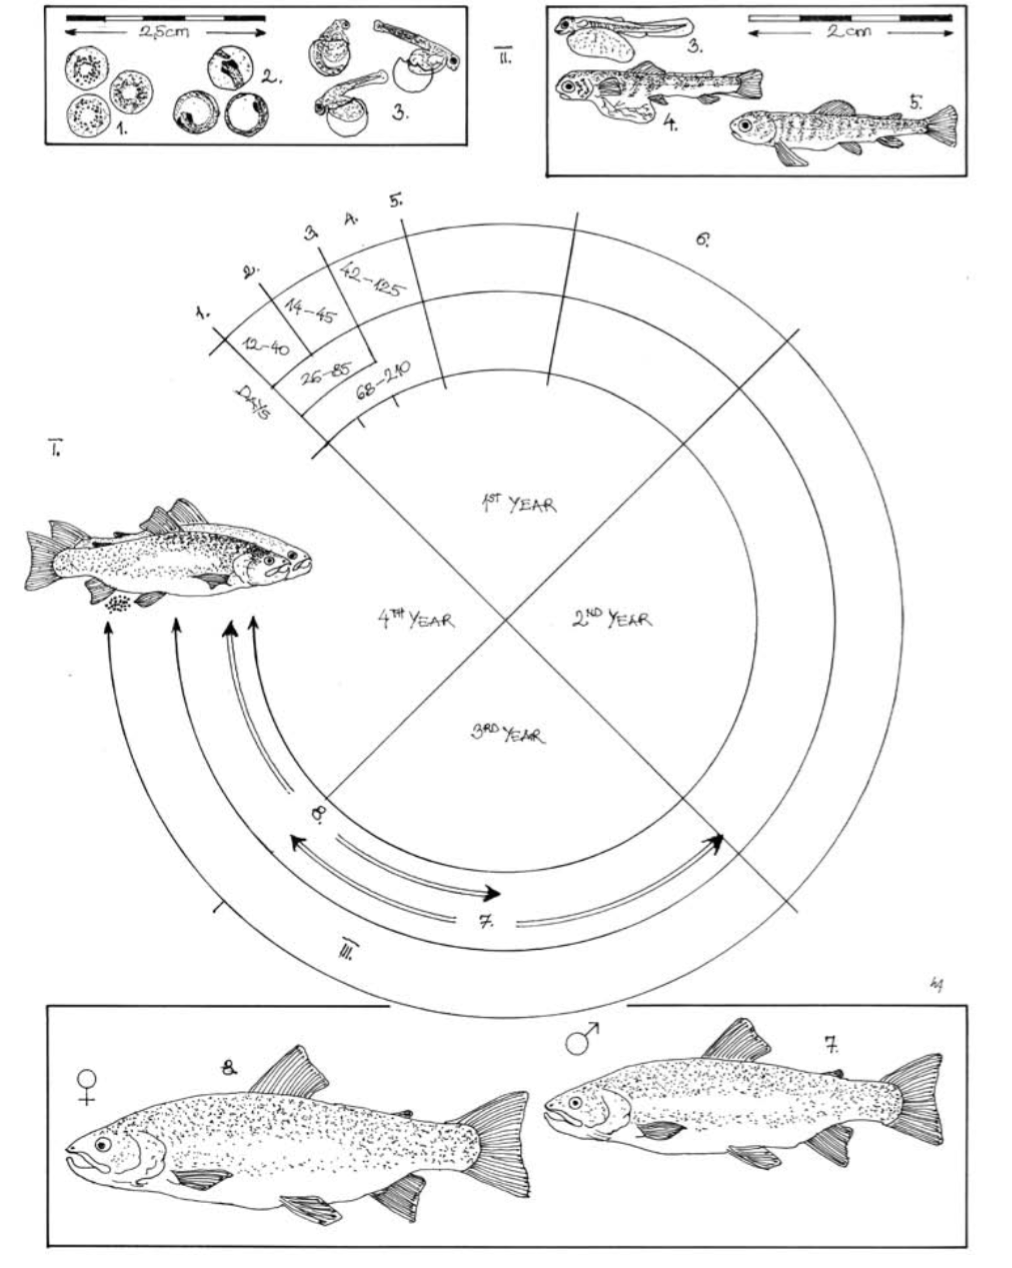
\includegraphics[scale = 0.6]{images/LifeCycle.png}
  \caption{Rainbow Trout Development Stages: 
  1. Fertilized eggs. 2. Eyed egg. 3. Hatched sac fry. 4. Swim-up fry. 5. Fry. 
6. One-summer fish. 7. Sexually mature male and 8. female ready to spawn}
   \label{fig:LifeCycle}
\end{figure}

Figure ~\ref{fig:LifeCycle} shows the life cycle and development stages for rainbow trout in the wild.
The actual start and duration of the different development phases depend on the water temperature, 
the genotype as well as the quantity and quality of available natural fish food.

\subsection{Body Parts}

Figure ~\ref{fig:BodyParts} and ~\ref{fig:LengthMeasurements} shows the body parts of a rainbow trout and the standard length measurements.



\begin{figure}[H]
  \centering
   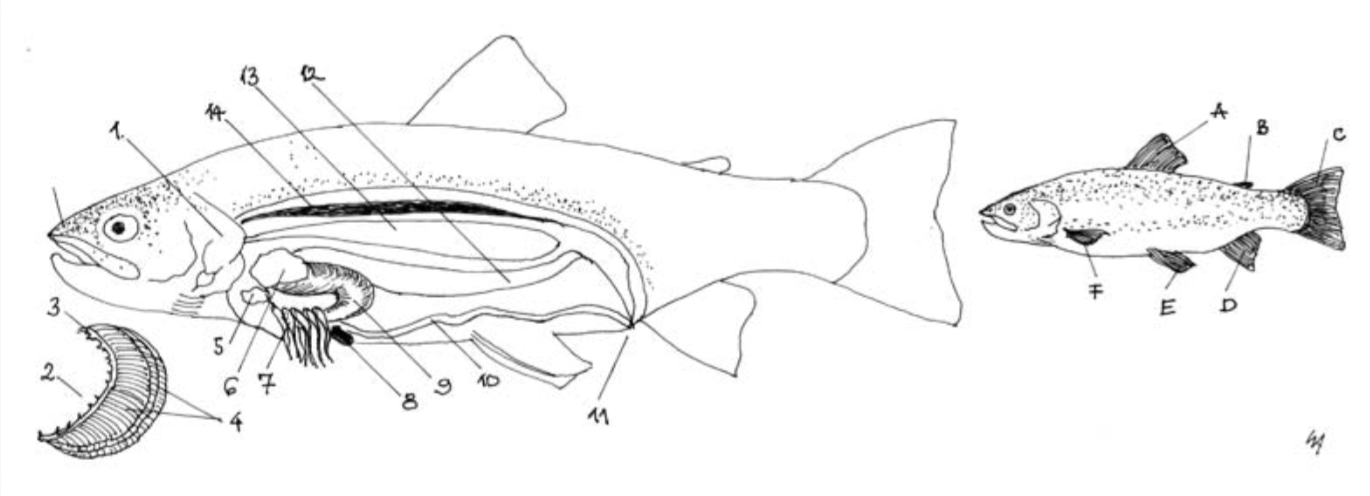
\includegraphics[scale = 0.5]{images/BodyParts.png}
    \caption{Rainbow Trout Body Parts: 
  1. Opercula (gill cover). 2. Gill raker. 3. Gill arch. 4. Gill filaments. 5. Heart. 6. Liver. 7. Pyloric caecae and pancreas. 8. Spleen. 9. Stomach. 10. Intestine. 11. Anus and urogenital papilla. 12. Gonad. 13. Swimming bladder. 14. Kidney. A. Dorsal fin. B. Adipose fin. C. Caudal fin. D. Anal fin. E. Pelvic fin. F. Pectoral fin.}
   \label{fig:BodyParts}
\end{figure}

\begin{figure}[H]
  \centering
   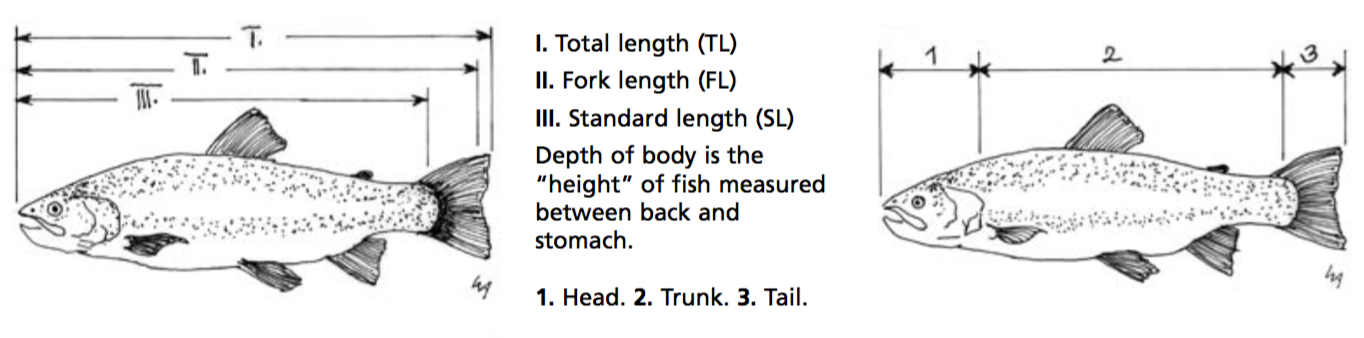
\includegraphics[scale = 0.6]{images/LengthMeasurements.png}
    \caption{Rainbow Trout Standard Length Measurements.}
   \label{fig:LengthMeasurements}
\end{figure}


\subsection{Length versus Weight}

Figure ~\ref{fig:LengthWeight} shows the correlation between its total length and weight.

\begin{figure}[H]
   \centering
   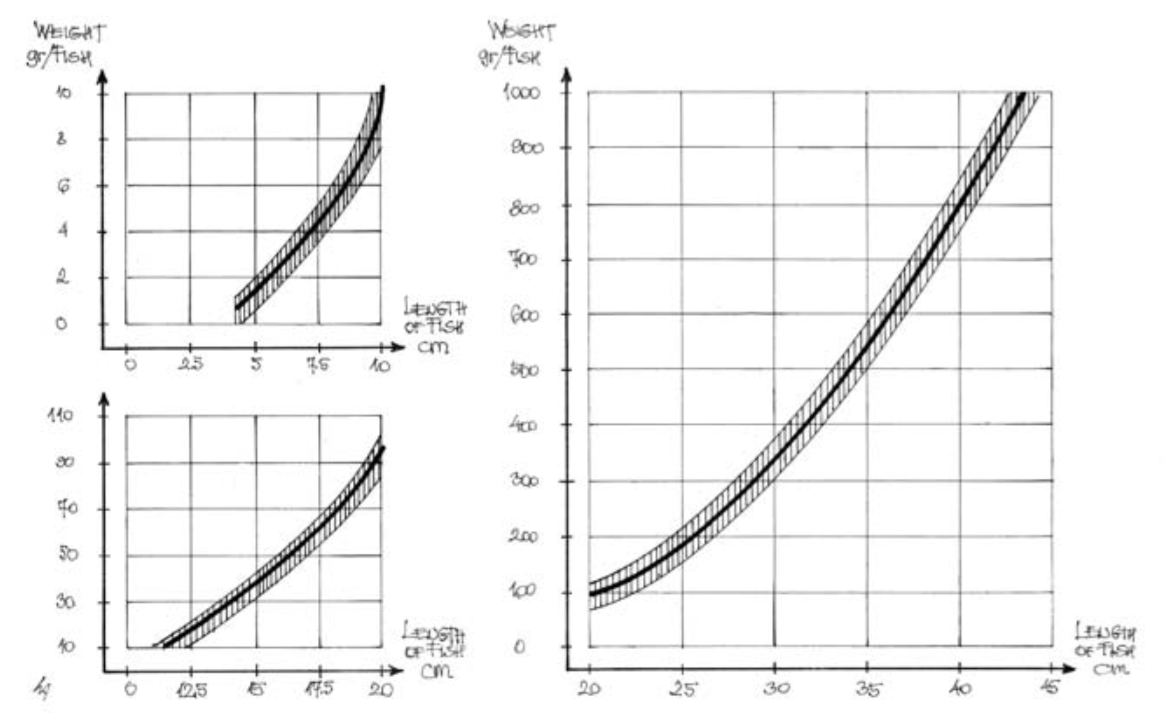
\includegraphics[scale = 0.6]{images/LengthWeight.png}
    \caption{Rainbow Trout Standard Length versus Weight Correllations.}
   \label{fig:LengthWeight}
\end{figure}

\subsection{Duration of development stages}

Water temperature is a major determining factor of fish production. 
This is because the body temperature of embryos, fry and developing fish equalise 
their temperature to that of the water they are in. 
Along with the body temperature, the intensity of the metabolism also changes.

The developing embryos and fry feed from the yolk sac and receive oxygen through the entire body surface. When the water temperature is higher, the embryos and fry develop more rapidly, while at lower water temperatures the speed of development reduces. Outside of a certain range of water temperature development stops.

\begin{figure}[H]
   \centering
   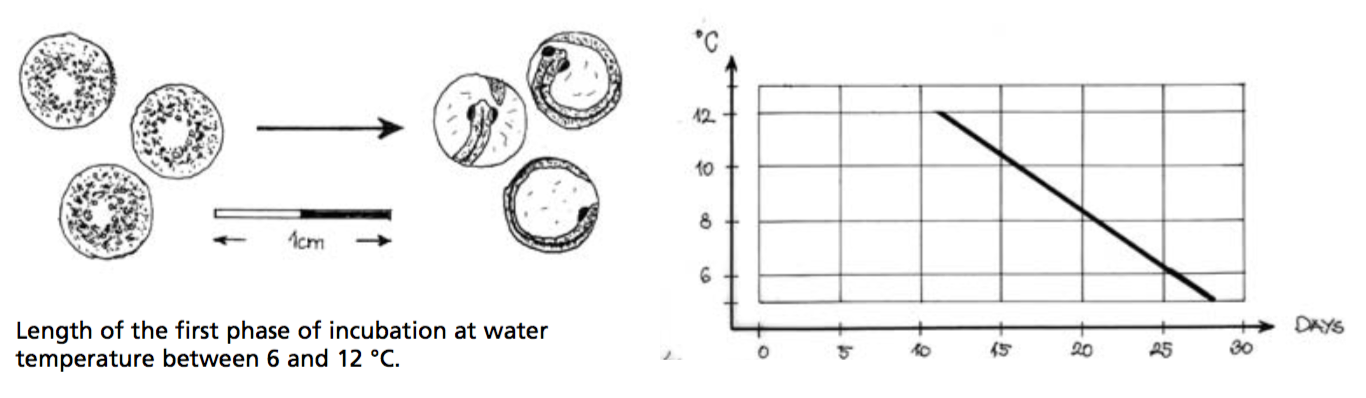
\includegraphics[scale = 0.6]{images/DurationIncubationFirstPhase.png}
    \caption{Duration of First Phase of Incubation.}
   \label{fig:DurationIncubationFirstPhase}
\end{figure}

\begin{figure}[H]
   \centering
   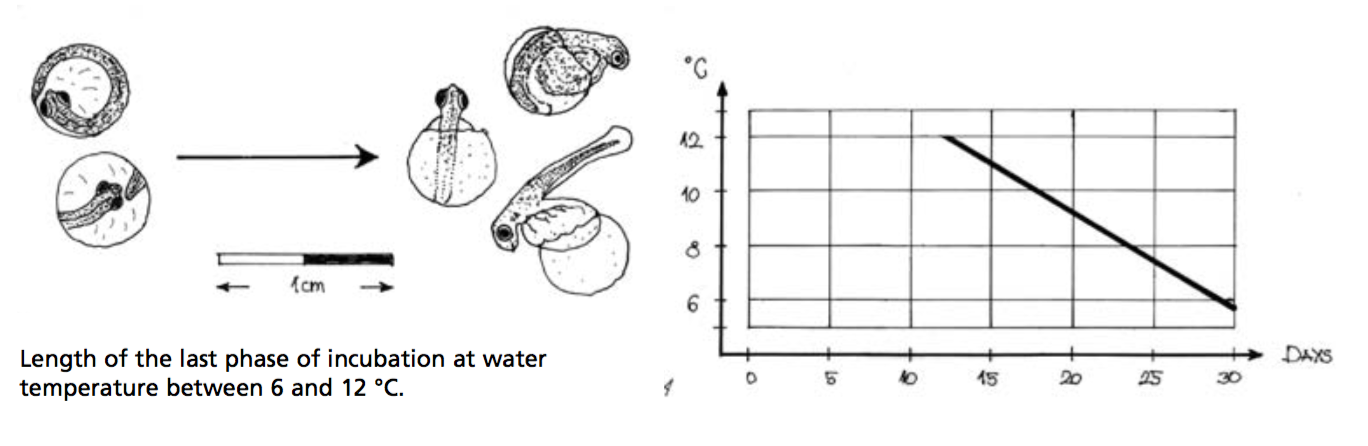
\includegraphics[scale = 0.6]{images/DurationIncubationLastPhase.png}
    \caption{Duration of Last Phase of Incubation.}
   \label{fig:DurationIncubationLastPhase}
\end{figure}

\begin{figure}[H]
   \centering
   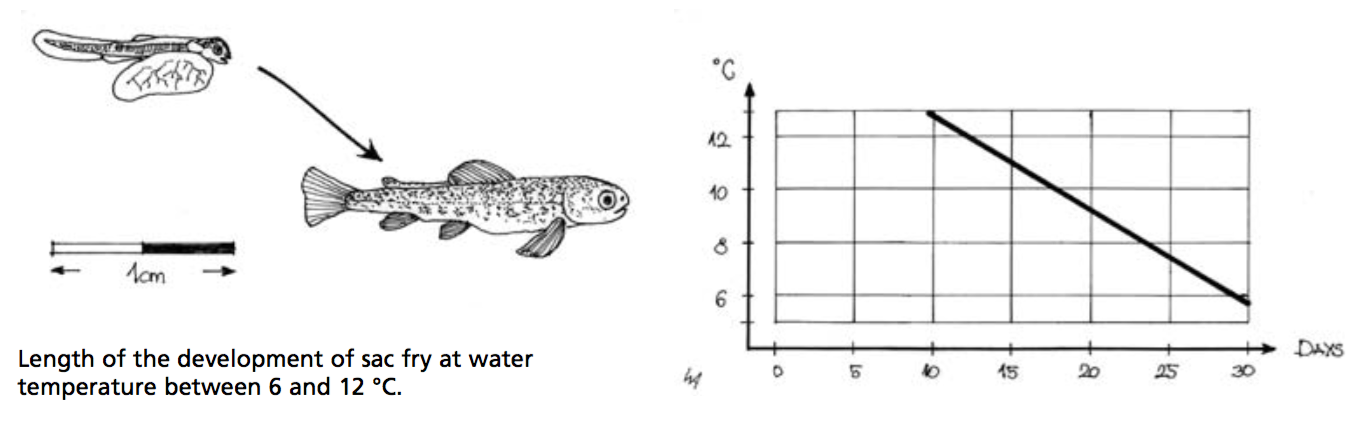
\includegraphics[scale = 0.6]{images/DurationSacFry.png}
    \caption{Duration of Sac Fry Development.}
   \label{fig:DurationSacFry}
\end{figure}

The total length of the development of embryo and fry from fertilisation to swim-up is about 37-83 days at water temperatures between  \SI{6}{\celsius} and  \SI{12}{\celsius}.

After starting external feeding, the actual length of the development of the different age groups depends not only on the temperature and oxygen content of water but also on the quality and quantity of consumed feed. Here, it has been assumed that trout is adequately fed with commercial feeds. 

Development of fry from swim-up fry takes 1.5-3 months, see figure ~\ref{fig:DurationSacFry}. Here. {\it fry} refers to a total length of 5 cm and to an average body weight of 2 g.

\begin{figure}[H]
   \centering
   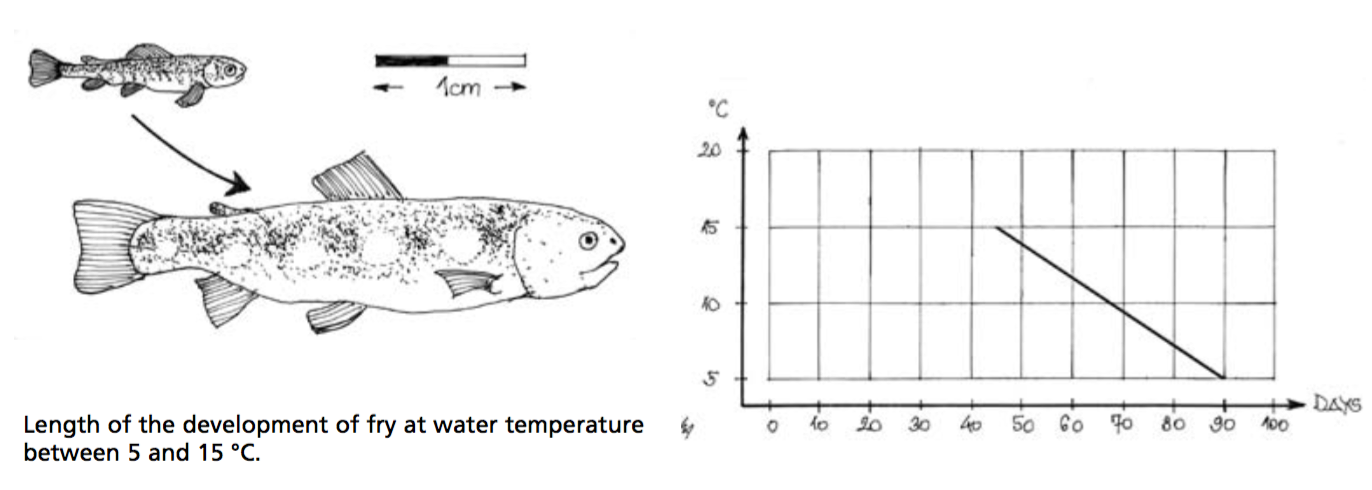
\includegraphics[scale = 0.6]{images/DurationFry.png}
    \caption{Duration of Fry Development.}
   \label{fig:DurationFry}
\end{figure}

Development of fingerlings from fry takes 3-4.5 months, see figure ~\ref{fig:DurationFry}. Here, {\it fingerling} refers to a total length of 12.5 cm and to an average body weight of 25 grams.

\begin{figure}[H]
   \centering
   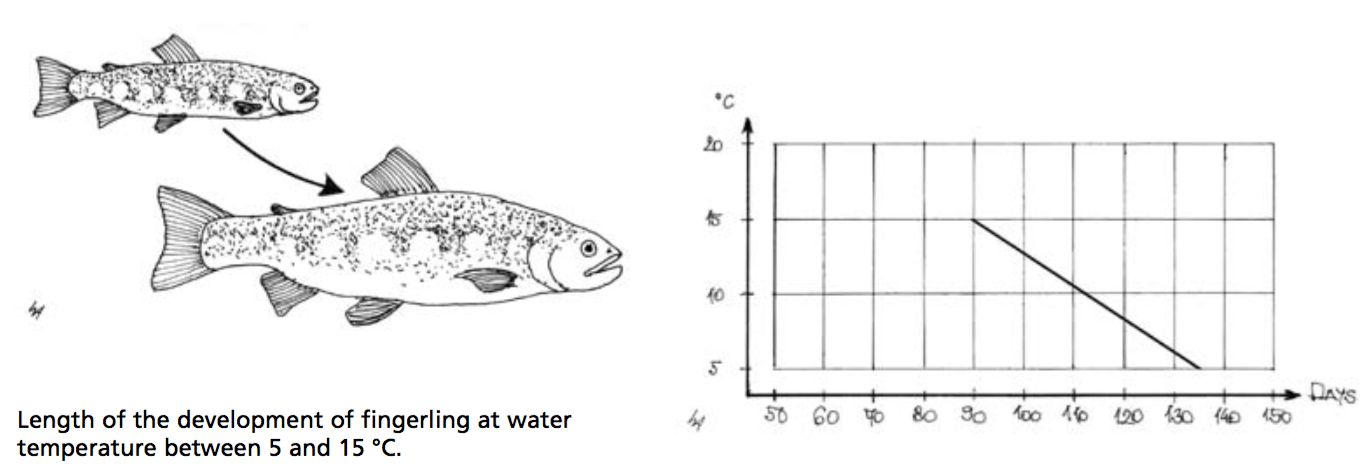
\includegraphics[scale = 0.6]{images/DurationFingerlings.png}
    \caption{Duration of Fingerling Development.}
   \label{fig:DurationFingerlings}
\end{figure}

Development of table fish from fingerling takes 4-6.5 months,  see figure ~\ref{fig:DurationFingerlings} . Here, {\it table fish} refers to the desired minimum body weight of 250 g.

\begin{figure}[H]
   \centering
   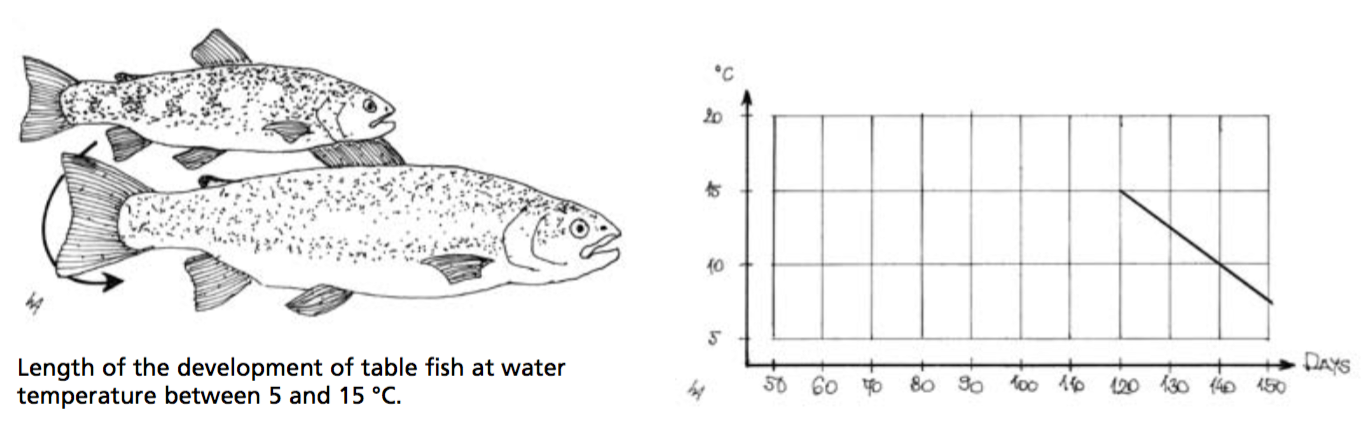
\includegraphics[scale = 0.6]{images/DurationTableFish.png}
    \caption{Duration of Table Fish Development.}
   \label{fig:DurationTableFish}
\end{figure}

Growth of large table fish from 250 g to 500 g takes a further 2.5-4.5 months (75-135 days) when the water temperature is between  \SI{5}{\celsius} and  \SI{15}{\celsius}.



\section{Production Conditions}

In this section we outline the optimal or near to optimal conditions that should be ensured during production of the different age stages of Rainbow Trout. 

\subsection{Water pH} 

Rainbow Trout tolerates unfavourable pH conditions differently during the various development phases of the fish. The optimal and acceptable ranges of pH of rearing water also differ. For developing embryos and fry, the range of optimal pH is narrow, and varies between 6.5 and 8, but the range of acceptable pH is also narrow. For older fish, both the optimal and acceptable ranges of pH are wider, as demonstrated in figure ~\ref{fig:OptimalPH}.

\begin{figure}[H]
  \centering
   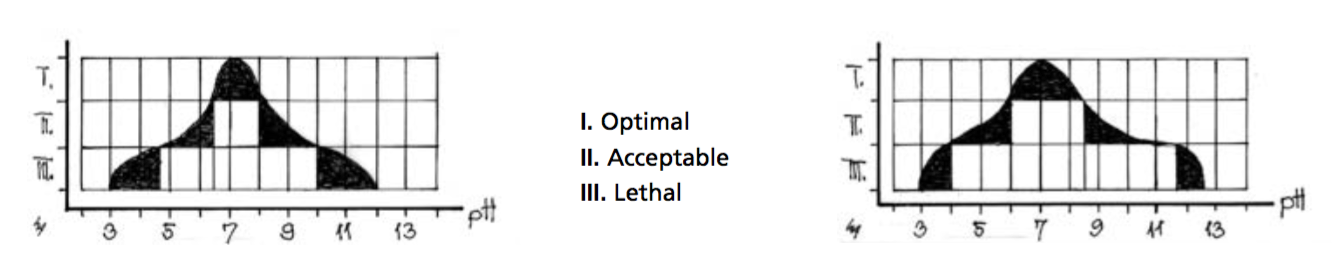
\includegraphics[scale = 0.5]{images/OptimalPH.png}
  \caption{Optimal pH ranges for embryos and swim-up fry on the left and growing fish on the right.}
   \label{fig:OptimalPH}
\end{figure}


\subsection{Water Temperature} 

The optimal, acceptable and lethal ranges of water temperature also vary according to the development stages of the fish, as demonstrated in figure \ref{fig:OptimalTemp}.

\begin{figure}[H]
  \centering
   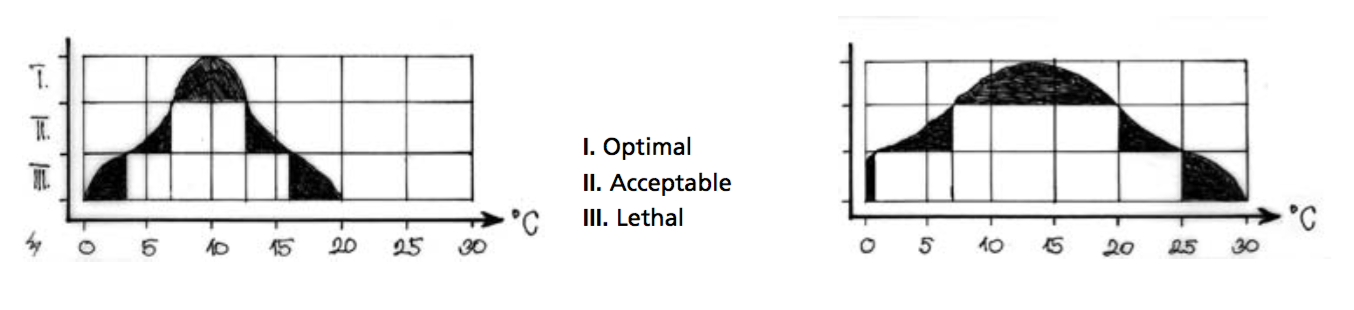
\includegraphics[scale = 0.5]{images/OptimalTemp.png}
  \caption{Optimal temperature ranges for embryos and swim-up fry on the left and growing fish on the right.}
   \label{fig:OptimalTemp}
\end{figure}


There is a range of water temperature, about \SI{7}{\celsius} to \SI{18}{\celsius}, where the appetite of feeding rainbow trout is optimal, see figure \ref{fig:OptimalAppetite}. Outside of this range, at lower and higher water temperature, fish lose appetite. Finally, at too low or too high water temperature, fish stop feeding.

Feed intake of rainbow trout intensifies as the water temperature increases. However, this behaviour continues only up to about \SI{18}{\celsius}.  Above this temperature, the appetite of and feed intake by the fish sharply decreases and stops.

\begin{figure}[H]
  \centering
   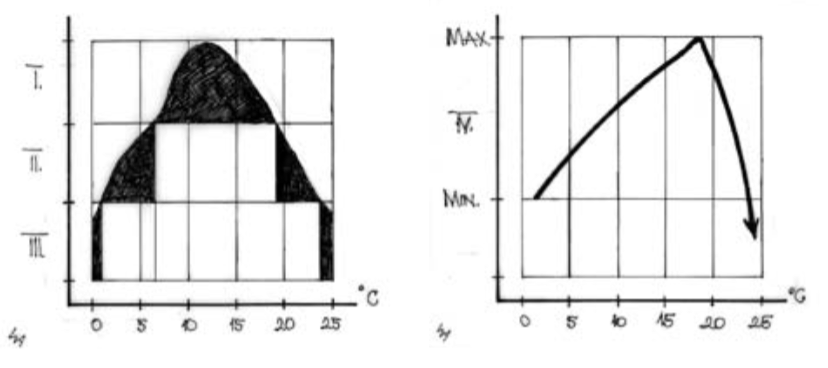
\includegraphics[scale = 0.5]{images/OptimalAppetite.png}
  \caption{ I. Optimal range of appetite. II. Losing appetite. III. Feeding stops. IV. Intensity of feeding..}
   \label{fig:OptimalAppetite}
\end{figure}

It is important to be aware that there is an inverse correlation between the intensity of feeding and the utilisation of consumed feed. Thus, at about \SI{18}{\celsius}, rainbow trout are willing to feed very intensively, but the digestion of consumed feed will be less complete at this temperature. The water temperature where the different trout species make the best growth out of the consumed feed varies from \SI{13}{\celsius} to \SI{15}{ \celsius}. 

\subsection{Water Oxygen Content}

Oxygen dissolved in water ensures the respiration of the different aquatic plants and animals. 
Most frequently, the DO content of water is expressed in milligrams of oxygen per litre of water (mg/litre).
The maximum oxygen content of water depends on the water temperature. 
This is because water can dissolve only a certain quantity of oxygen, which is determined by the partial pressure of oxygen in the atmosphere.
Figure ~\ref{fig:OxygenTemp} shows the inverse correlation between temperature and DO content of water. 
At a higher temperature of water, the DO content is lower. 
At maximum oxygen content, water is 100 percent saturated with oxygen and the oxygen in excess soon leaves to the atmosphere.

\begin{figure}[H]
  \centering
   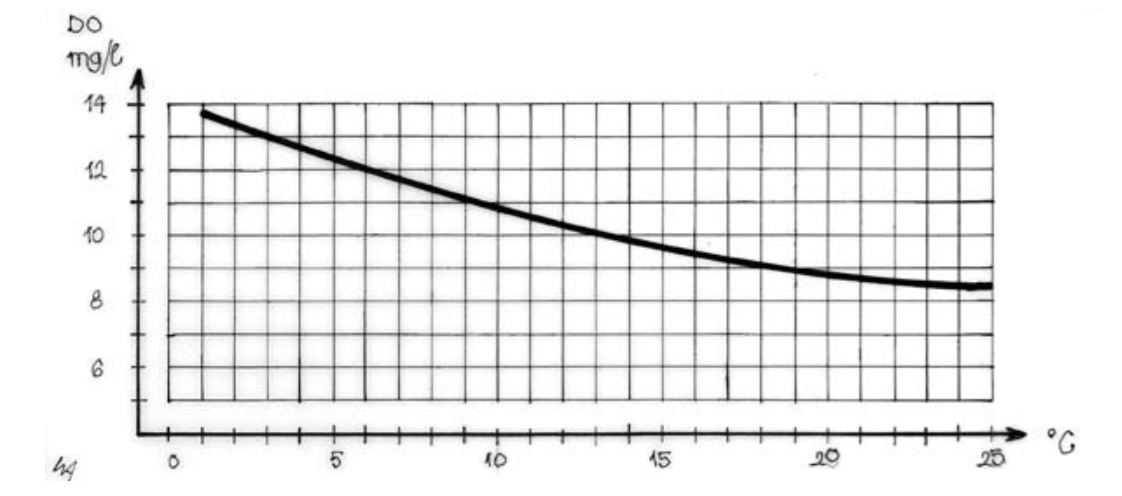
\includegraphics[scale = 0.5]{images/OxygenTemp.png}
  \caption{ Correlation between temperature and maximum oxygen saturation.}
   \label{fig:OxygenTemp}
\end{figure}


The optimal and acceptable concentrations of oxygen in water vary according to the actual development stage of the fish. The optimum is when the oxygen content of rearing water is near to saturation (100 percent). The acceptable range of oxygen content of rearing water is lower. It ranges between 5 and 6 mg/litre during incubation of eggs and the first development stages of fry. For older age groups, the acceptable low oxygen content of water may be about 4.5 mg/litre.

It is important to know that the oxygen consumption of fish increases considerably during and after feeding. During these periods the demand for oxygen will temporarily increase.

\subsection{Water Supply}

In order to ensure the replacement of used water in the rearing devices, a continuous supply of fresh, clean and oxygen-rich water is essential. The necessary quantities of water supplied depend on the age and actual quantity of the developing fish.

The quantity of eggs, fry and growing fish per unit area of rearing device is determined by the oxygen content of supplied water. In colder water, the metabolism and, hence, respiration slows, while in warmer water they intensify. Accordingly, the actual quantity of water needed for the same number of developing embryos, fry and fish will be different. At low water temperature, the quantity of water supplied may be less but at higher water temperature it should be more. See figure ~\ref{fig:WaterSupply} 

\begin{figure}[H]
  \centering
   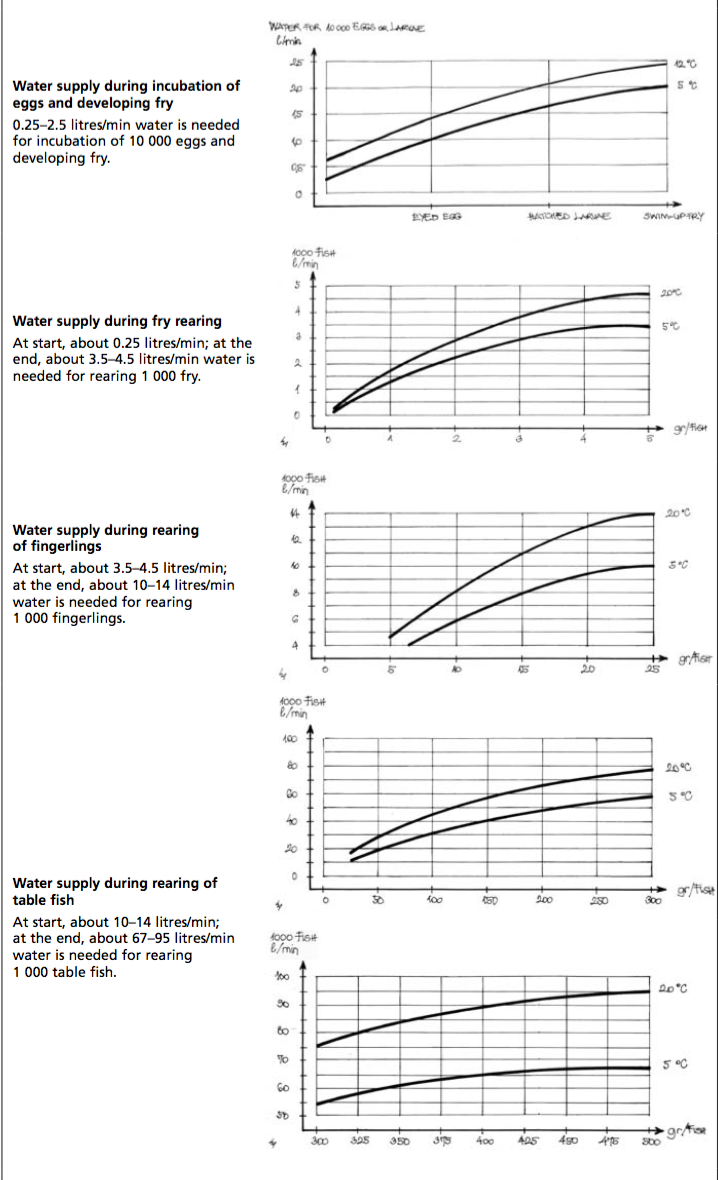
\includegraphics[width=8cm]{images/WaterSupply.png}
  \caption{ Water supply in tanks required according to development stage of fish. }
   \label{fig:WaterSupply}
\end{figure}


Water supply is expressed by the flow rate, which is the quantity of water needed for 10 000 specimens of eggs or 1 000 specimens of fry or fish. It is expressed either in litres per second (litre/s) or litres per minute (litres/min). 

Frequency of water exchange is another way to specify the quantity of supplied water. It is expressed by the exchange rate of water per hour or day.

The water supply in concrete or lined tanks can be more intensive than in earth ponds, hence the density of fish can also be higher in these devices.

\subsection{Aeration Principles}

In the practice of pond fish farming oxygen deficiency has been regarded as dangerous mainly because 
of mass losses of fish. But recent investigations have shown that decreased oxygen saturation can 
have serious effects on the economy of a fish farm as well.

Keeping the dissolved oxygen content of the pond water nearly at the saturation level makes it possible 
not only to avoid mass losses of fish but ensures better conversion rates and higher yields in intensive culture.

Most trout farms use flow-through systems, whereby grow-out tanks are continuously refreshed 
with large quantities of new water, usually gravity-fed from nearby streams or rivers. 
Whether rectangular raceways or self-cleaning circular tanks are employed, 
the essentials remain the same; rapid removal of wastes and 
continuous replenishment of the system with highly oxygenated water.


\chapter{Mbona Hatchery}

\section{Infrastructure.}

At the Mbona Hatchery we make use of Baths, Tanks and Ponds for the production of fry, fingerlings and table fish, see ~\ref{fig:HatcheriesLayout} for the layout of the Mbona Hatcheries operation.

\begin{figure}[H]
  \centering
   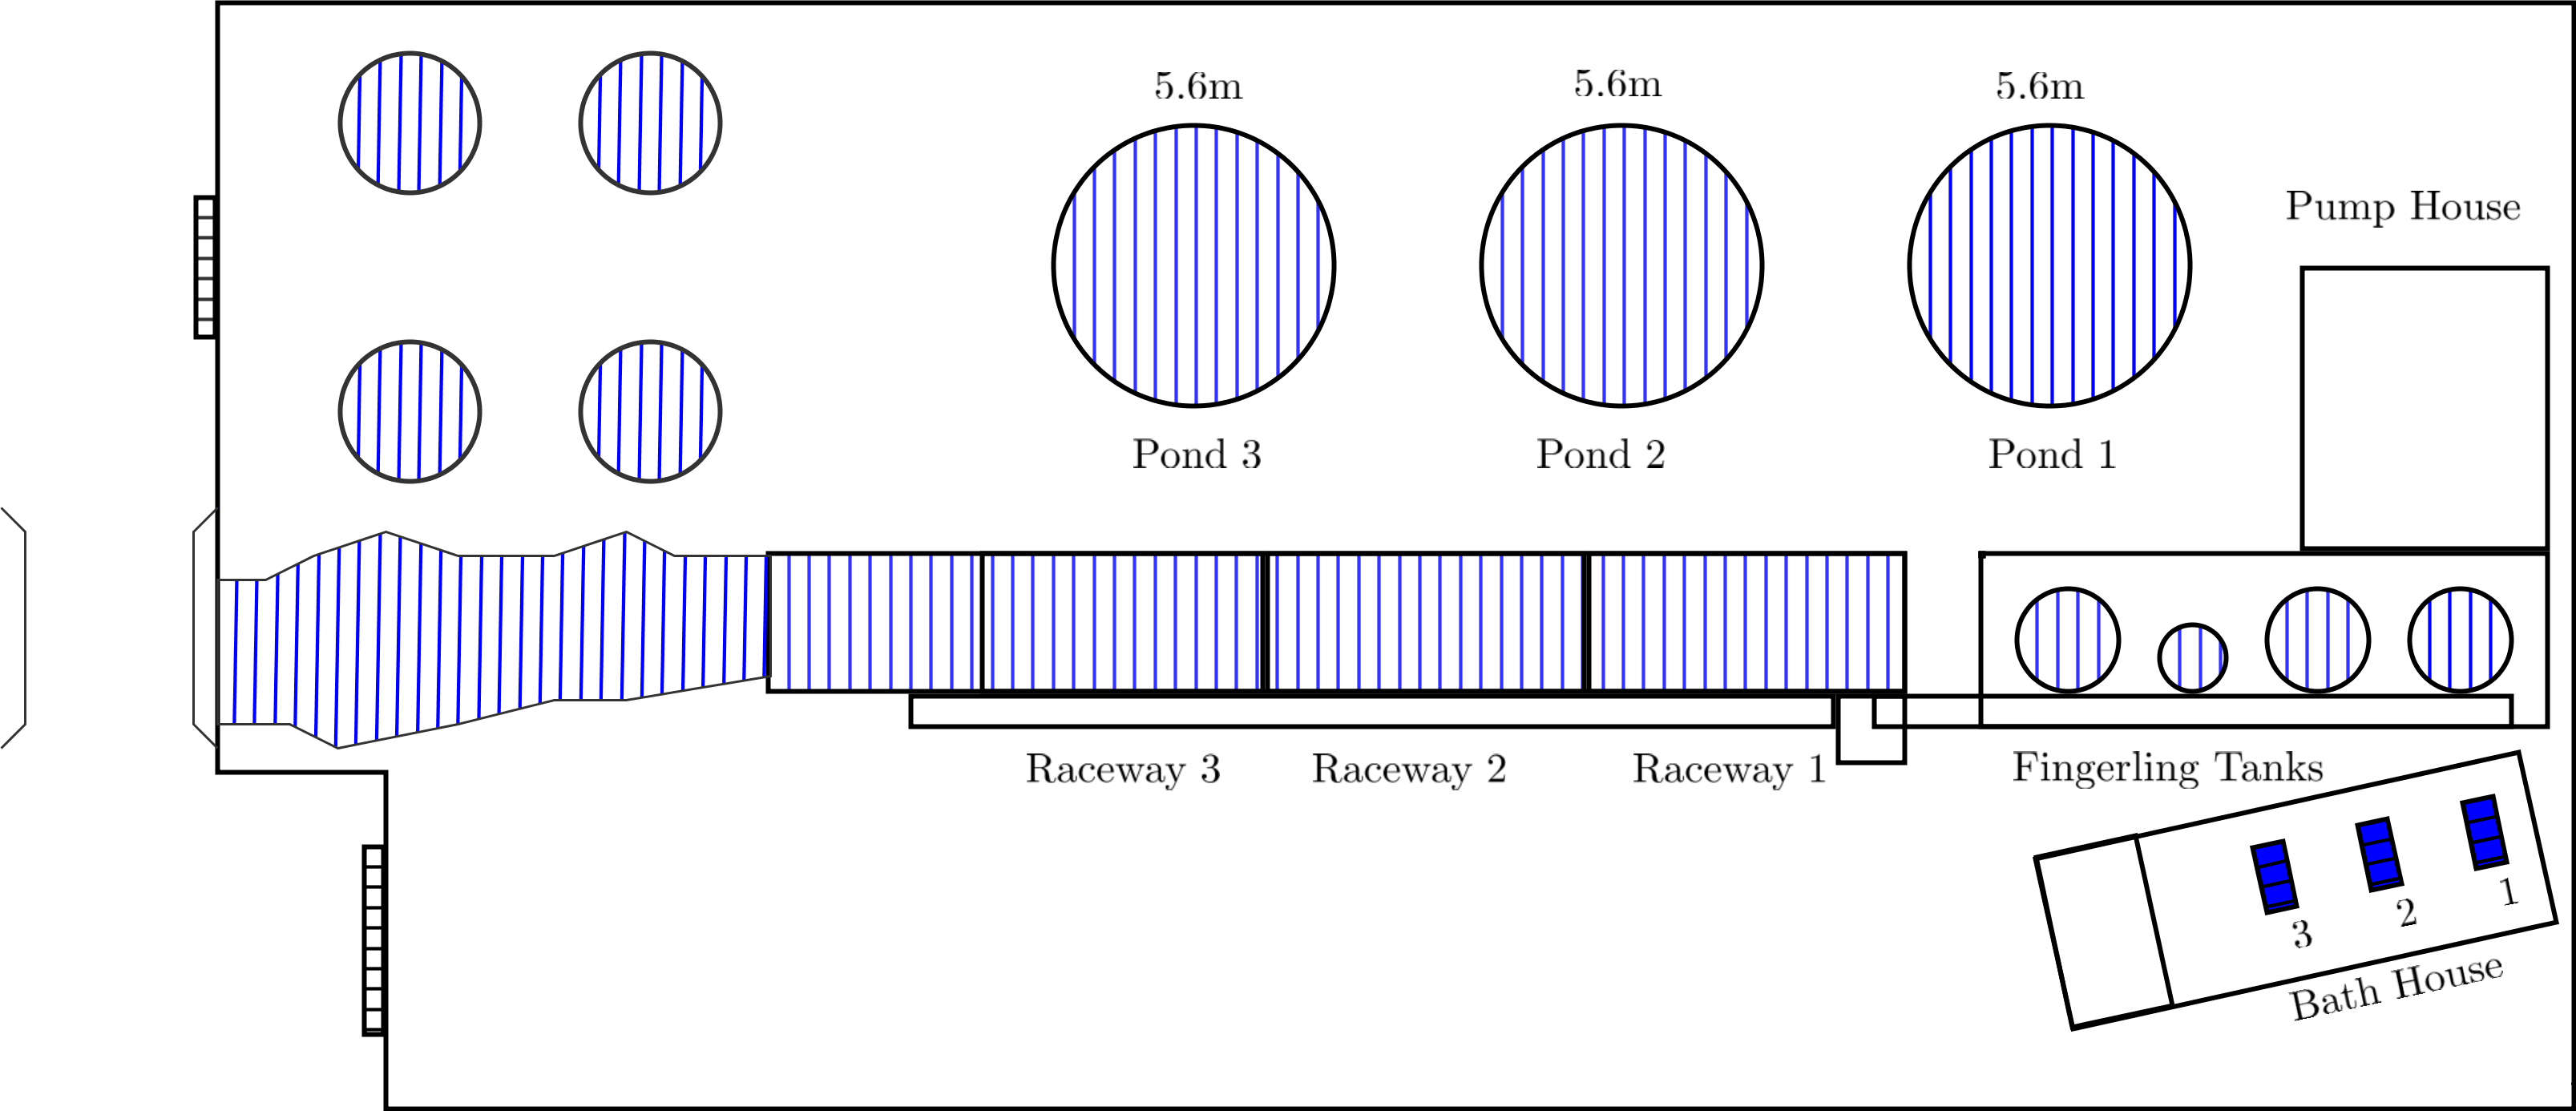
\includegraphics[scale = 0.15,angle=0,origin=c]{images/HatcheriesLayout.png}
  \caption{Mbona Hatcheries Layout.}
   \label{fig:HatcheriesLayout}
\end{figure}

\subsection{Hatching Baths} 

At the Mbona Hatchery we use a California hatching tray which is a screened, flat-bottomed tray that fits horizontally inside the rearing bath and is arranged so that water is forced through the eggs from below.

The tray is a container for incubation of eggs and sac fry. The bottom of the tray is a sieve material, on which the eggs and sac fry rest. They are placed in a Hatching Bath and they receive freshwater through the sieve from under the tray, as illustrated in figure~\ref{fig:HatcheryBaths}. 

\begin{figure}[H]
  \centering
   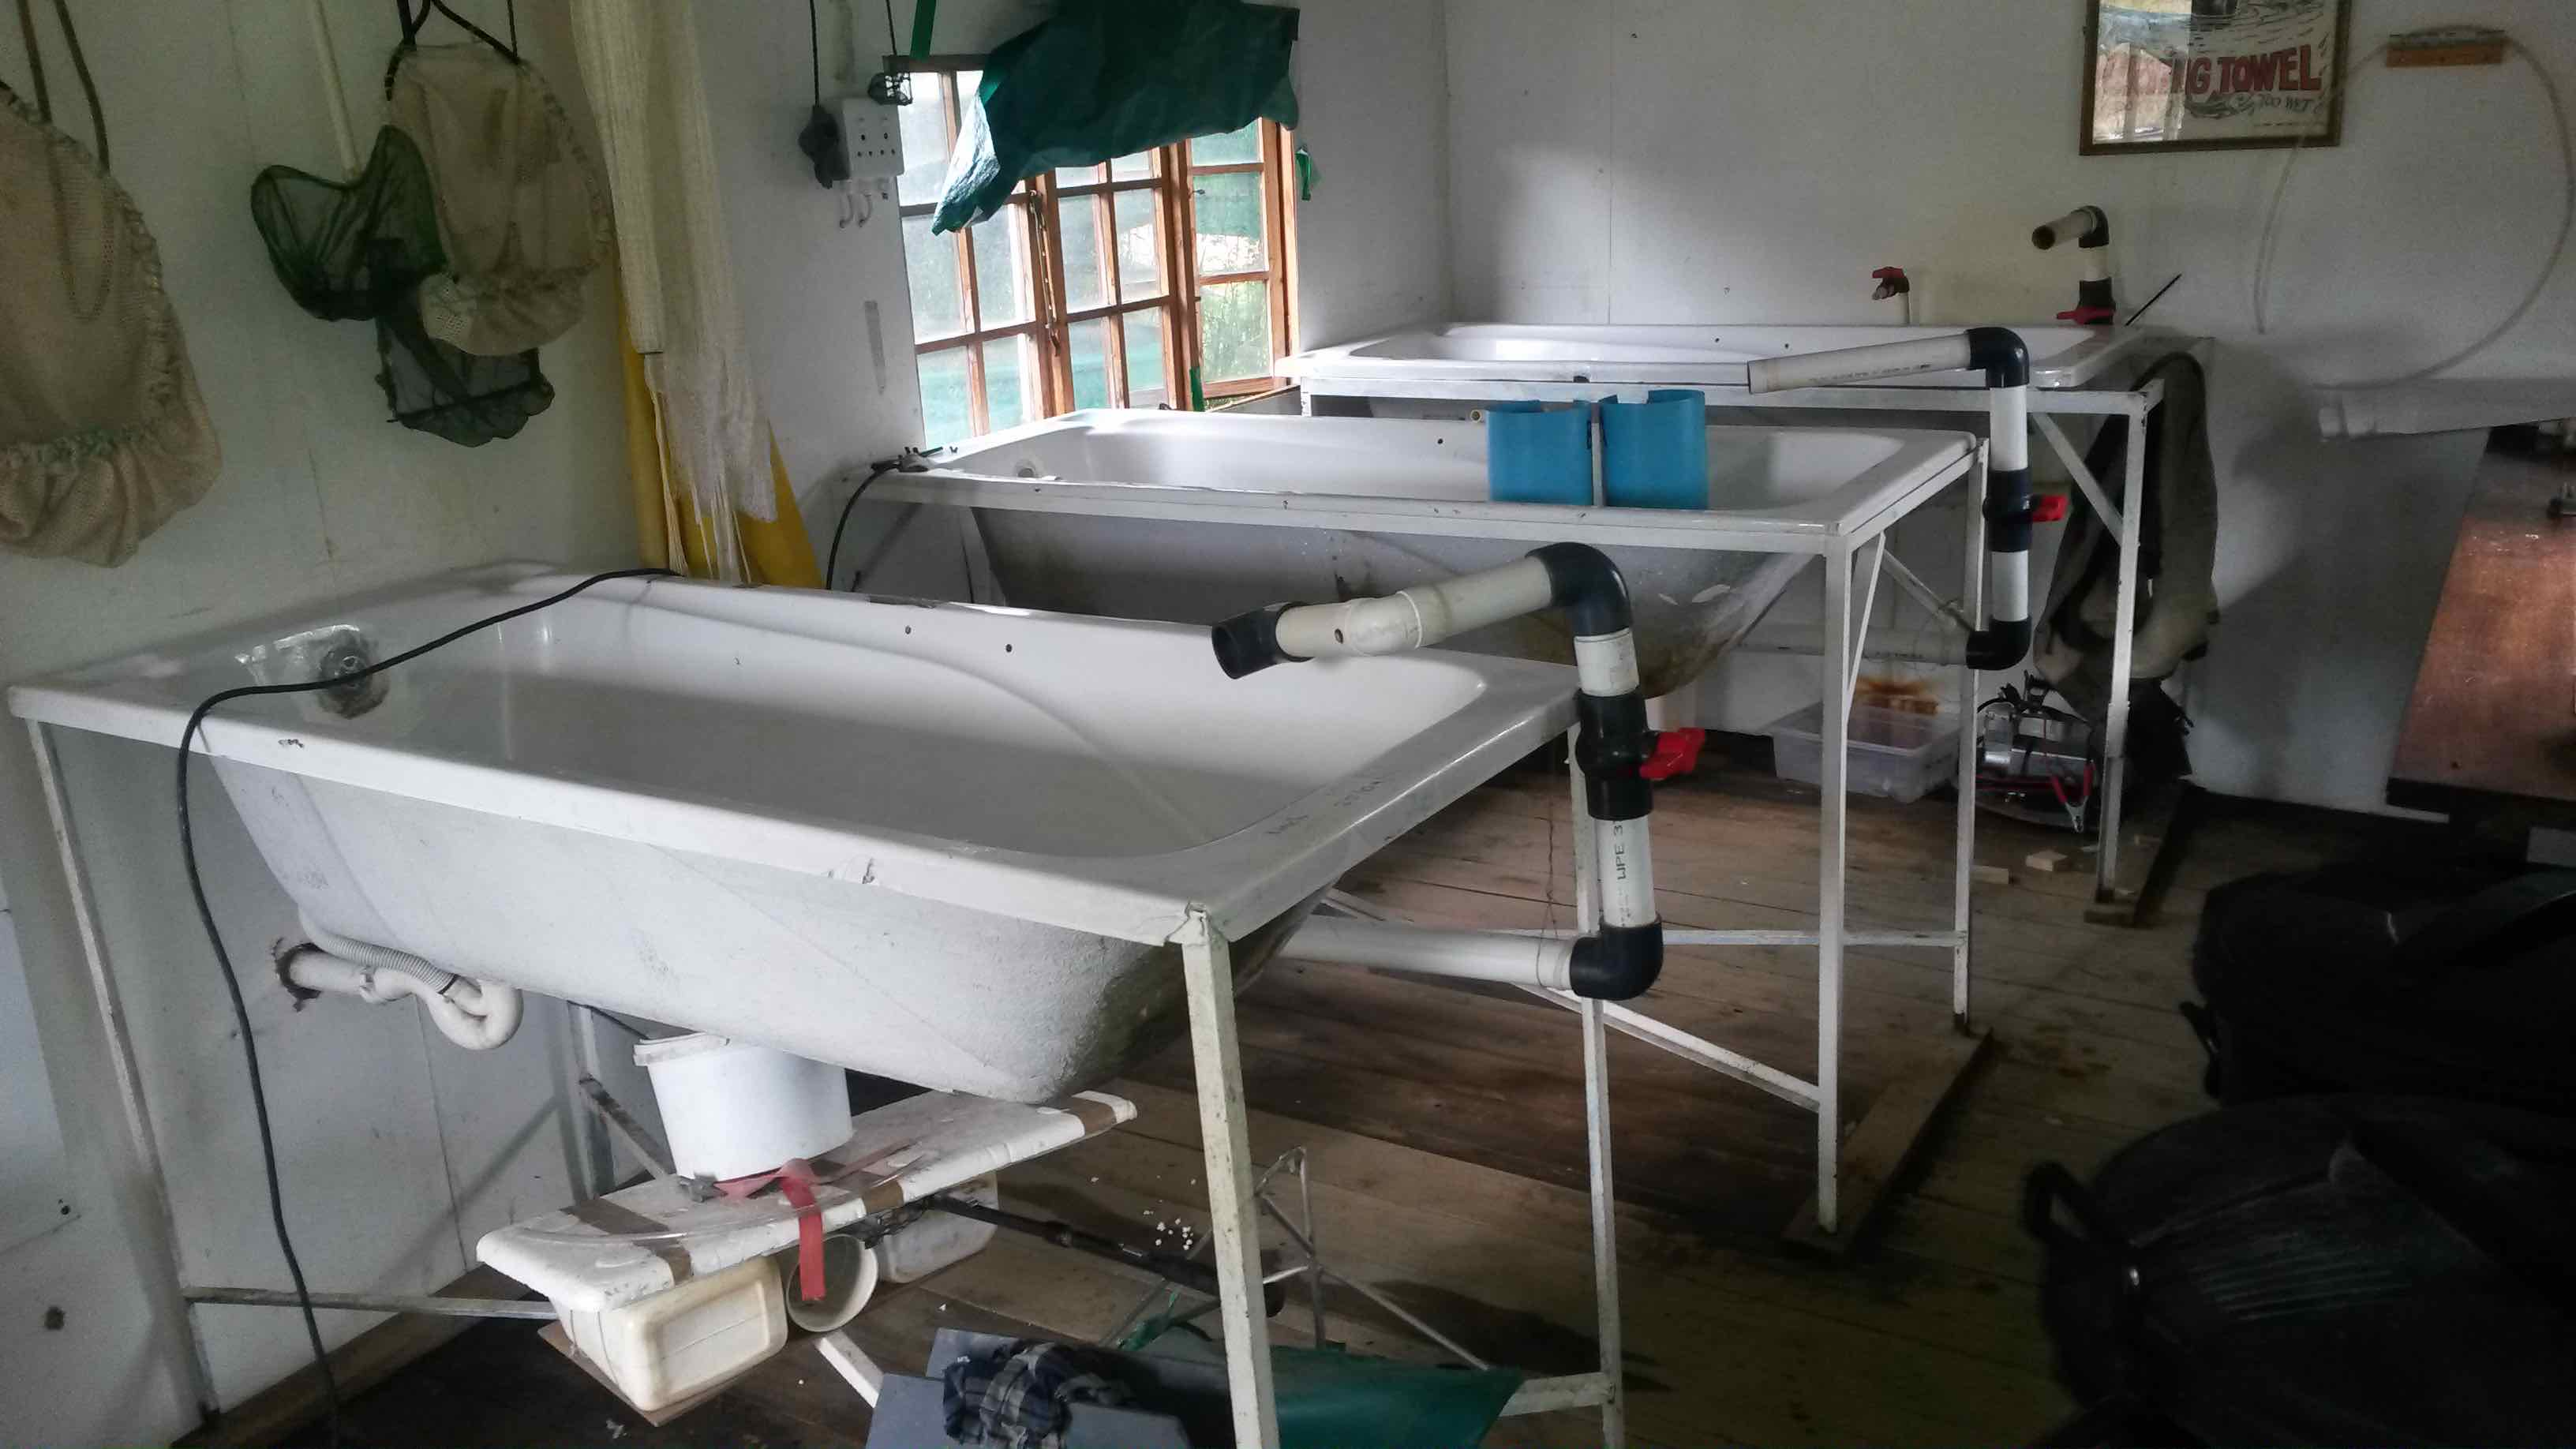
\includegraphics[scale = 0.1]{images/HatcheryBaths.jpg}
  \caption{Mbona incubator baths have one California type tray (size: 0.5 m � 0.4 m = 0.2 m2). When hatching trays are removed, the bath is used for rearing the fry.}
   \label{fig:HatcheryBaths}
\end{figure}


Although the material, shape and size of hatching trays may vary, the quantities of eggs and sac fry that can be incubated on them are similar. A hatching tray about 0.2 meter squared is needed for the incubation and hatching of 10 000 rainbow trout eggs. Later, the required space increases, because 10 000 swim-up fry need 5 times more space (about 1 meter squared) with about 0.5 m depth. The required quantity of water in these devices should be ensured and adjusted as presented in the graphs of the previous chapter.

\subsection{Fry Tanks}

\begin{figure}[H]
  \centering
   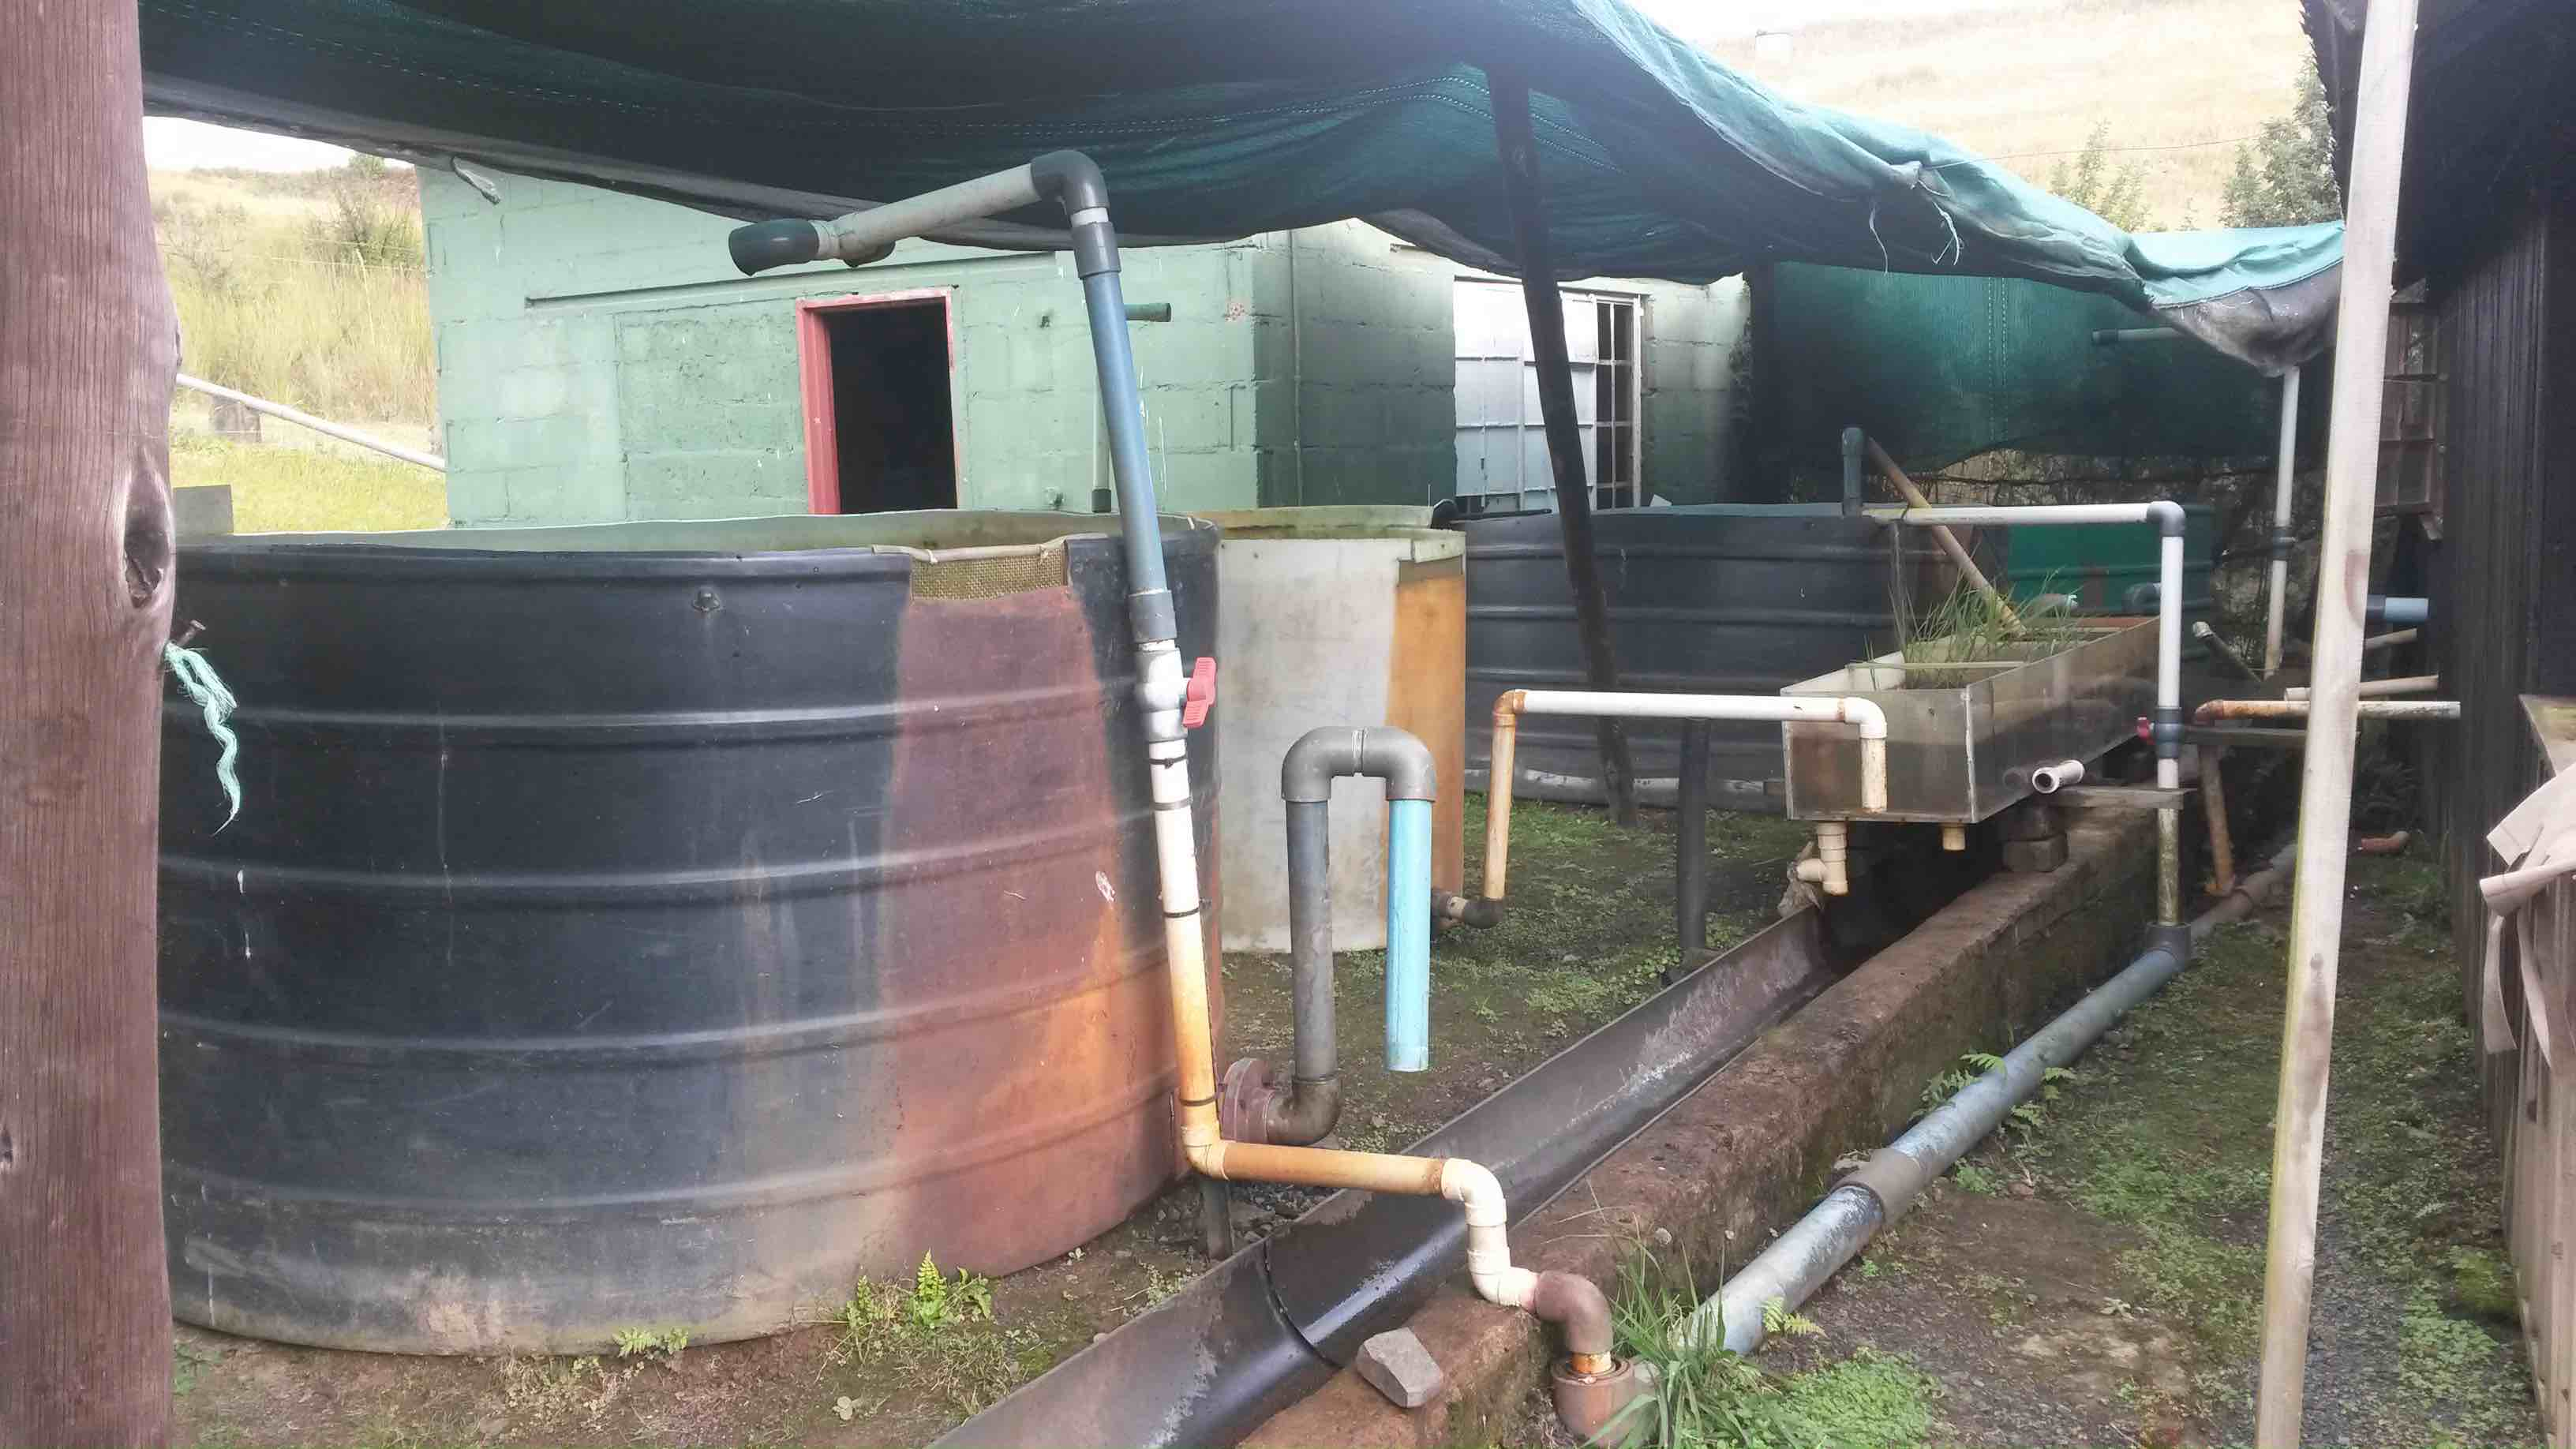
\includegraphics[scale = 0.1]{images/HatcheryTanks.jpg}
  \caption{Mbona fry tanks are plastic jojo type tanks used for rearing the fry till they are old enough to move to the tanks. The flow rate through the tank is controlled by an inlet valve and the depth of water in the tank is determined by the height of the overflow outlet pipe. }
   \label{fig:HatcheryTanks}
\end{figure}



\subsection{Growing Ponds}

\begin{figure}[H]
  \centering
   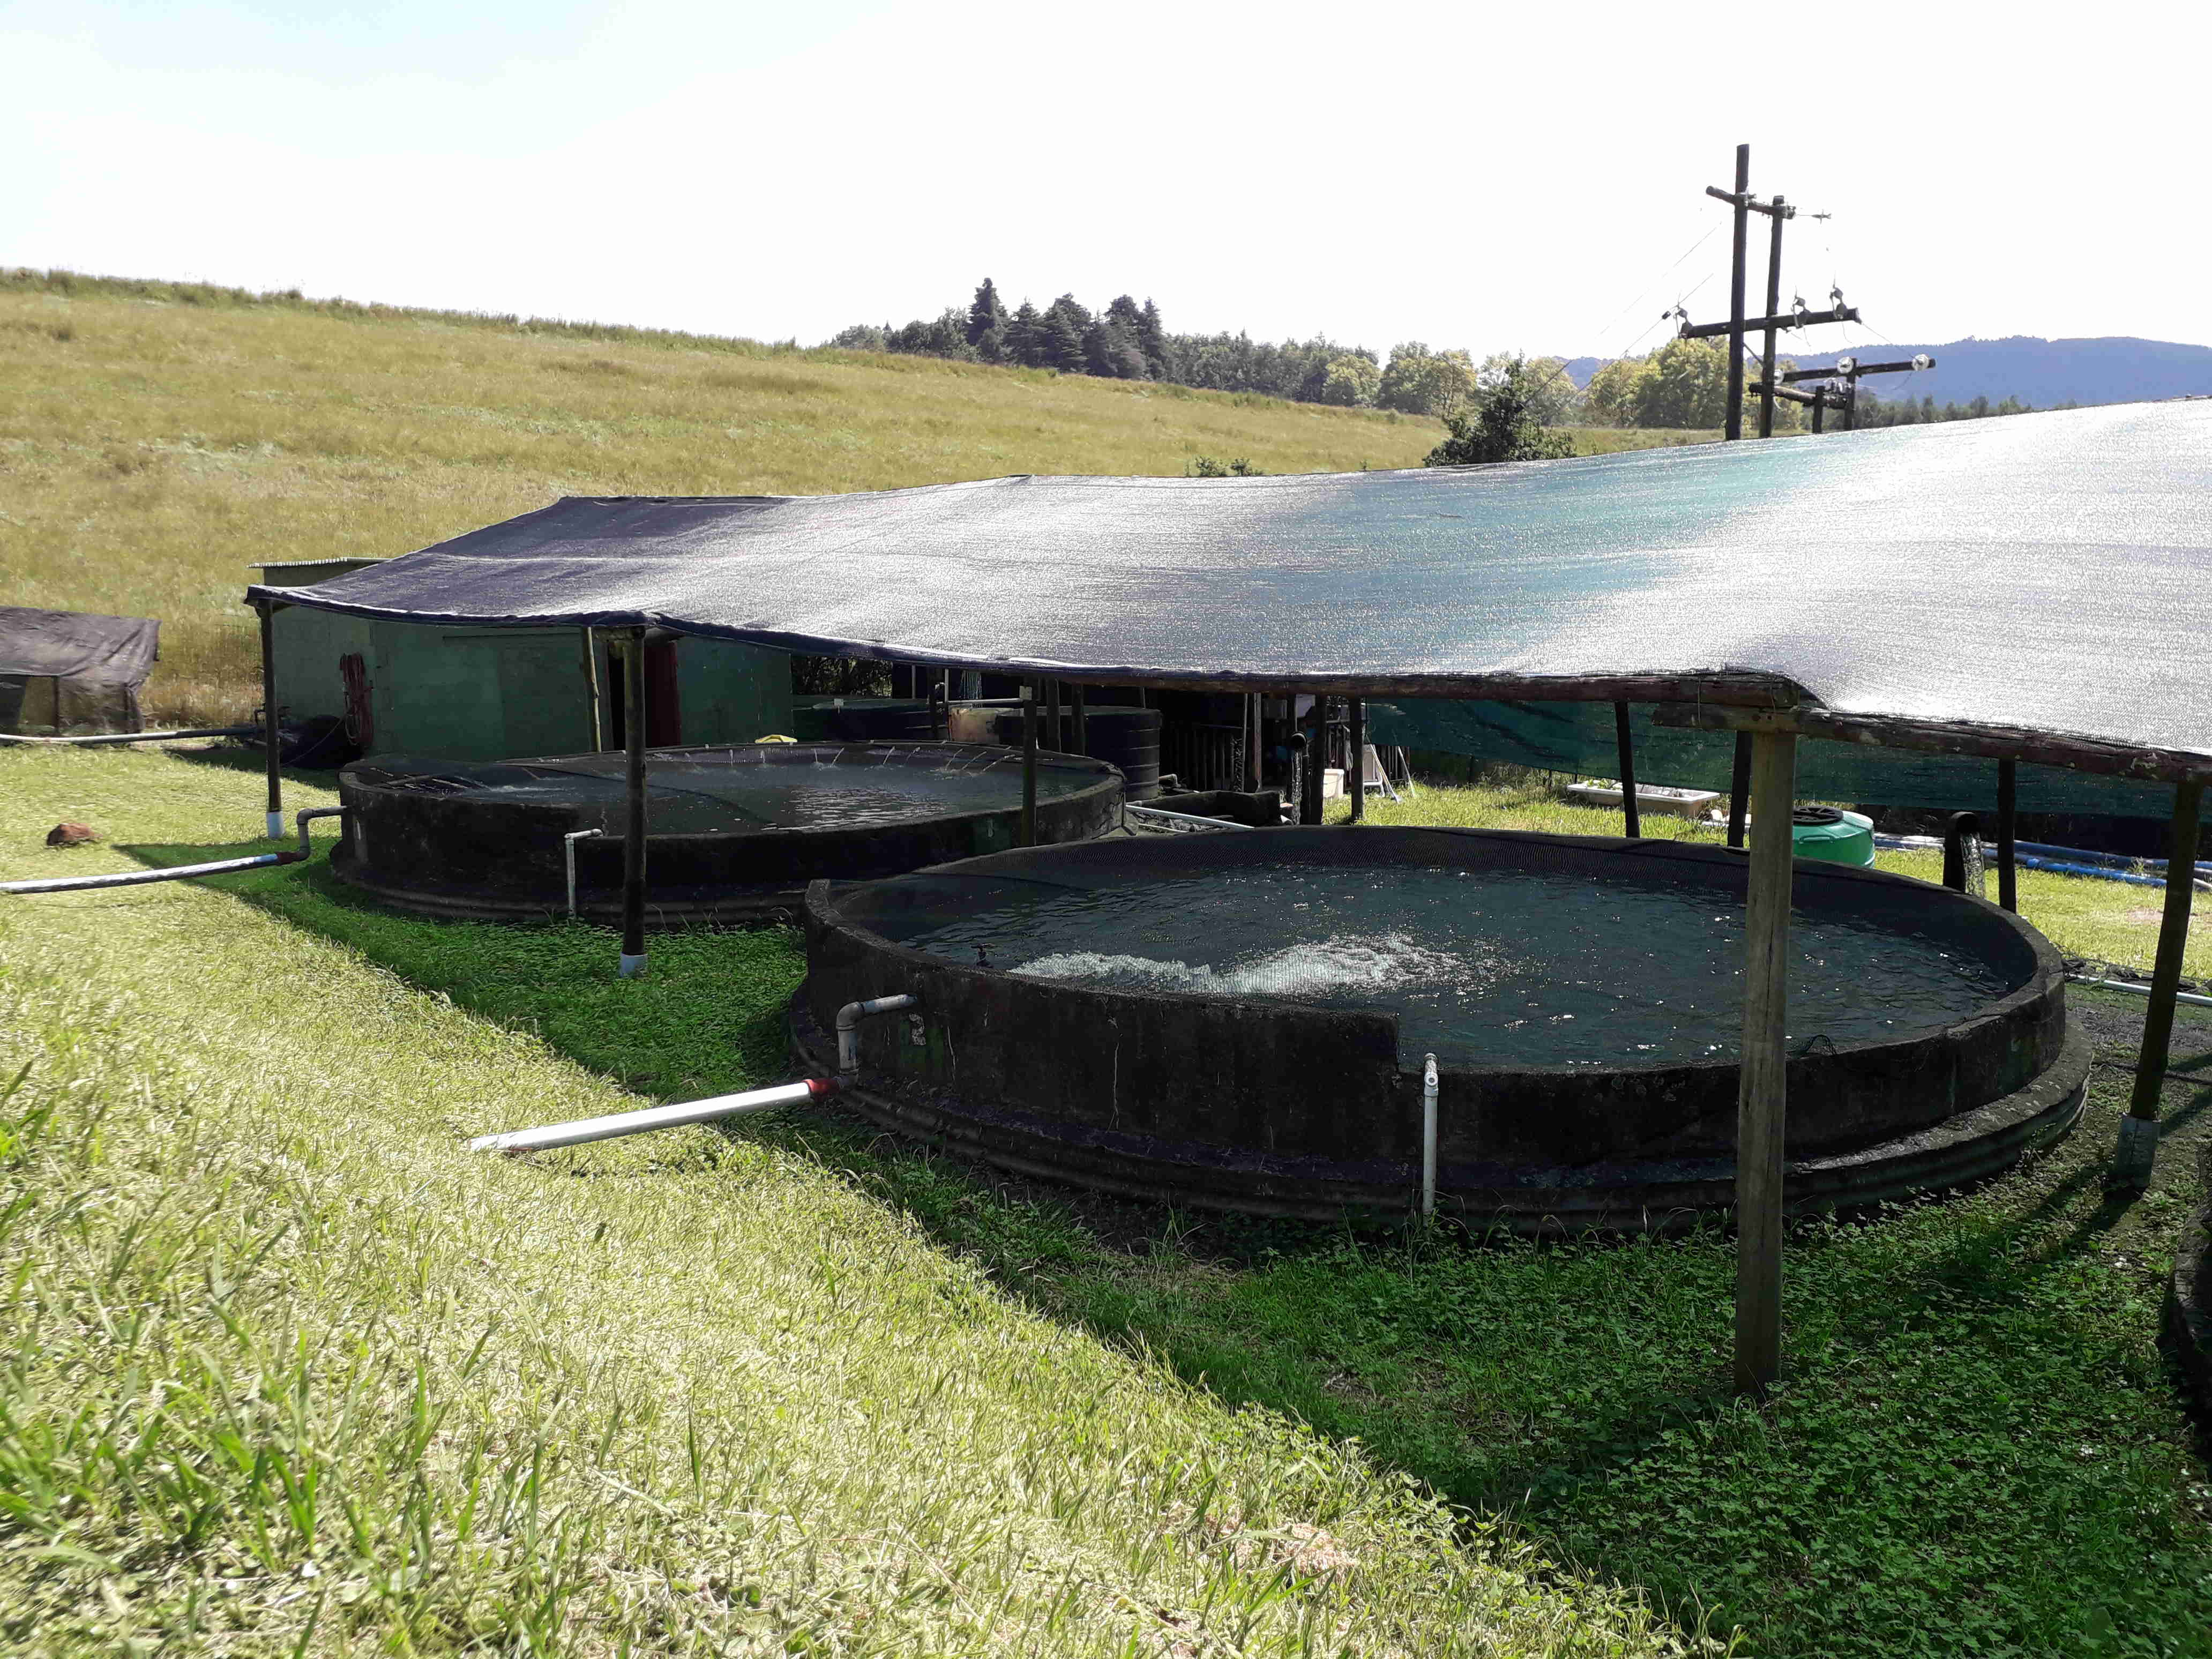
\includegraphics[scale = 0.1]{images/HatcheryPonds.jpg}
  \caption{Mbona growing ponds are of concrete construction and used for growing the fingerlings to sellable fish of length greater than 6 inches.  The flow rate through the pond is controlled by an inlet valve and the depth of water in the tank is determined by the height of the overflow outlet pipe. The ponds are covered with netting to prevent the fish from escaping. }
   \label{fig:HatcheryPonds}
\end{figure}



\subsection{Raceway}

\begin{figure}[H]
  \centering
   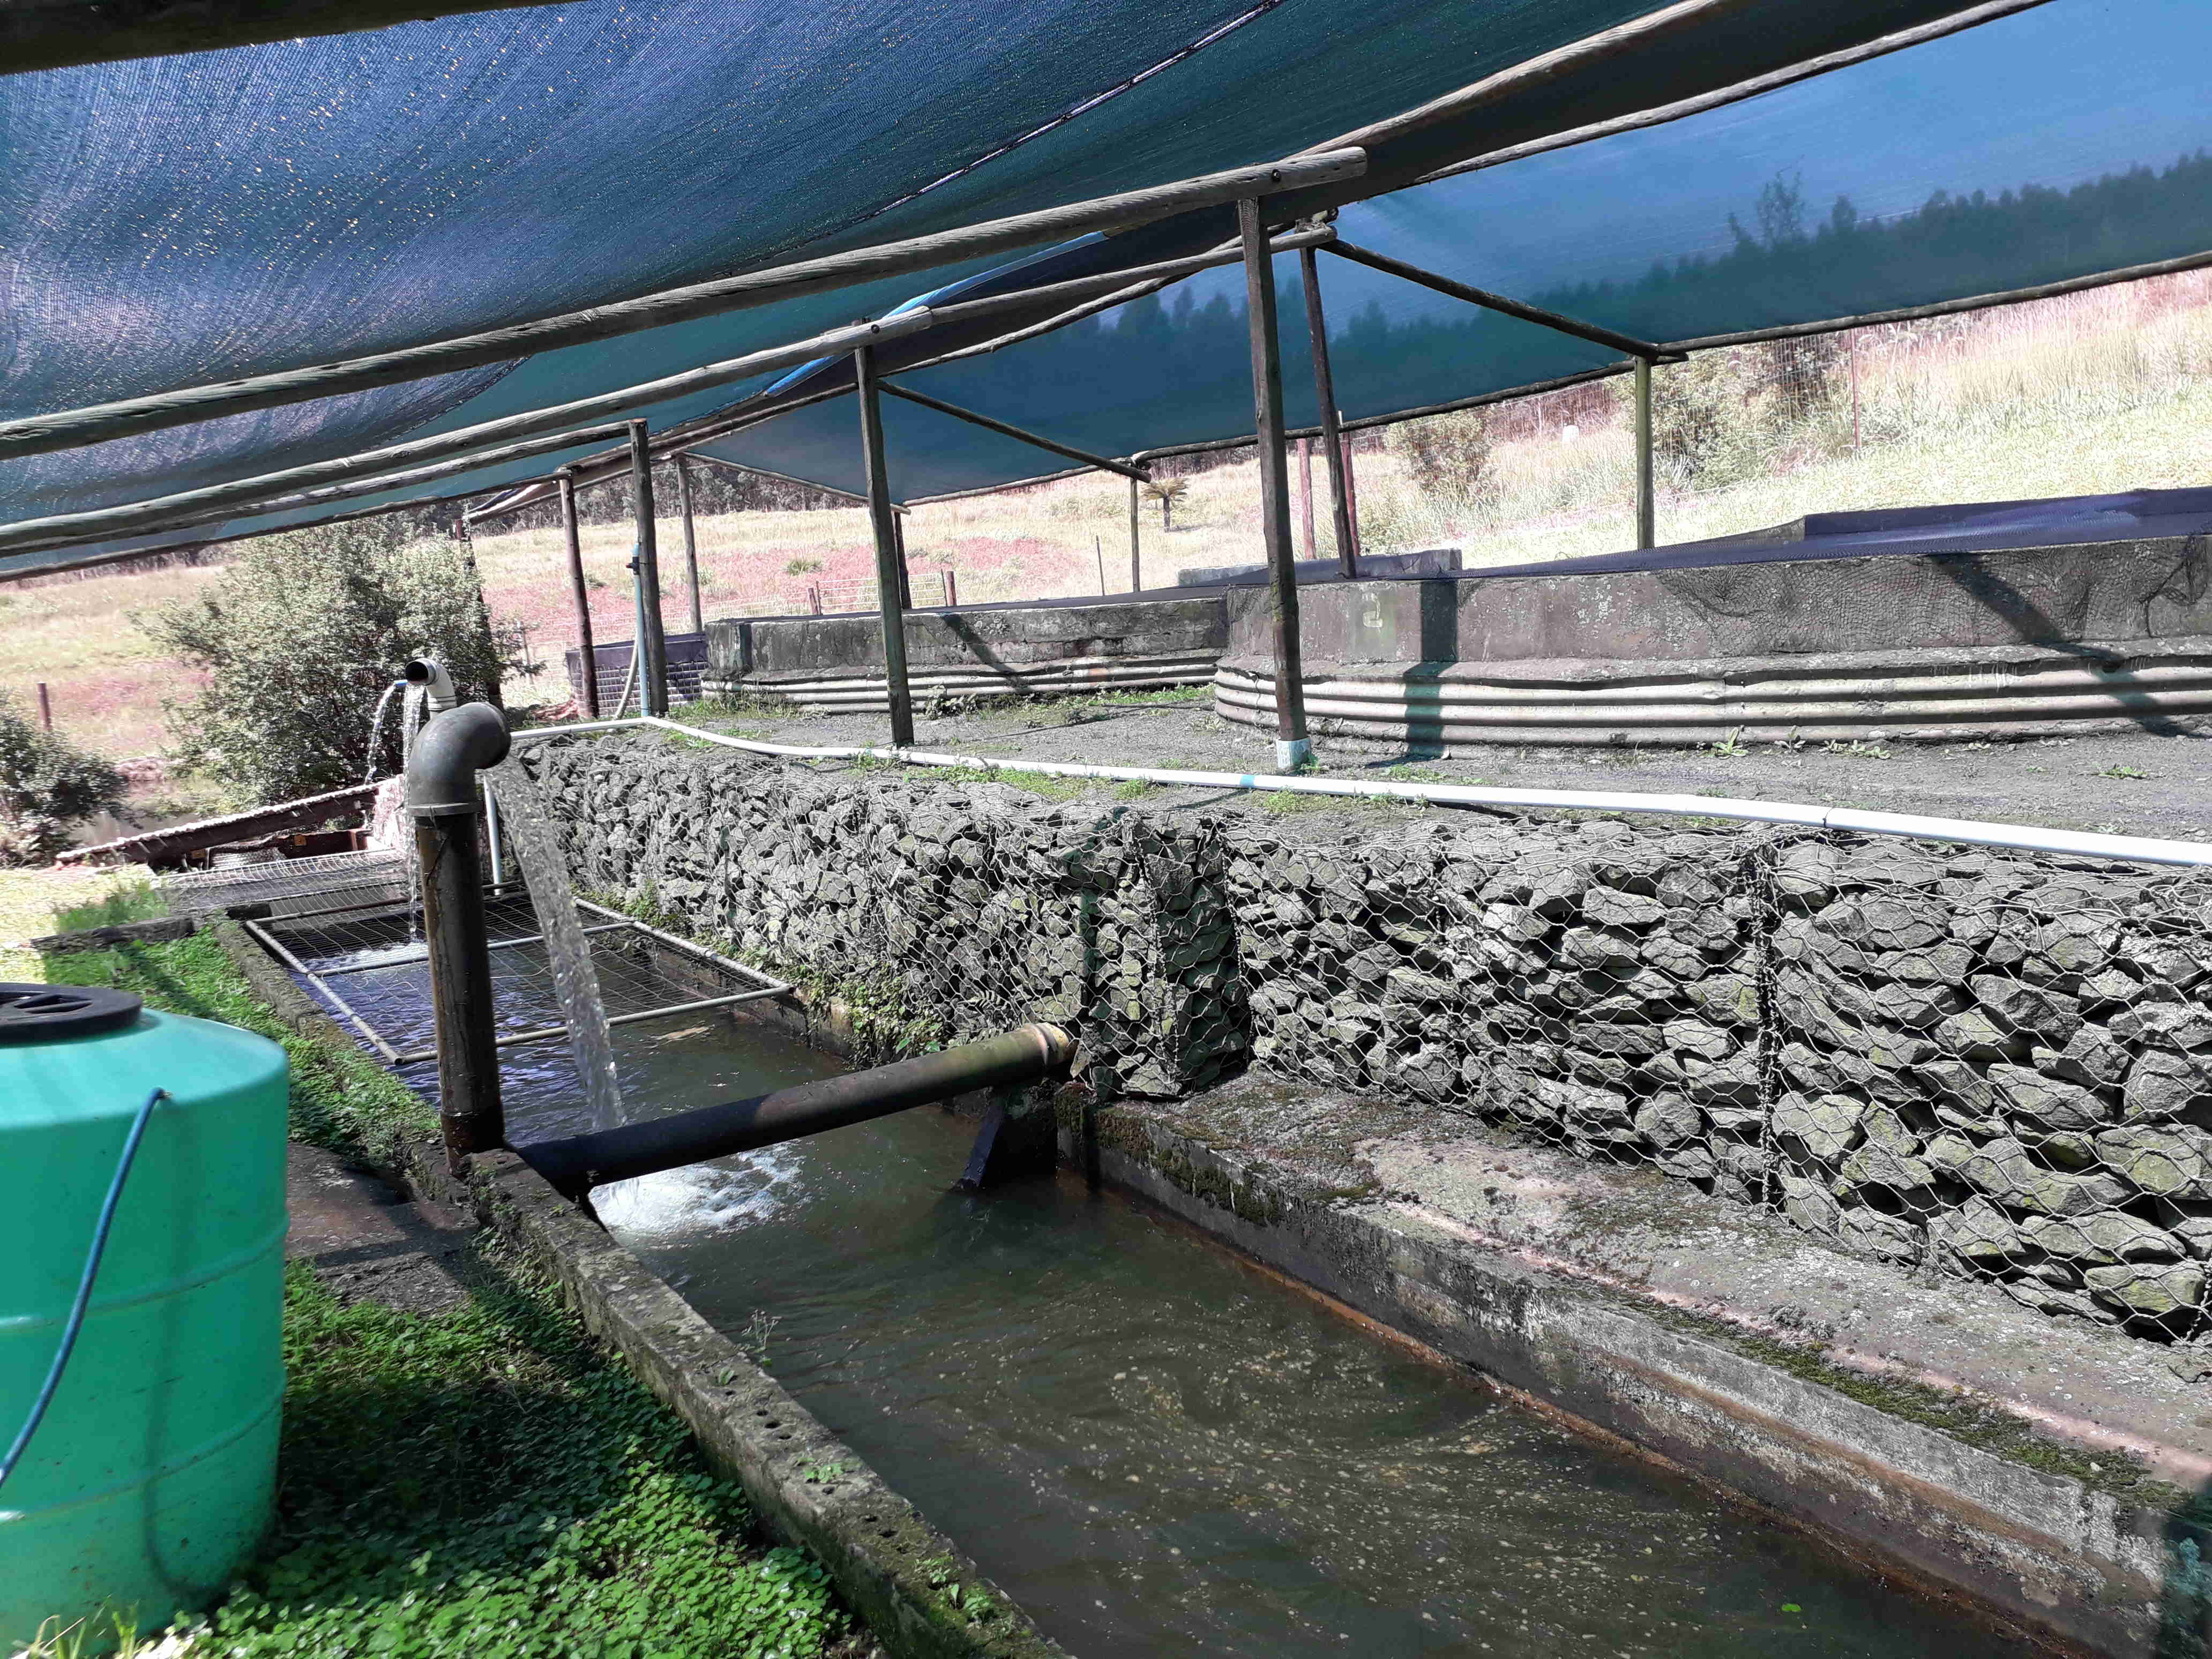
\includegraphics[scale = 0.1]{images/HatcheryRaceway.jpg}
  \caption{The Mbona raceway is used as an exit for the water after it has passed through the baths, tanks or ponds. It is also used to grow trophy and table fish for select customers.}
   \label{fig:HatcheryRaceway}
\end{figure}




\newpage
\section{Water Reticulation}

Water is siphoned from Lake Crystal and passed through an aeration tower before being piped to the baths, tanks, ponds and pools in the Mbona hatchery, see figure ~\ref{fig:HatcheriesWaterReticulation}. 

\begin{figure}[h]
  \centering
   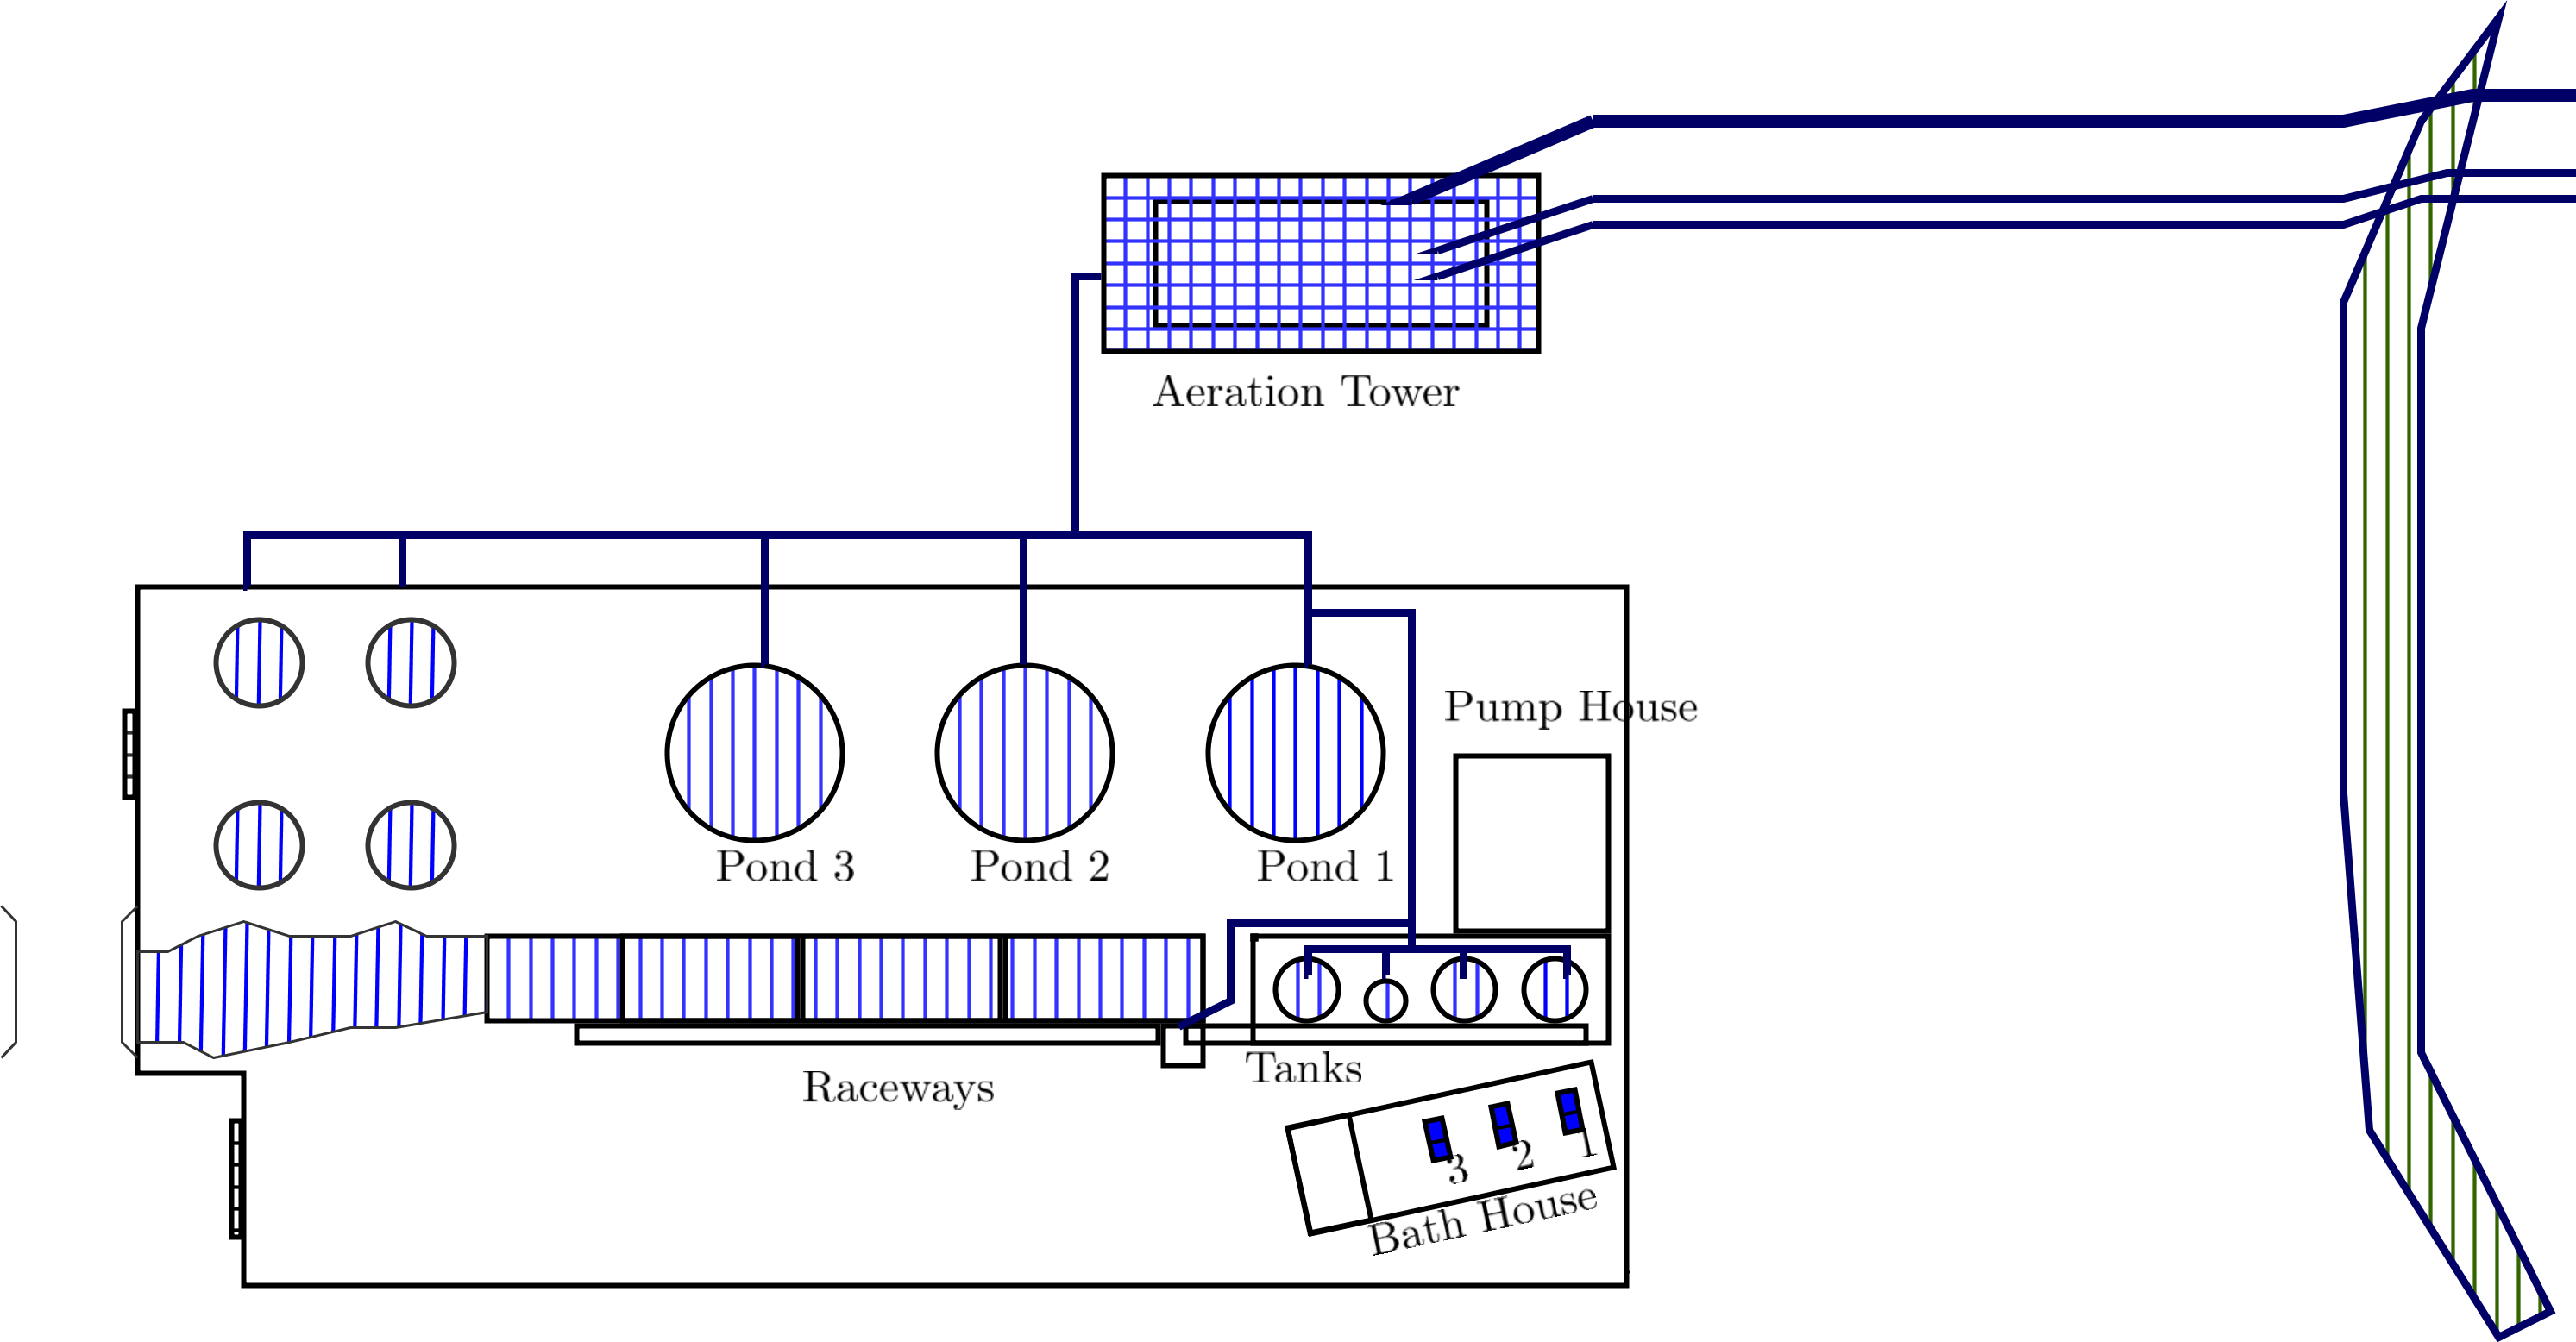
\includegraphics[scale = 0.15,angle=0,origin=c]{images/HatcheriesWaterReticulation.png}
  \caption{Mbona Hatcheries Water Reticulation System.}
   \label{fig:HatcheriesWaterReticulation}
\end{figure}

\subsection{Aeration Tower}

Aerated water is critical to the survival of live fish so The Mbona system used three different siphons to provide water to the aeration tower and on to the hatchery, see photgraph ~\ref{fig:HatcheryAerationTower}.

\begin{figure}[H]
  \centering
   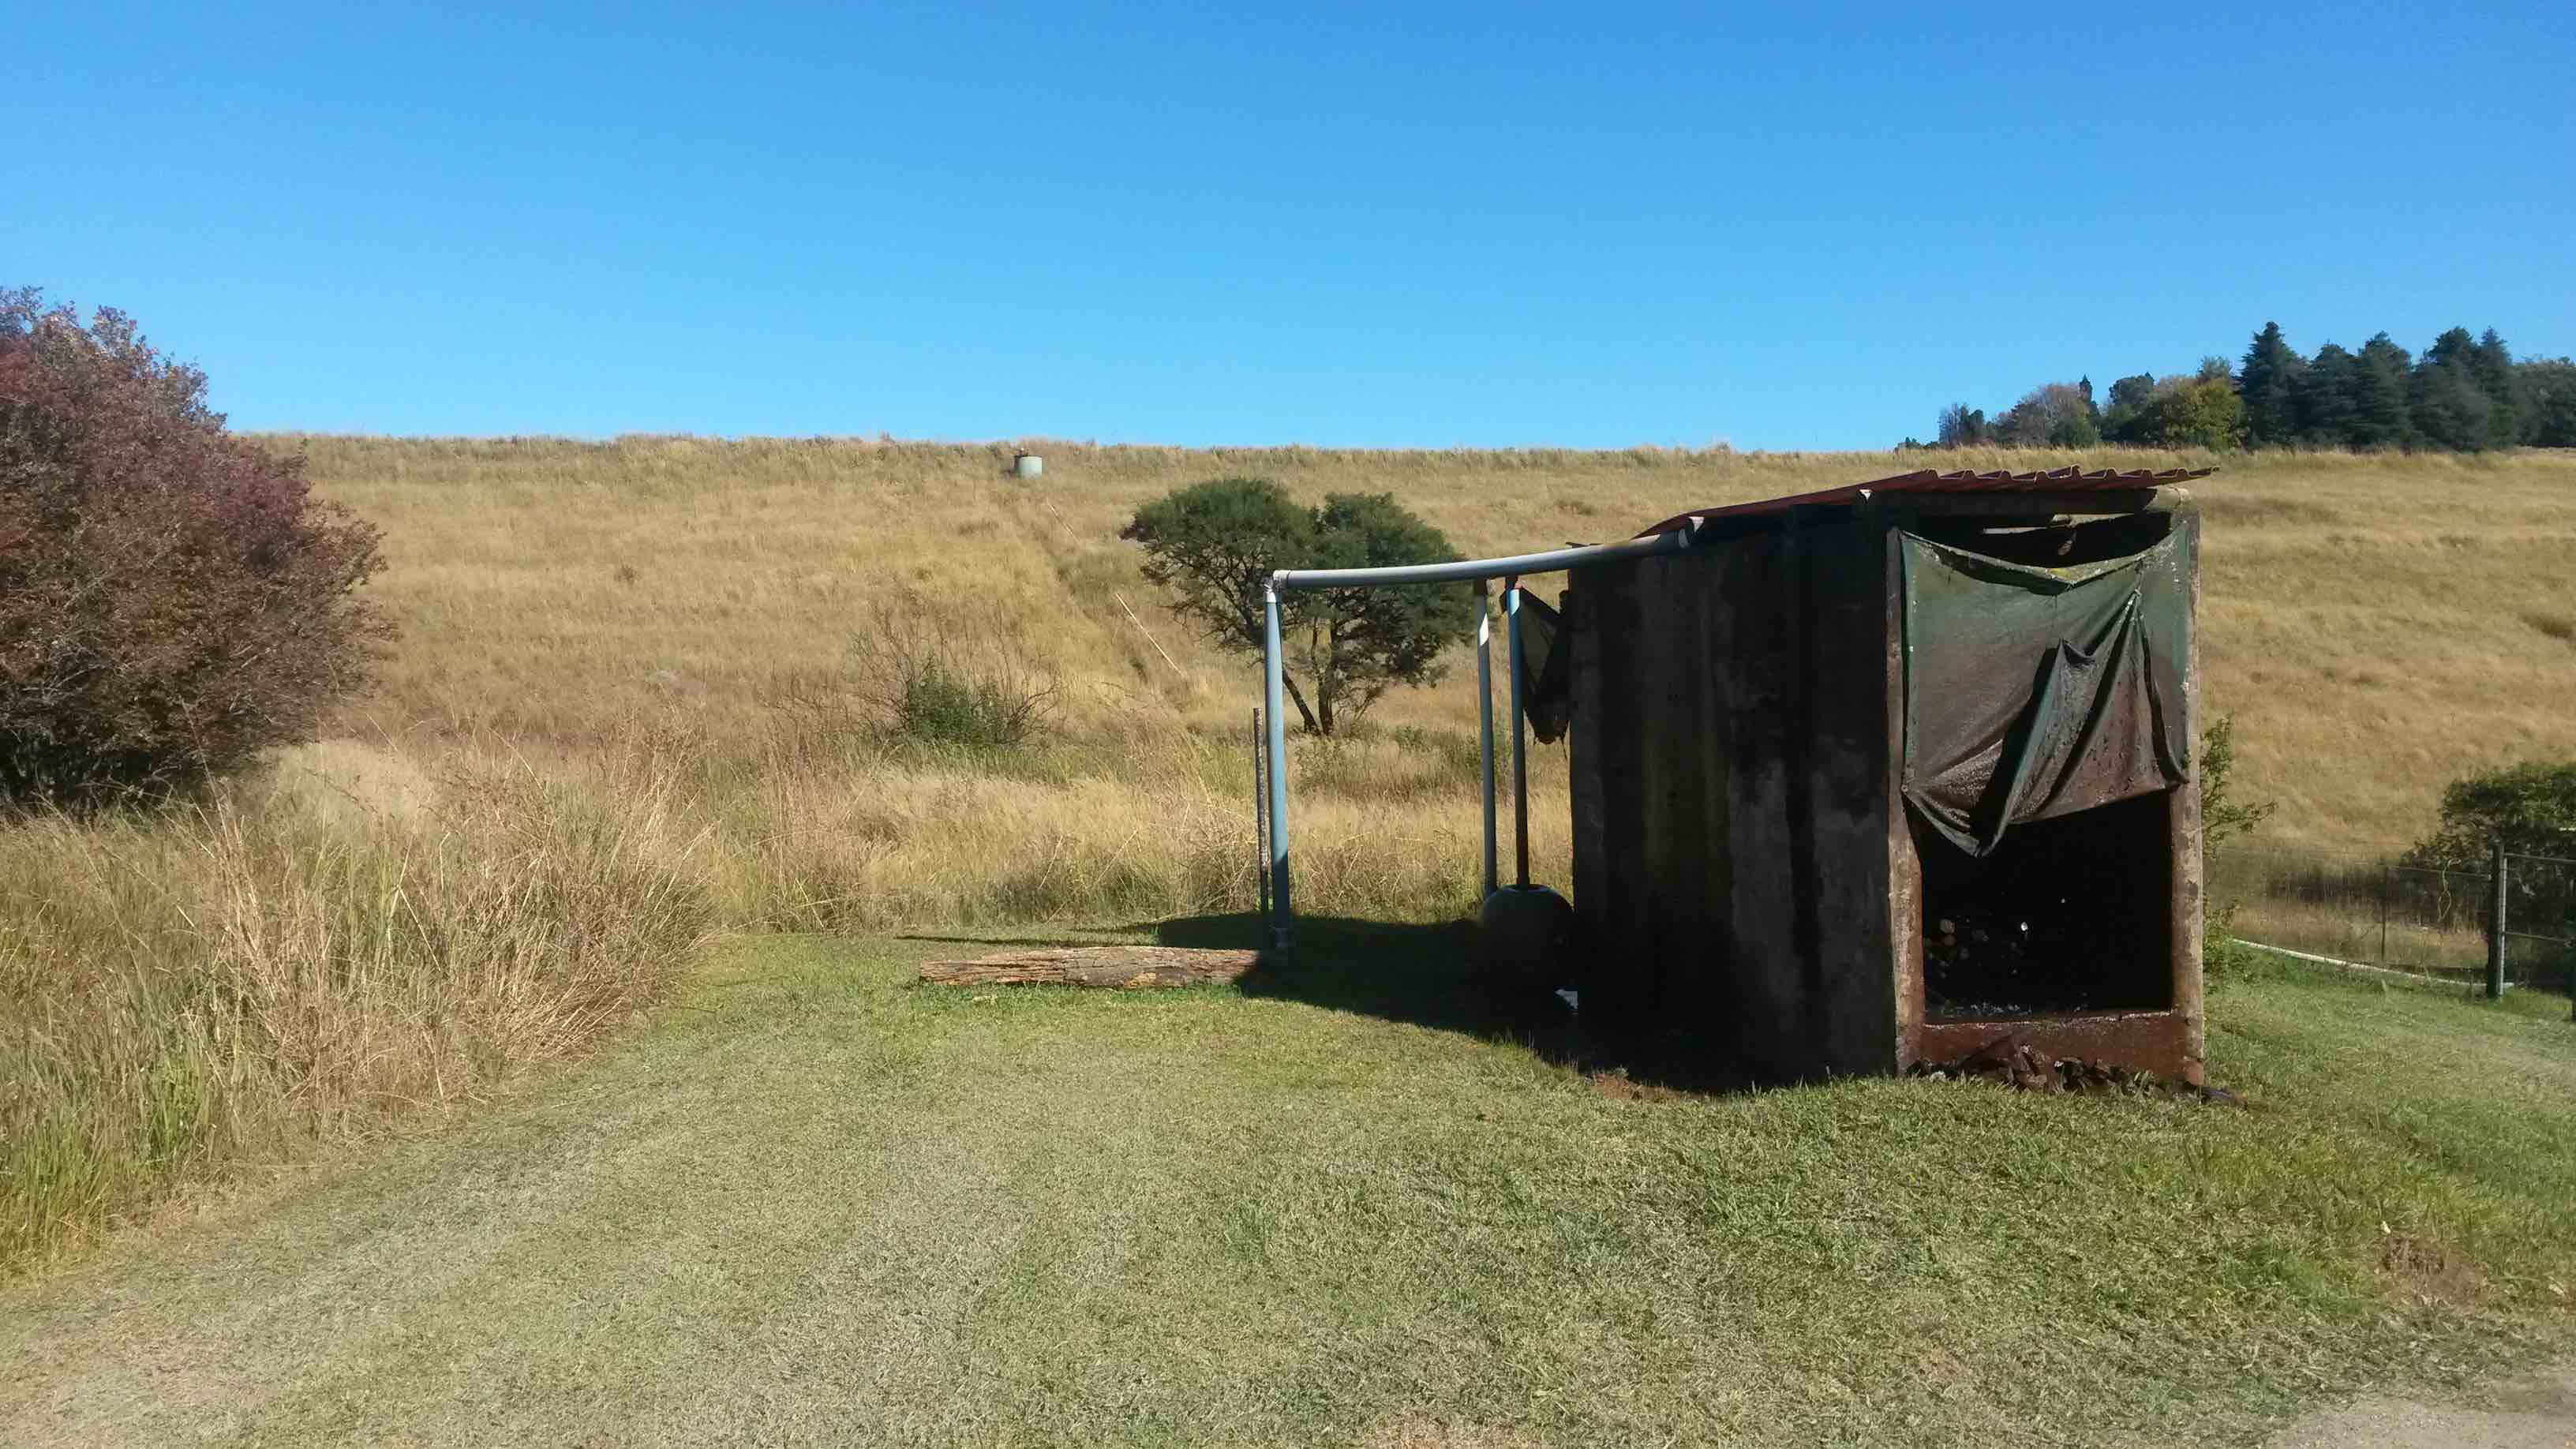
\includegraphics[scale = 0.1]{images/HatcheryAerationTower.jpg}
  \caption{The Mbona aeration tower is fed by {\bf three} siphons from Lake Crystal that must
  run continuously, see text for flow estimates.}
   \label{fig:HatcheryAerationTower}
\end{figure}


The flow of water from the three siphons can be computed using a formula outlined in the appendix of {\bf WaterPAK}, an Australian manual on best practices for the irrigation of cotton fields, see \cite{waterpak}.

The formula is based on Bernoulli's principle but adjusted for velocity loss due to friction between the water and the pipe. The flow rate for a siphon can be approximated by:

$$ Q = \frac{\pi D^2}{4} \sqrt{\frac{2 D H}{ 1.9 + 0.019 \frac{L}{D}} } $$

where

\begin{itemize}

\item[$Q$] is the flow rate in $m^3 s^{-1}$
\item[$D$] is the diameter of the siphon pipe in $m$
\item[$H$] is the height differential between the outlet and the lake surface in $m$.
\item[$L$] is the length of the siphon pipe in $m$.

\end{itemize}

Using this formula we compute daily discharge in litres expected from each of the 3 siphon pipes leading to the aeration tower. The results are presented in table ~\ref{tab:TablesSiphonVolume}.

\begin{table}[H]
  \centering
   
\includegraphics[scale = 0.8]{tables/TablesSiphonVolume.pdf}
   \caption{Siphon discharge in litres per day}
   \label{tab:TablesSiphonVolume}
\end{table}

These figures are supported by an experiment Pierre carried out when he use a bucket and stop watch to estimate the total consumption of the Hatchery with just the two smaller siphons feeding the aeration tower.
The results of this experiment are presented in table ~\ref{tab:TablesWaterConsumption}.

\begin{table}[H]
  \centering
   
\includegraphics[scale = 0.8]{tables/TablesWaterConsumption.pdf}
   \caption{Water consumption in the Hatchery as measured with a bucket and stopwatch.}
   \label{tab:TablesWaterConsumption}
\end{table}








\chapter{Mbona Hatcheries Procedures}

\section{Procedures}

%\subsection{Production Schedule, with TimeLine.}

In this section we track the progress of trout from eyed-eggs to fry to fingerlings, see figure ~\ref{fig:EggsFryFingerlings}.

\begin{figure}[H]
  \centering
   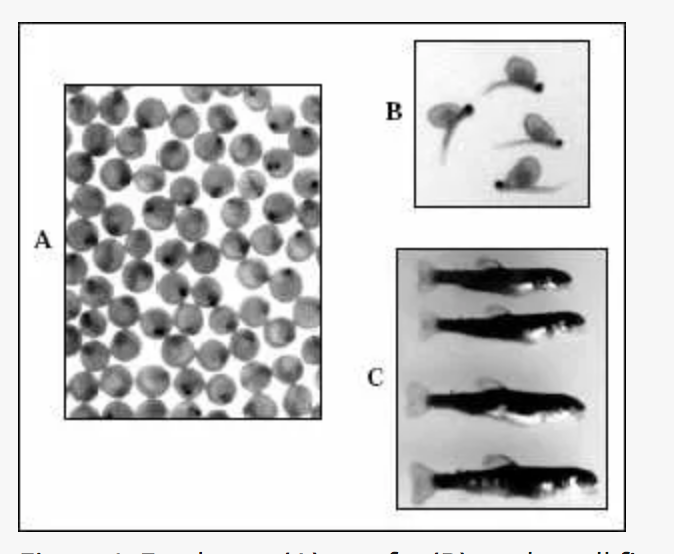
\includegraphics[scale = 0.6]{images/EggsFryFingerlings.png}
  \caption{What to look for: A) Eyed-Eggs, B) Sac-Fry, C) Fingerlings}
   \label{fig:EggsFryFingerlings}
\end{figure}

After this they spend the rest of their time in in the hatchery ponds as pre-sale growing fish.
In what follows we track the trout from Haching to sale giving feeding and cleaning schedules 
that must be followed.

\subsection{Preparation of Hatchery for new batch of eggs}

Make sure the fish food store is replenished. Purchase replacements from AVI feeds in Pinetown, 
see contact details ~\ref{tab:SupplierContactDetails}, who will deliver to Hopewell in Howick.
The current food range is outlined in the feed table ~\ref{tab:TablesFishFood}. This table is
just a suggestion, The suppliers of the feed should be consulted for their recommendation.

\begin{table}[H]
  \centering
   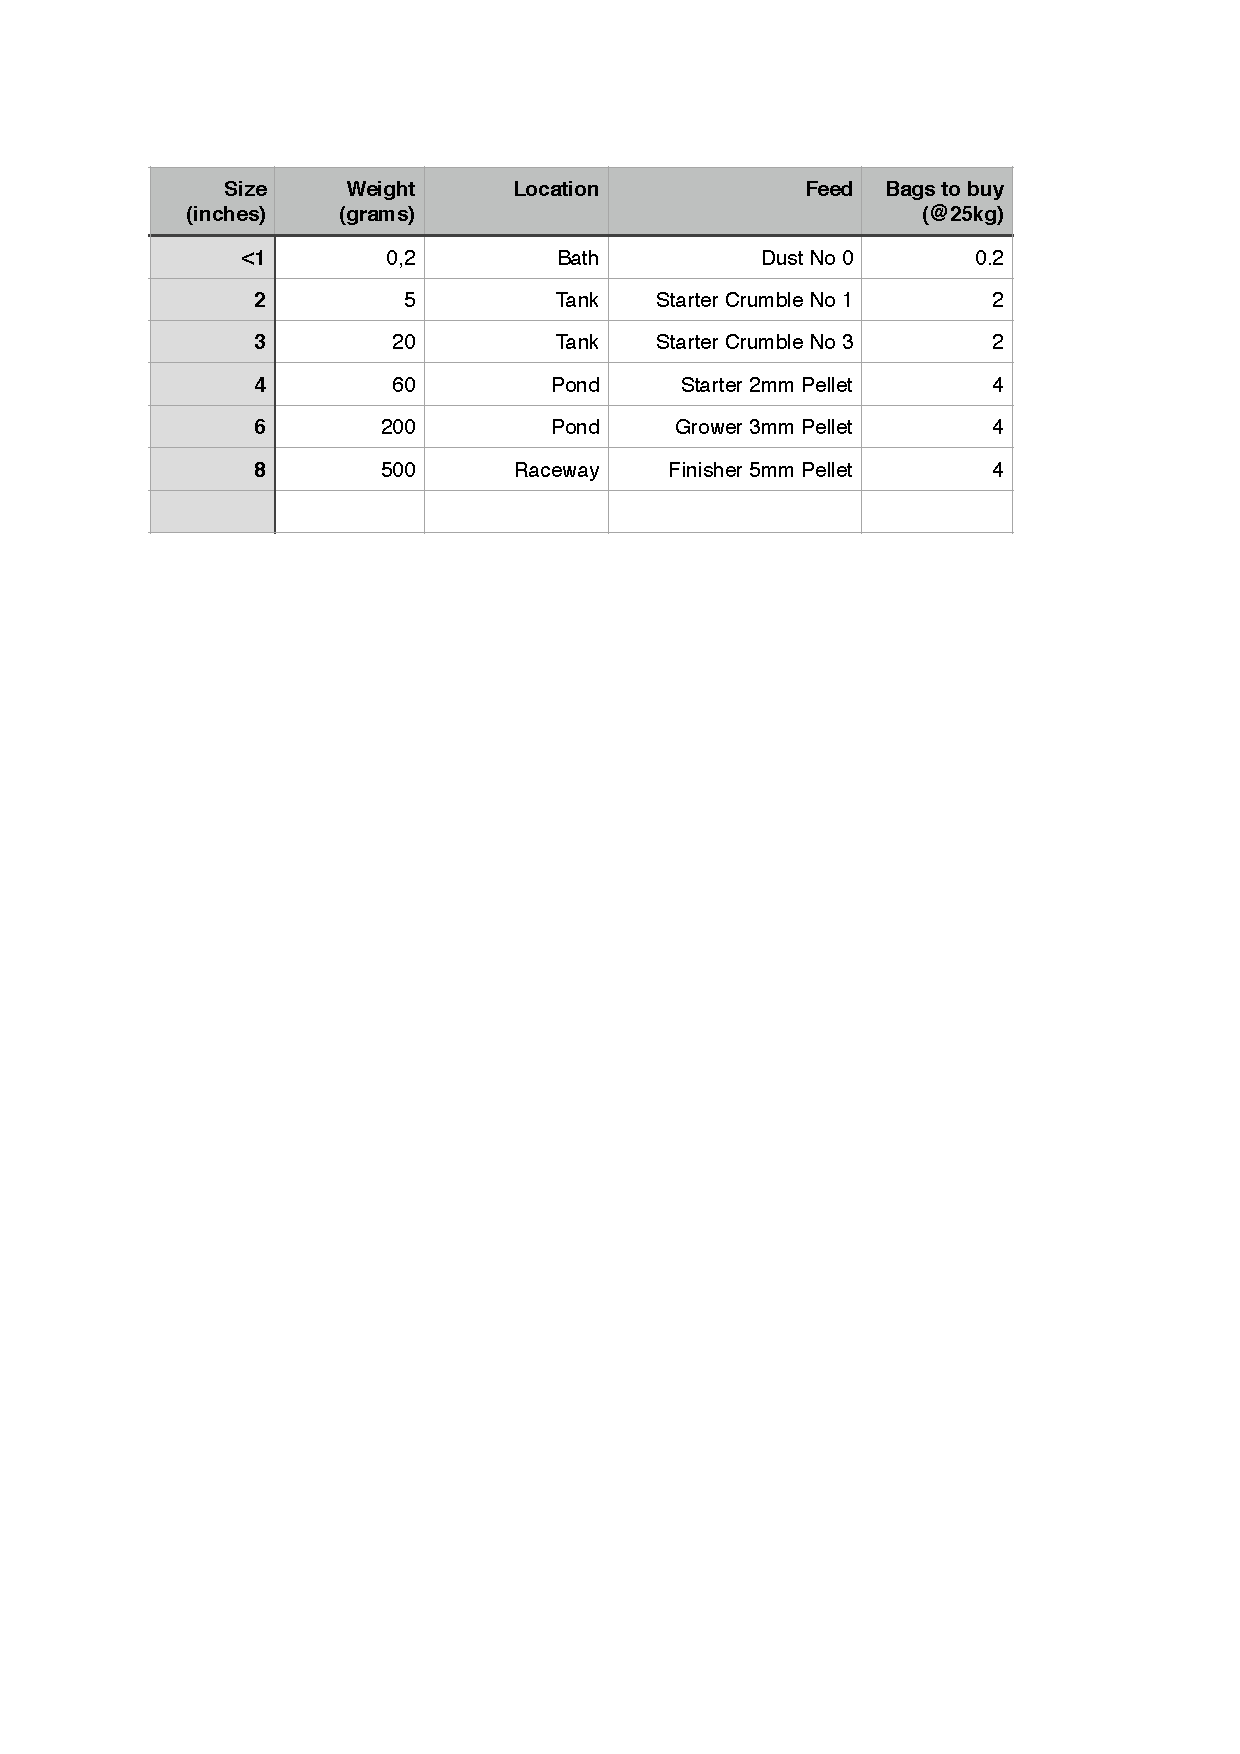
\includegraphics[scale = 0.9]{tables/TablesFishFood.pdf}
   \caption{Fish Feed: showing feed type to match different stages} 
   \label{tab:TablesFishFood}
\end{table}


Two weeks before the eggs arrive start with the following repairs and maintenance:  \marginpar{-2 \W}
\begin{itemize}
   \item Scrub three baths with abrasive pads \& Handy Andy
   \item Clean \& service in-feed pipes
   \item Clean \& service out-flow filters
   \item Check drain plugs \& safety locks
   \item Check \& repair mini vacuum cleaner
   \item Check the following equipment:
   \begin{itemize}
      \item 220 volt light globes in hatching room
      \item Roller blinds \& window covering
      \item Egg tweezers \& dead egg removal pipe \& bird feathers
      \item Head lamps \& batteries
      \item Digital scale
      \item Thermometers
      \item {\bf V} channel egg counter
      \item PVC gloves
      \item Egg transporting box
   \end{itemize}
\end{itemize}
   
Two or three days before arrival of eggs: \marginpar{-0.5 \W}
\begin{itemize}
   \item Scrub down all baths \& equipment again with Hibitane
   \item Position square egg trays in baths \& start water flow
\end{itemize}

On the day of collection \marginpar{0 \W}
\begin{itemize}
      \item Take egg transporting box, thermometer \& note pad.
      \item Buy ice in Howick, load transporting box \& pack spare ice in cool bag
\end{itemize}


\subsection{Transportation of eggs}

At the end of May about 10000 {\bf Eyed Eggs} are purchased from a Hatchery in 
Underberg, see the contact details table ~\ref{tab:SupplierContactDetails} .

Eggs are transported in a polystyrene box with trays of ice above and below the tray of eggs.
    The temperature in the box should be about  \SI{4}{\celsius}.

Eggs at  \SI{4}{\celsius} can be boxed for as long as 96 hrs (4 days).
The hatch-out-rate guarantee should be about 90\%.
The expected time to hatch out at  \SI{10}{\celsius} should be between 6 and 7 days.
    
Once the eggs have arrived at {\bf 0 \W} (weeks after arrival) they progress from 
hatching baths to fingerling tanks to fish ponds the schedule of which is outlined below:


\subsection{Egg handling on arrival}

On arrival at Mbona Hatcheries the eggs have to be tempered and  counted.
 \marginpar{0 \W \\ $1^{st}$June}

    
The tempering process requires increases the temperature of the eggs 
               to the temperature of the water in the incubation trays in a slow and regular manner. 
               The recomendation is  \SI{1}{\celsius} per hour.
               The temporing is accomplished as follows:
         \begin{itemize}
             \item[] Measure boxed eggs temperature.
             \item[] Half fill a bucket.
             \item[] Add ice or iced water to bring down bucket water temperature to egg temperature.
             \item[] When the two temperatures are equalised remove the ice from the bucket.
             \item[] Carefully add eggs to bucket and rehydrate eggs.
             \item[] Slowly bring the bucket temperature up to incubation tray temperature 
                        by adding small amounts of Mbona water from the baths to the bucket.
             \item[] aim for an increase of  \SI{1}{\celsius} per hour.
         \end{itemize}
         
Once the eggs have rehydrated the counting of the eggs can be accomplished by weighing a batch of 200 eggs, $W_B$, that are counted from a pharmacy tablet-counting device and then weighing the remaining eggs, $W_R$, in the rehydration bucket and computing the number of eggs received according to:
            
    $$ N_{eggs} = 200(1 + \frac{W_R} {W_B} ) $$
    
     In the past counting was done by the supplier in the presence of the customer so there was no need to recount on arrival at Mbona. 
     
     

\subsection{Hatching Bath Procedures}

  

\subsection{Hatching of Eyed Eggs}

Once the eggs have been transferred to the hatching trays they will take two weeks to hatch.
During this time white eggs (eggs that have died) must be removed from the hatching tray by
means of a suction straw. If this is not done regularly then the dead eggs will contaminate the live ones.  
\marginpar{2 \W}

After about two weeks, depending on water temperature, the eggs will hatch to produce sac-fry 
which will float away from the egg clutch and 
possibly spill out of the hatching tray into the hatching bath. These sac-fry will feed from their sac for another two weeks. 

After this the fry must be taught to feed. This is done by sprinkling food dust, see table ~\ref{tab:TablesFishFood}, on the water surface with a "plastic" water flow inhibitor in place
so that the food dust does not get expelled from the bath before the fry have fed.
\marginpar{4 \W}

In the beginning this feeding must occur at least {\bf SIX} times a day whilst the fry are still in the baths.
After 2 weeks of feeding the feeding rate can be reduced to {\bf FOUR} times a day for another 2 weeks.
Note that when the fry are young they must be fed small amounts and often so as to maintain equal growth rates amongst the fry and thus reduce canabalism. 

After feeding, some food dust will sink to the bottom of the bath and this sediment must be cleaned 
regularly by  vacuuming the bottom of the bath with the mini vacuum machine.
     
 \subsection{Relocation of fry from Baths to Tanks}
 
 As soon as the fry learn to feed by themselves the Tanks must be prepared to receive the fry.
 All four tanks must be cleaned with diluted Chlorhexiden Gluconate, (Hibitane). Read the 
 instructions to get the dilution proportions. 
 The sides of the tanks must be brushed and broomed and flushed repeatedly. 
 The water must be running a few days before the fish arrive. 
 \marginpar{6 \W}
 
 When the mortality rises in the Baths move the fry to tanks, 
 Use tanks 2 and 4 with {\bf runts} in tank 3.
 Use tank 1 for overflow from 2 and 4.
 Use buckets and the displacement method to count and record the number of fry moved.  
\marginpar{8 \W}

The fry will remain in the tanks for two months. During this time they must be fed with
 starter crumble, see the feed table ~\ref{tab:TablesFishFood}.

\begin{itemize}
          \item twice daily for 4 weeks using starter crumble no 1
          \item twice daily for 4 weeks using starter crumble no 3
\end{itemize} 

 The amount of food to feed can be estimated from the following entry in the 
 Trout in the Classroom website \cite{tic}.
 Assuming 1000 baby fish feed them approximately the following amount of food each day:

\begin{itemize}
\item fish starting to swim up: feed very little (use dust number 0).
\item fish just out of hatch box: 1.5 grams. (use dust number 0)
\item fish approx. 1 inch: 6 grams. (use starter crumble 1)
\item fish approx. 1.5 inch: 17 grams of food (use starter crumble 3).
\item fish approx. 2.25 inch: 55 grams of food (fish ready for transfer to ponds).
\end{itemize}


\subsection{Relocation of fingerlings from Tanks to Ponds}

1 week before the fry reach fingerling stage the ponds must be prepared to receive them.
Use the same technique to clean the ponds. Make sure the ponds are clean and water has
been running for at least two days before transferring the fingerlings.
\marginpar{15 \W}

    Use the gutters and count and transfer the fingerlings to the ponds.
    measure the average length using a 10\% sample of the fingerlings transfered.
    Transfer into pond 1 and 2 with overflow to pond 3   
    \marginpar{16 \W}
    
    
    feeding schedule, see the feed table ~\ref{tab:TablesFishFood}.
        \begin{itemize}
          \item twice daily for 4 weeks using 2mm pellets
          \item twice daily for 4 weeks using 3mm pellets
          \end{itemize}
     after this the fish are ready to move to dams 
     \marginpar{24 \W}

\subsection{Feeding Schedule for growing fish}

When the fish are in the ponds they should be fed according to their total weight per day.
Assuming optimal temperatures between \SI{12}{\celsius} and \SI{18}{\celsius}, they should be fed
$2.5\%$ of their body mass. This amount should be split in two and the growing fish should be fed twice daily.

Below \SI{10}{\celsius} the daily food allowance should be droped to $1.5\%$ of total body mass and below
\SI{5}{\celsius} it should be reduced further to $1\%$ of body mass.

Above \SI{20}{\celsius} the daily food allowance should also be reduced since at this temperature the fish become too lethargic to feed.

The weight, $W$, of a fish can be estimated from its length and girth as follows

\begin{itemize}

\item[] {\bf Imperial} $W$ in pounds, $L$ and $G$ in inches:
$ W  = \frac{1}{800} \times L  \times G^2 $

\item[] {\bf Metric} $W$ in grams, $L$ and $G$ in centimetres.
$ W  =   \frac{450}{800} \times L  \times G^2 $

\end{itemize}

In table ~\ref{tab:TablesWeightComputation} you will find example computations for various fish dimensions

\begin{table}[H]
  \centering
   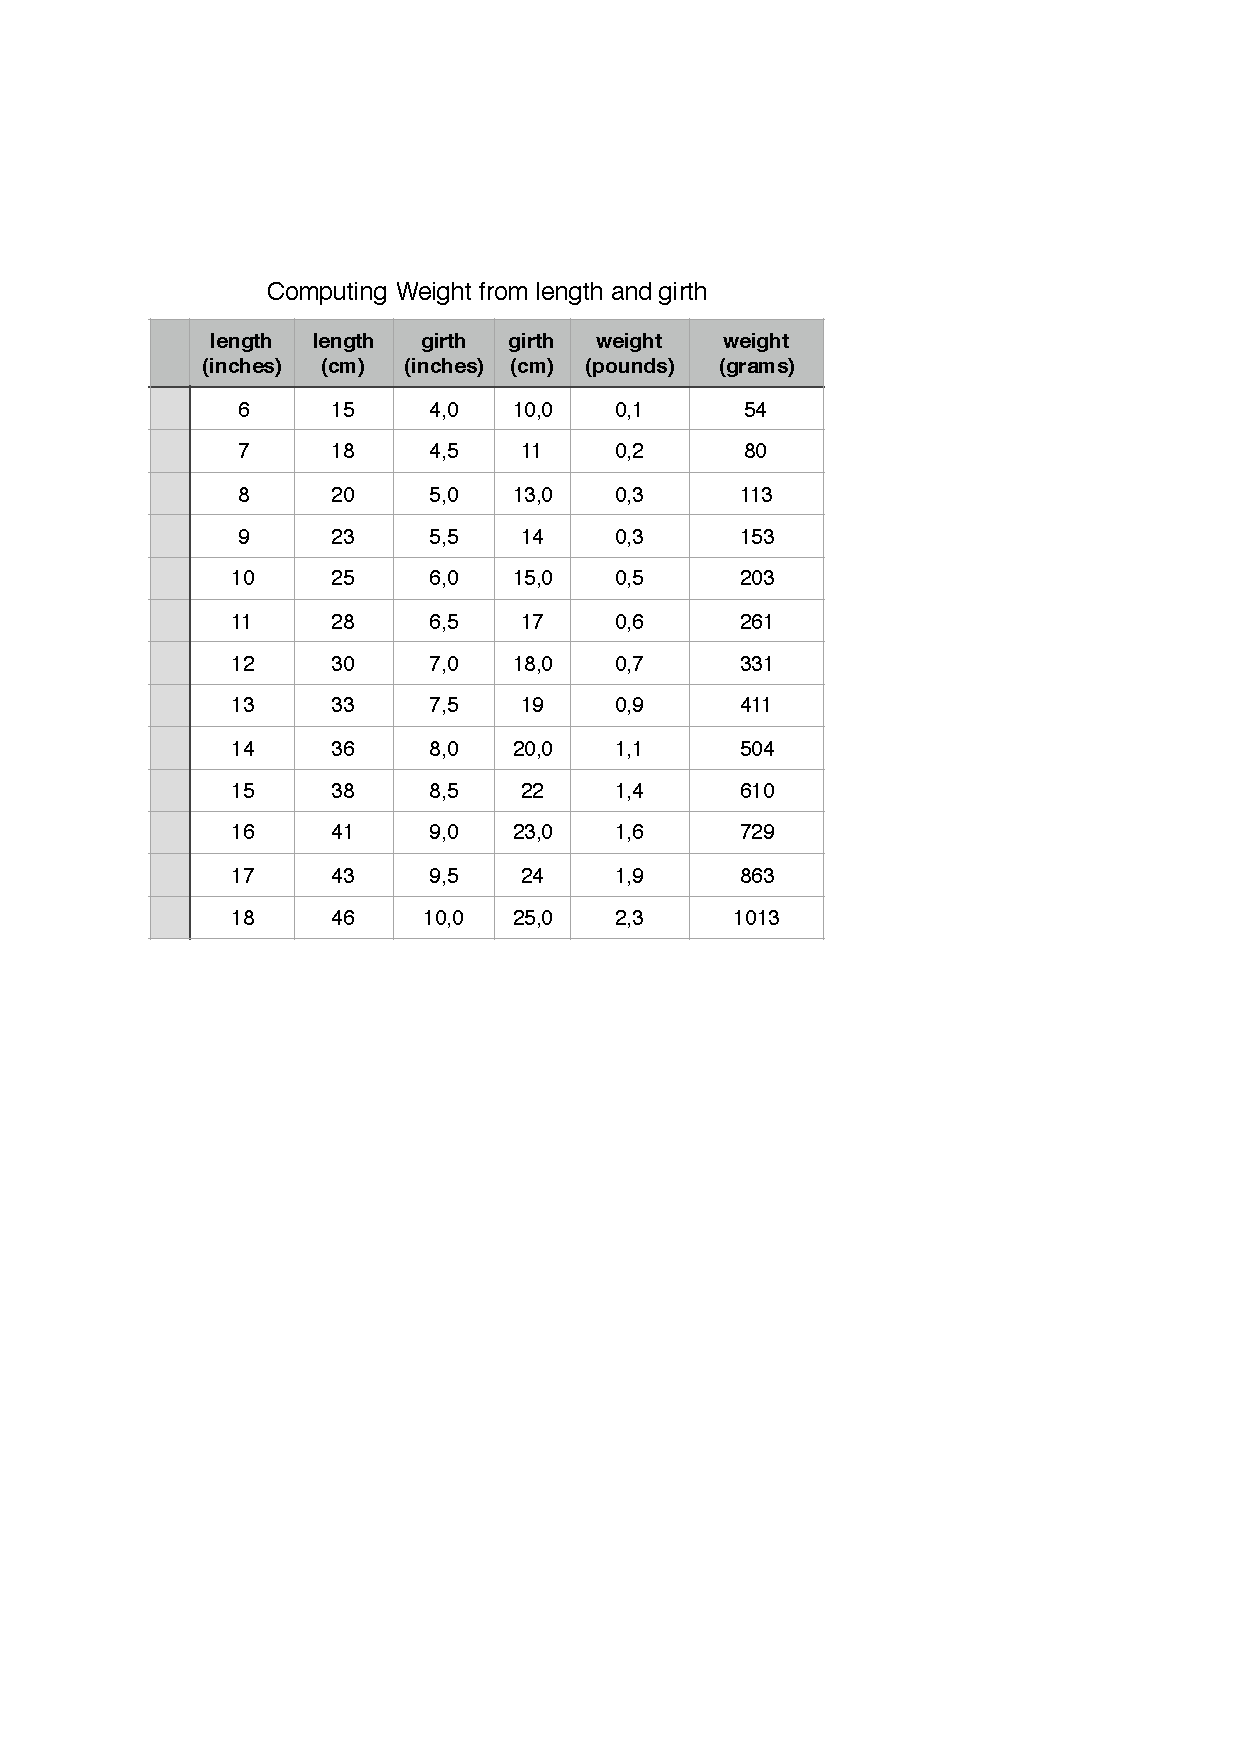
\includegraphics[scale = 0.8]{tables/TablesWeightComputation.pdf}
   \caption{Computing weight from length and girth, $W \approx L \times G^2$}
   \label{tab:TablesWeightComputation}
\end{table}




\subsection{Moving Stock Fish to Dams}
   
    When the fish in the ponds reach an average length of 6 to 7 inches they are ready to
    be sold to customers or used to restock Mbona dams. Customers must be contacted
    timeously so that orders can be taken and expected delivery dates agreed upon and 
    the fishing committee must meet to decide on which dams are to be restocked.
    
    Prices for live fish are set annually. Since the Mbona operation is {\bf non-profit}, prices
    are kept just below market value and sales are limited so that Mbona can stock their
    own dams adequately. Current prices are shown in table ~\ref{tab:TablesFishPrices}.
    
    \begin{table}[H]
  \centering
   
\includegraphics[scale = 0.8]{tables/TablesFishPrices.pdf}
   \caption{Selling Price for Mbona Fish, the six inch price is set annually and
   the price of the larger fish increases 10\% per inch and the price per fish is
   rounded to the nearest rand.}
   \label{tab:TablesFishPrices}
\end{table}
    
    Stock fish are counted and transported using a 600 litre tank mounted on 
    an Mbona Isuzu with oxygenator attached.  The number of fish the tank can  
    accommodate depends on the average size of the fish as outlined in the table ~\ref{tab:TransportationNumbers}.
    
    \begin{table}[h]
  \centering
  \begin{tabular}{|c|c|}
    \hline
    length & number   \\ \hline
    7 inch & 700  \\ \hline
     8 inch & 400  \\ \hline
      9 inch & 300  \\ \hline
       10 inch & 250  \\ \hline
  \end{tabular} 
  \caption{Numbers versus Length for 600 litre vessel.}
  \label{tab:TransportationNumbers}
\end{table}

Live fish that are not sold are used to stock the Mbona dams. The number of live fish a dam can support
depends on the surface area of the dam and the size of the fish. In table ~\ref{tab:TablesDamCapacity} we
show dam capacities for a range of fish sizes. In the last column we show suggested proportional stocking
figures assuming 1000 fish were available for dam stocking. Naturally these numbers are not cast in stone
as dams may not be in a fit condition to receive stock fish. For example,Holbeck may be silted up and
Emerald may be empty.

\begin{table}[H]
  \centering
   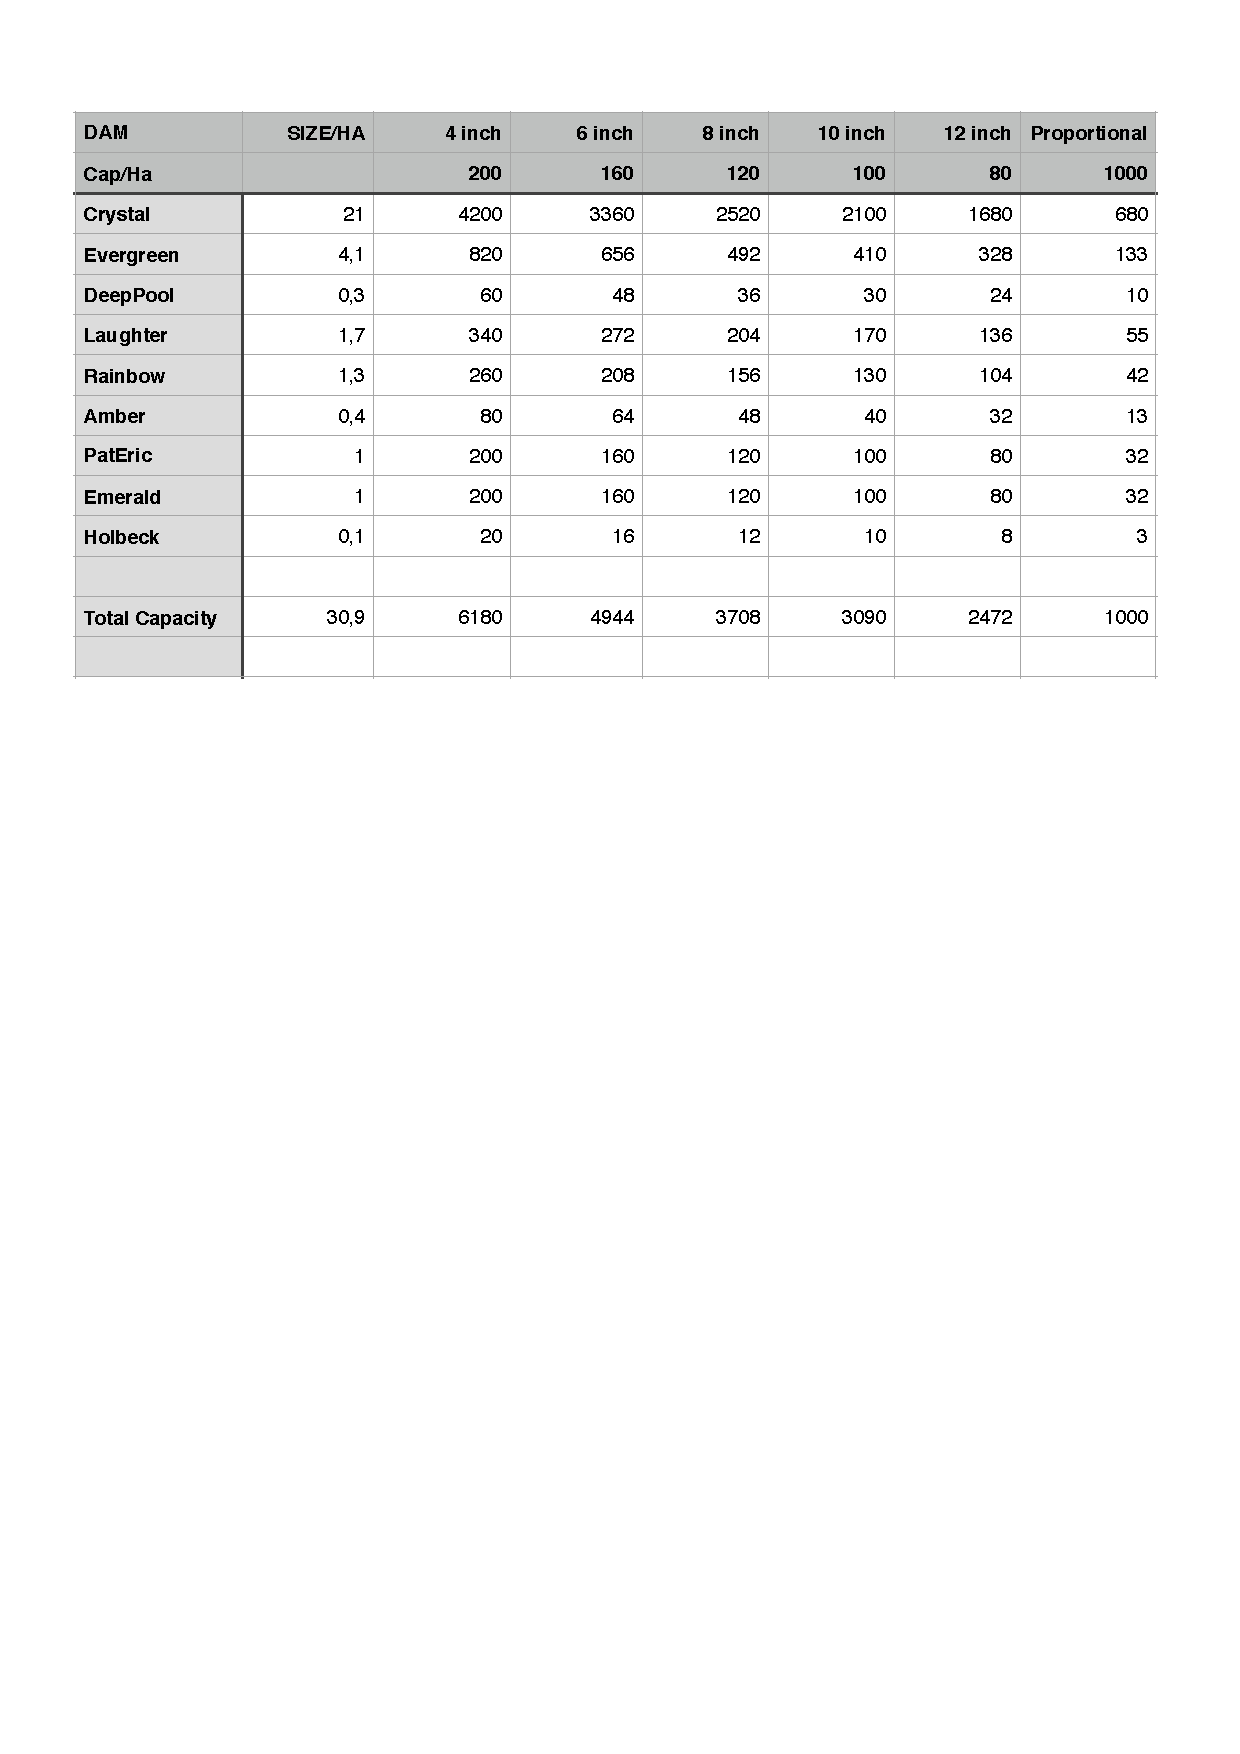
\includegraphics[scale = 0.7]{tables/TablesDamCapacity.pdf}
   \caption{Dam Capacities on Mbona, Each column shows the dam capacities dependent on
   the current size of the stock fish. The last column shows suggested proportional allocation
   assuming 1000 stock fish are available}
   \label{tab:TablesDamCapacity}
\end{table}



\subsection{Hatchery Staff Duties}

\subsubsection{In preparation for egg arrival}

\begin{itemize}
\item When informed of a pending fish delivery, lay out \& check \& clean all delivery equipment.
\item Pack all fish transporting equipment way after use 
\item Report any damaged or lost equipment to management.
\end{itemize}


\subsubsection{During Incubation and sac-fry growth}

\begin{itemize}
\item remove white eggs {\bf three} times per day.
\item make sure baths are clean, just sweep in preparation for hatching.
\item when teaching fry to eat, use very small amounts of dust and fry must be seen breaking the water surface when feeding.
\item Baths must be vacumed a half hour after each feed.
\end{itemize}

\subsubsection{During Growth Period}

\begin{itemize}
\item Feed fish daily according to Size - Quantity - frequency chart.
\item Vacuum clean tanks and ponds after each feed.
\item Keep pond nets in good repair
\item Inspect all fencing \& keep grass cut under \& around electric fence.
\item Keep large \& small catch nets in good repair.
\item Cut grass and keep hatchery area \& hatchery room neat \& tidy at all times.
\item All long catch net \& vacuum poles to be cleaned \& stored on racks
\end{itemize}

\subsubsection{At all times}

\begin{itemize}
\item Keep all fish transporting equipment clean \& stored under cover 
\item Report any broken or damaged equipment to management same day.
\item Report any predator activity, otter or birds of prey, to management same day.
\end{itemize}





\newpage
\section{Mbona Hatcheries Maintenance and Repair}

Maintainance and repair projects as of March 2019 (completed projects marked \checkmark).

\subsection{Hatching room}     

\begin{itemize}
\item Repair bath 2 in-feed pipe
\item Make good all three bath outlets and make adjustable drains. 
\item Make 3 PVC/F-glass mesh filter curtains  
\item Stop leaks in drain out-pipes
\item Sort 220v lighting in hatching room
\end{itemize}

\subsection{Main pond area}     
\begin{itemize}
\item Complete clay repair and gravel of raceway pond.    
\item Complete fencing and gates to new extension   \checkmark
\item Reroute electric fencing \checkmark
\item Run water feed pipe to new area off main 3 pond feed \checkmark
\item Replace small fingerling tank with larger model.
\end{itemize}

\subsection{Shade cloth cover}  
\begin{itemize}
\item Replace and reset gum poles  \checkmark
\item Replace shadecloth \checkmark 
\item Replace swimming pool hose sections where necessary \checkmark
\item Build, using old fencing standards, adjustable drain pipe stands
\item Do 12 volt night light bug catch test with white plastic \checkmark (not successful)
\end{itemize}


\subsection{Syphon water feed from Crystal}
\begin{itemize}
\item  Pull up 2 x 70mm syphon pipes and replace filters \checkmark
\item Move 3 syphon inlets and main water inlet 18 meters further from wall
\item Build mud anchor and substantial top float with nylon rope-pulley lifting system for maintenance.
\item Box and cover 3 x vacuum break valves at Crystal edge for quick access
\end{itemize}


\subsection{Oxygenator}
\begin{itemize}
\item Reseat IBR roof \checkmark
\item Remove T from North 70mm pipe and extend  \checkmark
\item Sort distributor tray or trays \checkmark
\item Check bottom of bath outlet drain \checkmark
\item Re-concrete beneath oxygenator to prevent undermining \checkmark
\item Box and lid 2 x 70mm syphon pipe taps and hose connect points for quick access 
\item Extend and secure steel inspection ladder
\item Gravel South side walk area against wall 
\item Paint oxygenator
\end{itemize}


\section{Budget proposal}

This section requires further development by the fishing committee.

\begin{table}[H]
  \centering
  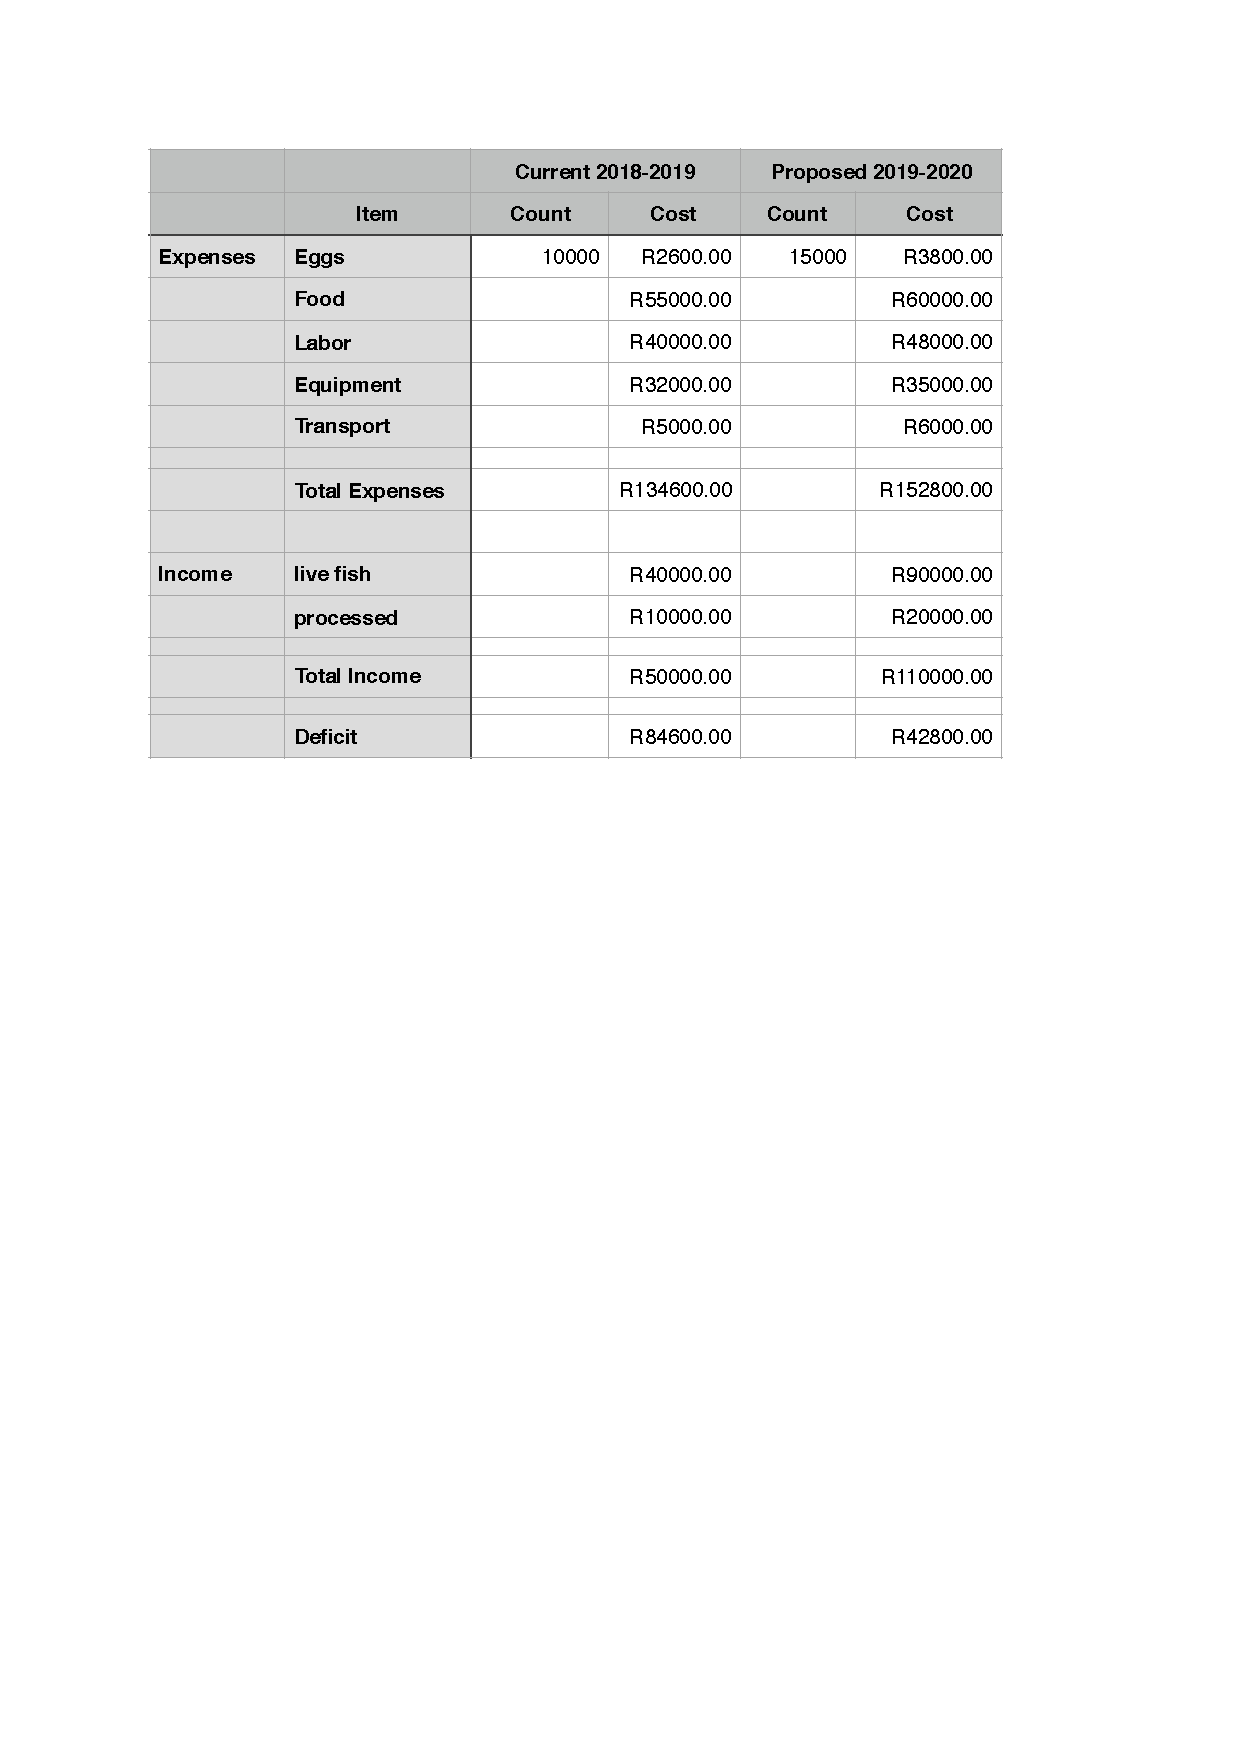
\includegraphics[scale = 0.9]{tables/TablesBudget.pdf}
   \caption{Possible Budget proposal for next season.}
  \label{tab:Budget}
\end{table}
 



\chapter{Possible Fertilisation of Mbona Trout Eggs}
 
 Currently, Mbona purchases pre-fertilised eyed eggs for their hatching trays. However it may be possible to
 strip and fertilise our own fish if we have a reasonable collection of mature female and male trout.
 These brood fish should ideally be about 3 years old. In this chapter we outline what would be required in order to accomplish this operation. These recommendations come from Gavin Chin.
 
 \section{Infrastructure}
 
 \subsection{Housing}
 Fertilised Eggs must be incubated in a "tower" that remains undisturbed in the dark for at least
 25 days. To accommodate this tower the Mbona hatcheries must purchase another shed to house the
 incubation tower. This shed can be small as only one tower is envisaged. Probably a "guard hut" residing
 on a concrete base will do.
 
\subsection{Egg towers}

The newly fertilised eggs must reside undisturbed in a {\bf tower} for about 25 days. This tower has the
following properties, see diagram in figure \ref{fig:FertilisationTower}.

\begin{figure}[H]
  \centering
   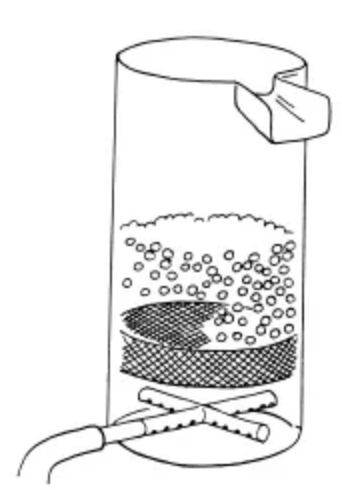
\includegraphics[scale = 0.5]{images/FertilisationTower.png}
  \caption{Fertilisation Tower.}
   \label{fig:FertilisationTower}
\end{figure}



                  \begin{itemize}
                  \item  Egg towers to stand on concrete base set through cabin floor. 
                  \item 75mm PVC tube, castellated top with light-proof lid set in 35mm thick concrete base
                  \item gravel chip diffuser, stainless steel mesh above, 
                  \item 1/2inch inlet with tee for vertical anti bubble pipe.  
                  \item Hypodermic needle set into clear plastic inlet pipe for Malachite infusion.
                  \end{itemize}
                  
 
\section{Stripping Equipment}

\begin{itemize}
\item table  
\item towel  
\item paper towel 
\item 2  large bowls  
\item 2 jars 
\item wet cloth  
\item smooth anorak 
\item one teaspoon 
\item one long feather
\item 2  large nets  
\item recovery tank with good oxygenated water
\item 2l malachite solution
\item egg tower with constant supply of oxygenated water.
\end{itemize}

\subsubsection{Malachite solution: }

                  \begin{itemize}
                  \item 2l water (preferably preboiled)
                  \item 1 x heaped teaspoon Zink free Malachite powder (Supplier details from Gavin)
                  \item Keep solution in sealed bottle.
                  \end{itemize}


\section{Workers}
\begin{itemize}
\item fish catcher 
\item runner 
\item fish stripper  
\item an assistant 
\item fish recoverer
\end{itemize}

                                       

\section{Method}

\subsection{Stripping the Hens}   

\begin{itemize}
\item Make sure both stripping bowls are completely dried using paper towel. 
Any water mixed into the eggs at this stage would result in the eggs not being fertilised.
\item Presuming the stripper is right handed, use the wet cloth to hold fish by the tail in left hand. 
\item Tuck the fish's head under your left arm hiding its eyes, (vent away from yourself).
\item Using the towel,  ask the assistant is to dry the nipple area of the fish in the direction of the tail. 
\item Strip each hen into the smaller dried bowl so that ova can be assessed.
\item Only when seen to be NOT haloed add ova to larger bowl.
\item Using the right hand the stripper milks the fish on the underbelly to expel the eggs. 
\item It may take a few strokes before the eggs appear.
\item If the belly is hard and no eggs appear, then the fish is not ready and goes in the recovery tank. 
\item If the eggs are haloed (ie translucent with an orange dot), then the eggs are too old and must not be mixed in with the other eggs. If even one egg in a batch is haloed, throw the entire batch away, but continue to strip the fish or she may become egg-bound and die. 
\item If last years eggs are expelled with good eggs, they must be removed with the teaspoon. They appear as a whitish shell.The eggs should be uniform orange in colour. 
\item Strip the fish until all eggs are out.  If the fish defecates during stripping (black  in colour), remove the faeces using the teaspoon. 
\item If the fish tenses, allow her to relax before continuing stripping. 
\item If she struggles, allow her to drop gently to the table then continue with the process.  
\end{itemize}
 
\subsection{Recovery}

\begin{itemize}
\item Take fish to recovery tank as soon as possible
\item Hold her upright under the water and closest to oxygenated water while cleaning off her body the slime
that has built up during stripping.
\item Only the slime that occured during stripping to be removed to prevent her getting a fungus.
\item Keep holding her upright until she swims away out of your hands. 
\item Do not pull her backwards through the water. 
\item The person aiding fish to recover must stand at the tank and check for fish turning on their side. 
\item The fish must be helped to remain upright to make a full recovery. 
\item Return recovered fish to their own tank within a couple of hours. 
\end{itemize}

\subsection{Stripping the Cocks}

\begin{itemize}
\item Once the females have been stripped, the catcher sends a male to be held in the same way. 
\item The milt from the male is to be stripped into one of the jars. 
\item Remove faeces if necessary. 
\item One or two males may be enough for fertilisation. 
\end{itemize}

\subsection{Fertilisation}

\begin{itemize}
\item Pour the milt into the eggs. 
\item Stir very gently with a feather until eggs are coated with milt.
\item Leave for about 10 minutes
\item Add water to the bowl until the bowl is a third to a half full. 
\item Leave for half an hour.
\item Cover to prevent light entering.
\item Flush eggs with clean water and remove dead (white) eggs.
\item Add to the tower, through which a constant supply of oxygenated water is flowing. 
\item Leave in tower overnight.
\item Next morning, pour ova into bowl with water and remove all dead eggs and replace in tower.
\item Leave for 4 days undisturbed. 
\item After 4 days treat eggs by injecting 10ml of malachite solution daily to prevent fungal infection.  
\item When eyed after about 25 days transfer to egg trays.
\end{itemize}

    


\chapter{Mbona Hatcheries Records}


\section{Record Keeping}

The various record keeping forms appear in the appendix of this document. The forms are self explanatory.
Eventually the Appendix will also contain records from years gone by if they still exist. 

\subsection{Season starting June 2018}

The 2018 season started with the arrival of $10000$ eyed Rainbow Trout eggs from the Underberg Hatchery. 
The temperature of the water at the Underberg hatchery was approximately \SI{12}{\celsius}.
The eggs arrived at Mbona at14h30 in two trays with one ice tray on the bottom and 
another ice tray on the top of the transportation cooler box.

On arrival at Mbona the temperature of the eggs in the top tray was \SI{12}{\celsius} which was brought up to
the Mbona water temp of \SI{14.6}{\celsius} by 16h00 and these eggs were then moved to bath B.

On arrival at Mbona the temp of the bottom tray was \SI{10}{\celsius} 
which was brought up to Mbona water temp of \SI{14.6}{\celsius} by 16h30 and these eggs were placed
in bath A.

Once the eggs had been transferred to the incubation baths, the process of removing dead eggs began.
In table ~\ref{tab:Incubation2018} we show how many dead eggs were removed from each bath per day
during the incubation period.

Feeding the Rainbow fry with fish food starter powder commenced on Tuesday the $12^{th}$ of June.

On Thursday the $14{th}$ of June a further $3000$ brown trout eyed eggs from the Trova Trout company 
in Sabie arrived at the Mbona Hatchery. These ova were packed in iced trays and air freighted to PmB. 
They arrived at Mbona at 9am at a temperature of \SI{5.1}{\celsius}. 
The temperature of the eggs was gradually increased to \SI{13.1}{\celsius} over a period of 5 hours. 
The ova were transferred to a hatching tray in bath C at 14h00 when the water was at 
temperature \SI{13.4}{\celsius}. 
Removal of dead ova from Bath C commenced on Friday the $15^{th}$ of June, 
see table ~\ref{tab:Incubation2018} for daily mortality counts.

\begin{table}[H]
  \centering
  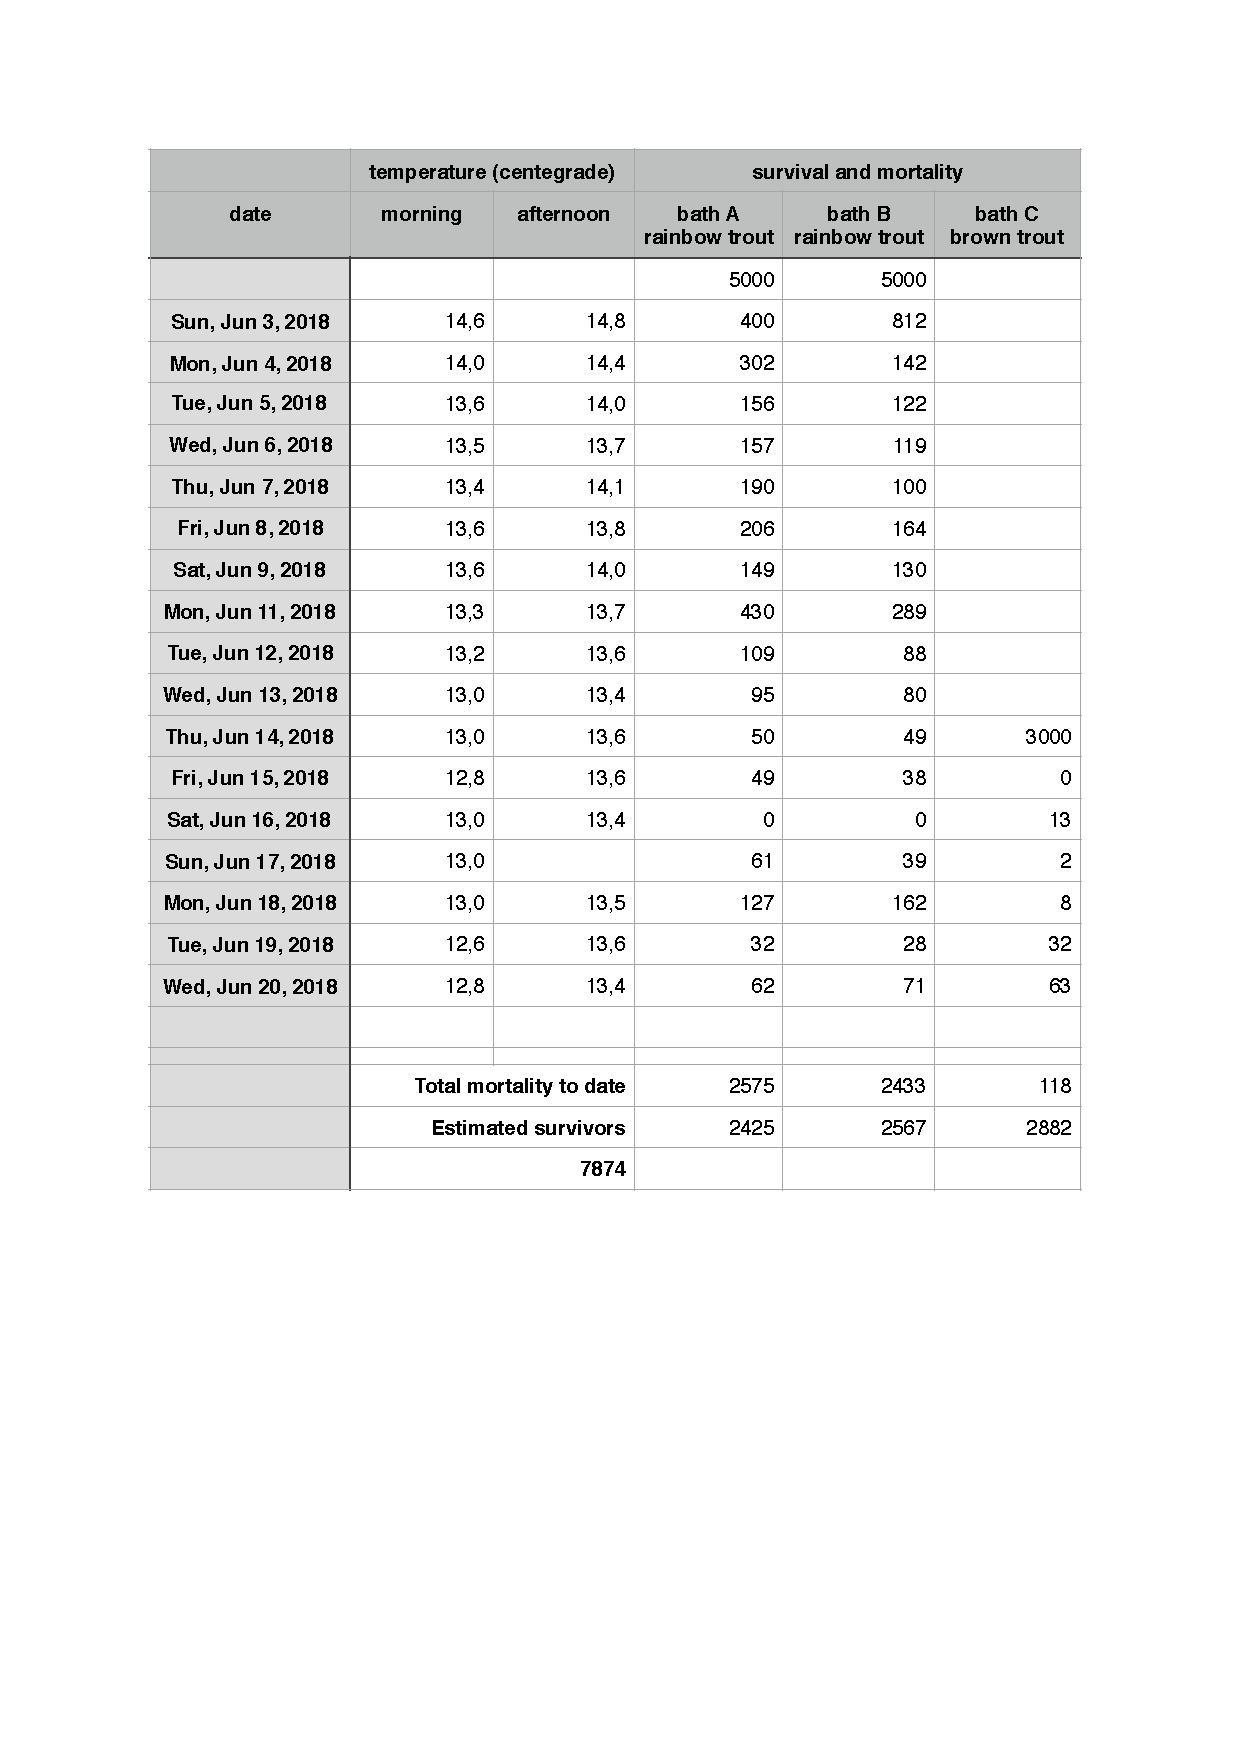
\includegraphics[scale = 0.9]{tables/TablesIncubationMortality.pdf}
   \caption{Temperature and mortality records for 2018 incubation period.}
  \label{tab:Incubation2018}
\end{table}

Assuming that the number of eggs at purchase was accurate and that dead eggs were counted accurately
table ~\ref{tab:FryRelocation2018} suggests that we could expect approximately 5000 surviving Rainbow fry 
ready for relocation to the fry tanks. So we were pleasantly surprised when the Relocation counts as 
shown in table ~\ref{tab:FryRelocation2018} indicated approximately 8000 surviving Rainbow fry.

\begin{table}[H]
  \centering
  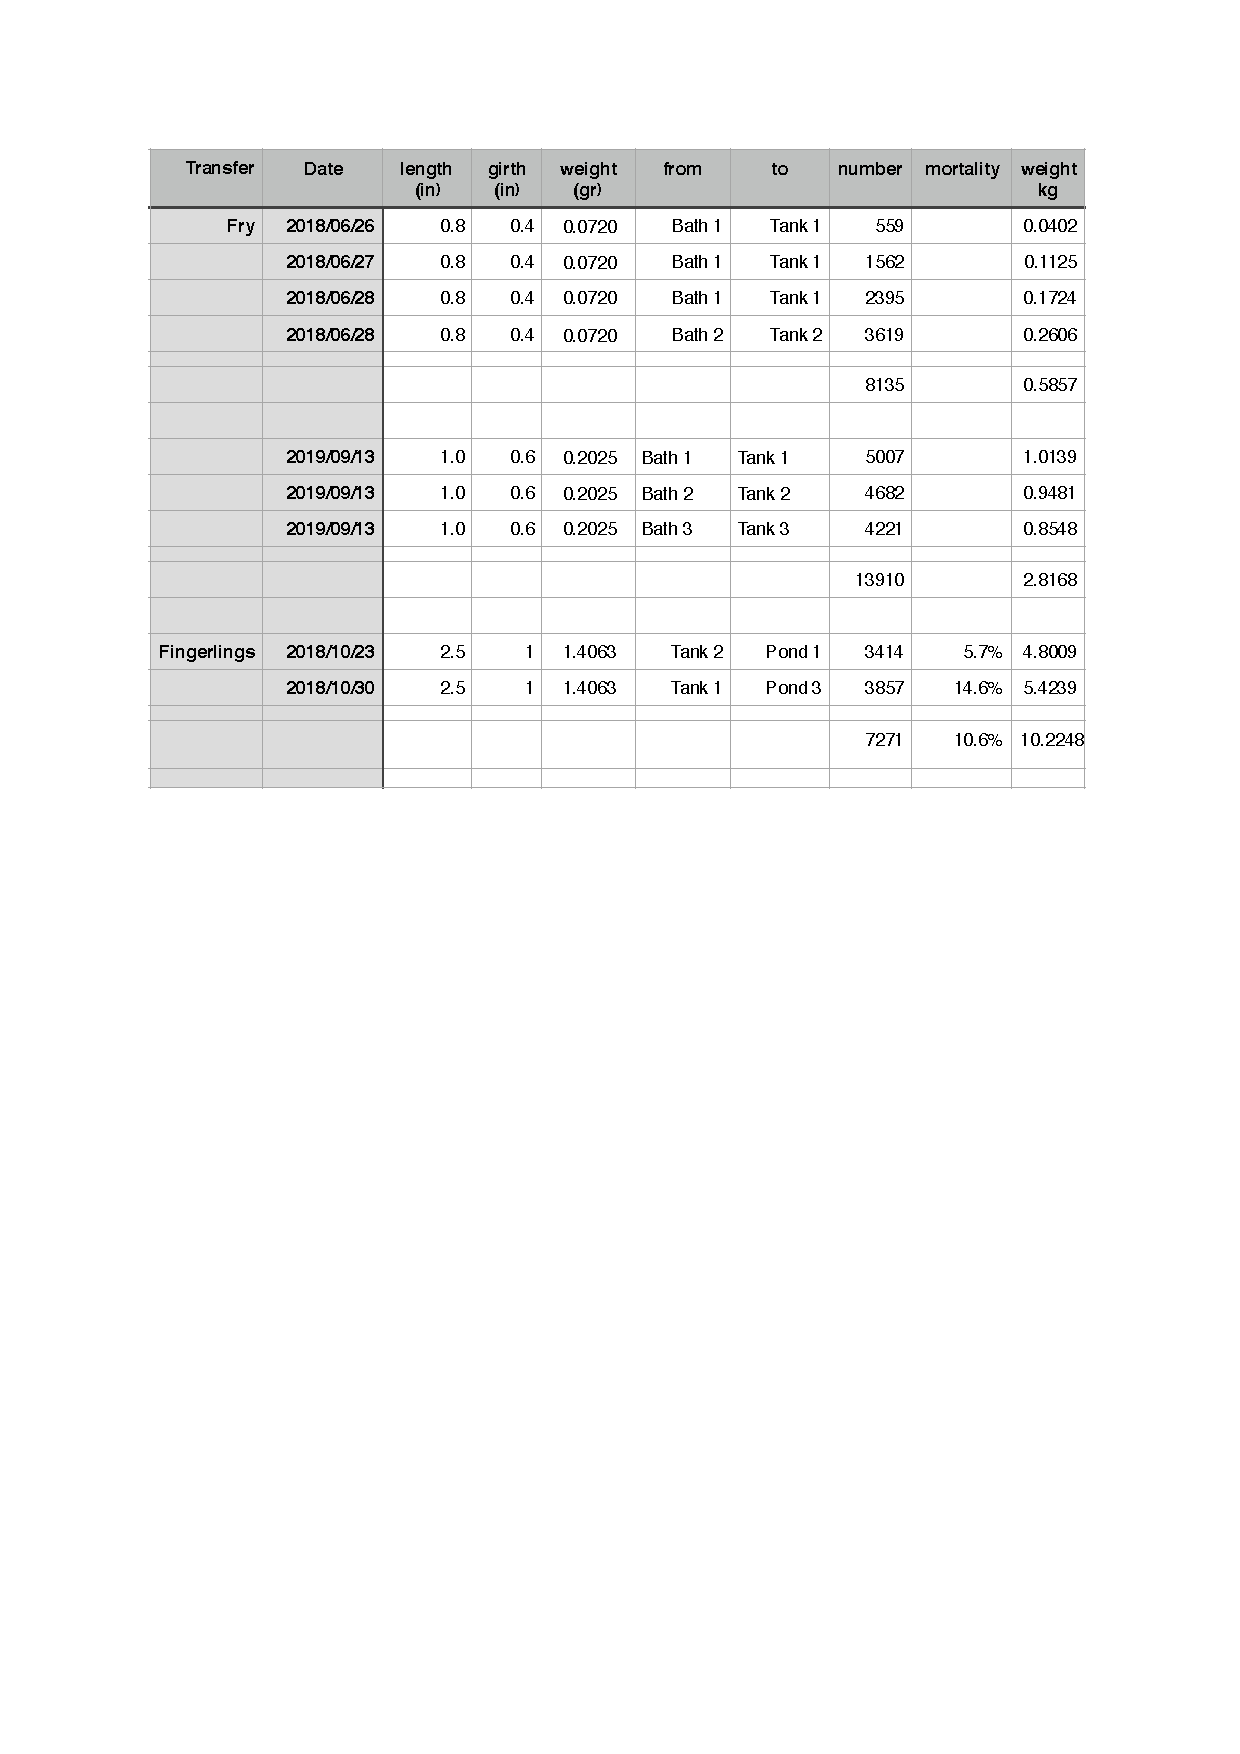
\includegraphics[scale = 0.9]{tables/TablesFryRelocationRecord.pdf}
   \caption{Counts for 2018 relocation of fry from baths to tanks.}
  \label{tab:FryRelocation2018}
\end{table}

This 40\% discrepancy is either due to receiving more eggs than expected or due to the
counting of hatched egg shells as dead eggs or to both.

\subsubsection{Rearing the fry in the tanks}
Two weeks after relocation of fry from baths to tanks we carried out length and weight measurements
on the fry. The results can be seen in table ~\ref{tab:FryGrowth} where the recommended feeding
schedule is given as computed from the suggestions given in chapter 3.

\begin{table}[H]
  \centering
  
\includegraphics[scale = 0.9]{tables/TablesFryGrowth.pdf}
   \caption{Weight and Length measurements of growing fry}
   \label{tab:FryGrowth}
\end{table}

\subsection{Sales of 2017 Trout in the 2018-2019 season}

During the 2018-19 season we sell 2017 fish live to local customers and 
when available, dressed fish to Mbona shareholders. We use the remainder
to stock our dams at Mbona. see tables, \ref{tab:ExternalSales2018}, 
 and \ref{tab:MbonaDamSales2018} below.

\begin{table}[H]
  \centering
  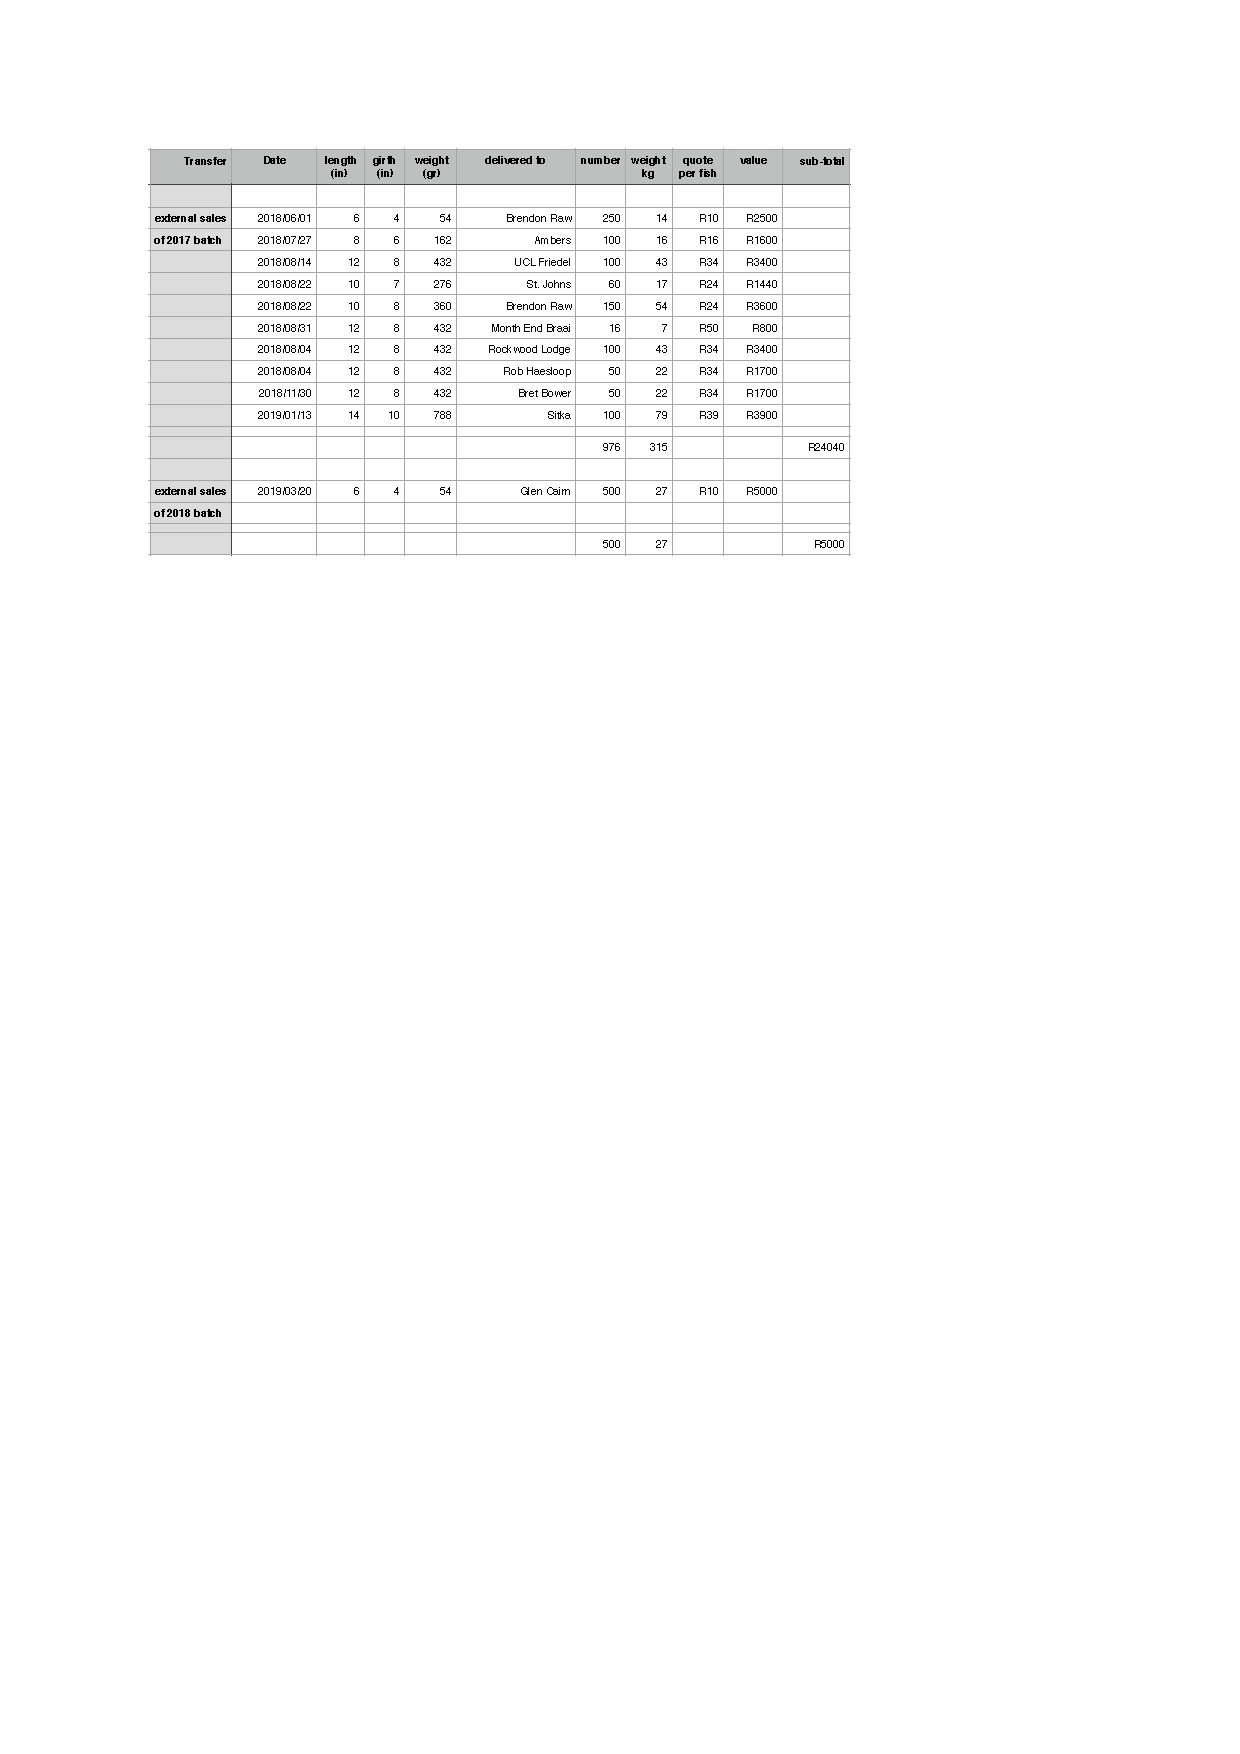
\includegraphics[scale = 1.2]{tables/TablesExternalSales.pdf}
   \caption{2018-19 sales of live fish to external customers.}
  \label{tab:ExternalSales2018}
\end{table}


\begin{table}[H]
  \centering
  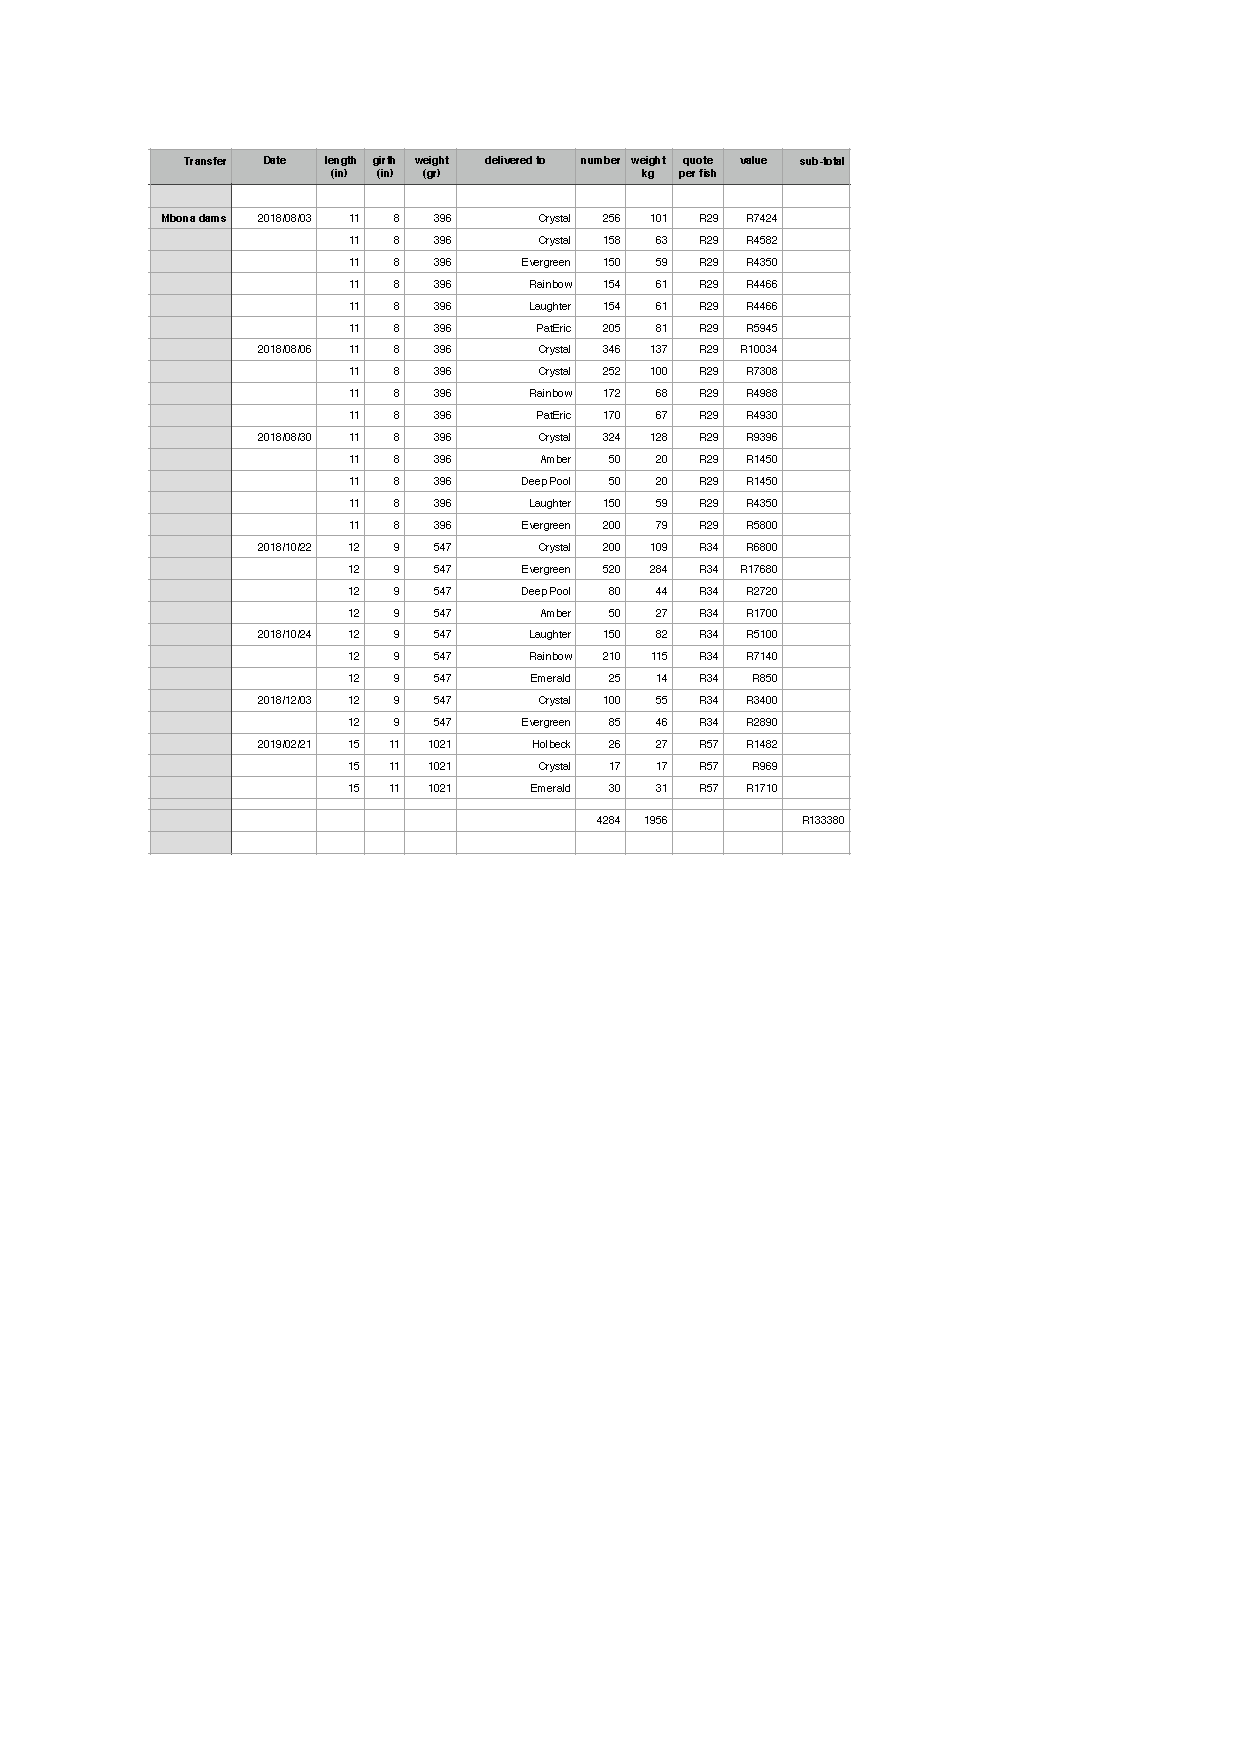
\includegraphics[scale = 1.2]{tables/TablesMbonaDamSales.pdf}
   \caption{2018-2019 stocking of Mbona dams from eggs hatched in 2017.}
  \label{tab:MbonaDamSales2018}
\end{table}

Since October 2018 we have started recouping some of our costs by selling both dressed 
and smoked trout to shareholders,
see chart \ref{fig:ShareholderSales} below.

\begin{figure}[H]
  \centering
  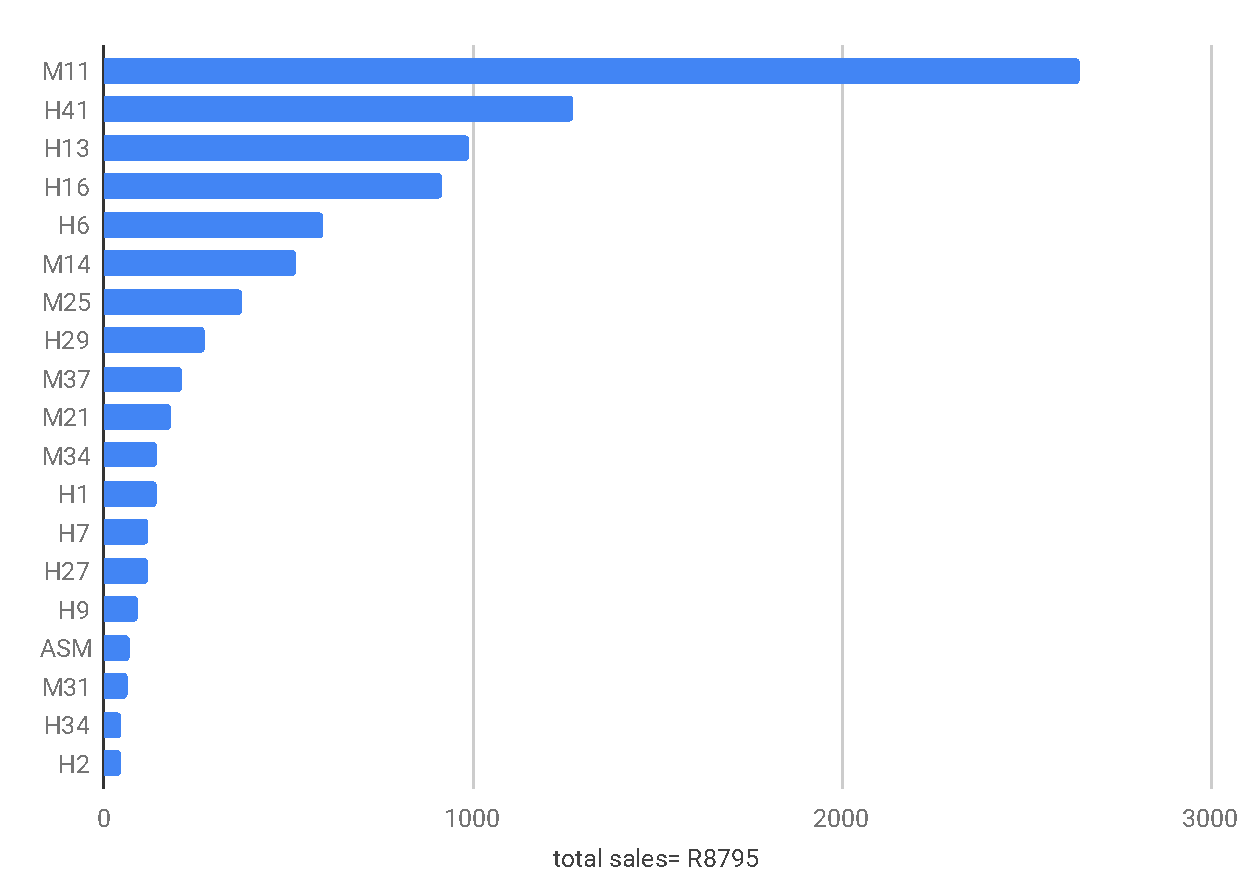
\includegraphics[scale = 0.75]{tables/MbonaTroutShareholderSales.pdf}
   \caption{Nov 2018 - May 2019 sales of dressed and smoked trout to Mbona shareholders.}
  \label{fig:ShareholderSales}
\end{figure}

\subsection{Budget proposal}

Based on the sales figures presented above and food and labour expenses made available
by the Mbona management we propose the following rudimentary budget for the 2019-2020
season. This proposal would benefit from further deliberations by the fishing committee.

\begin{table}[H]
  \centering
  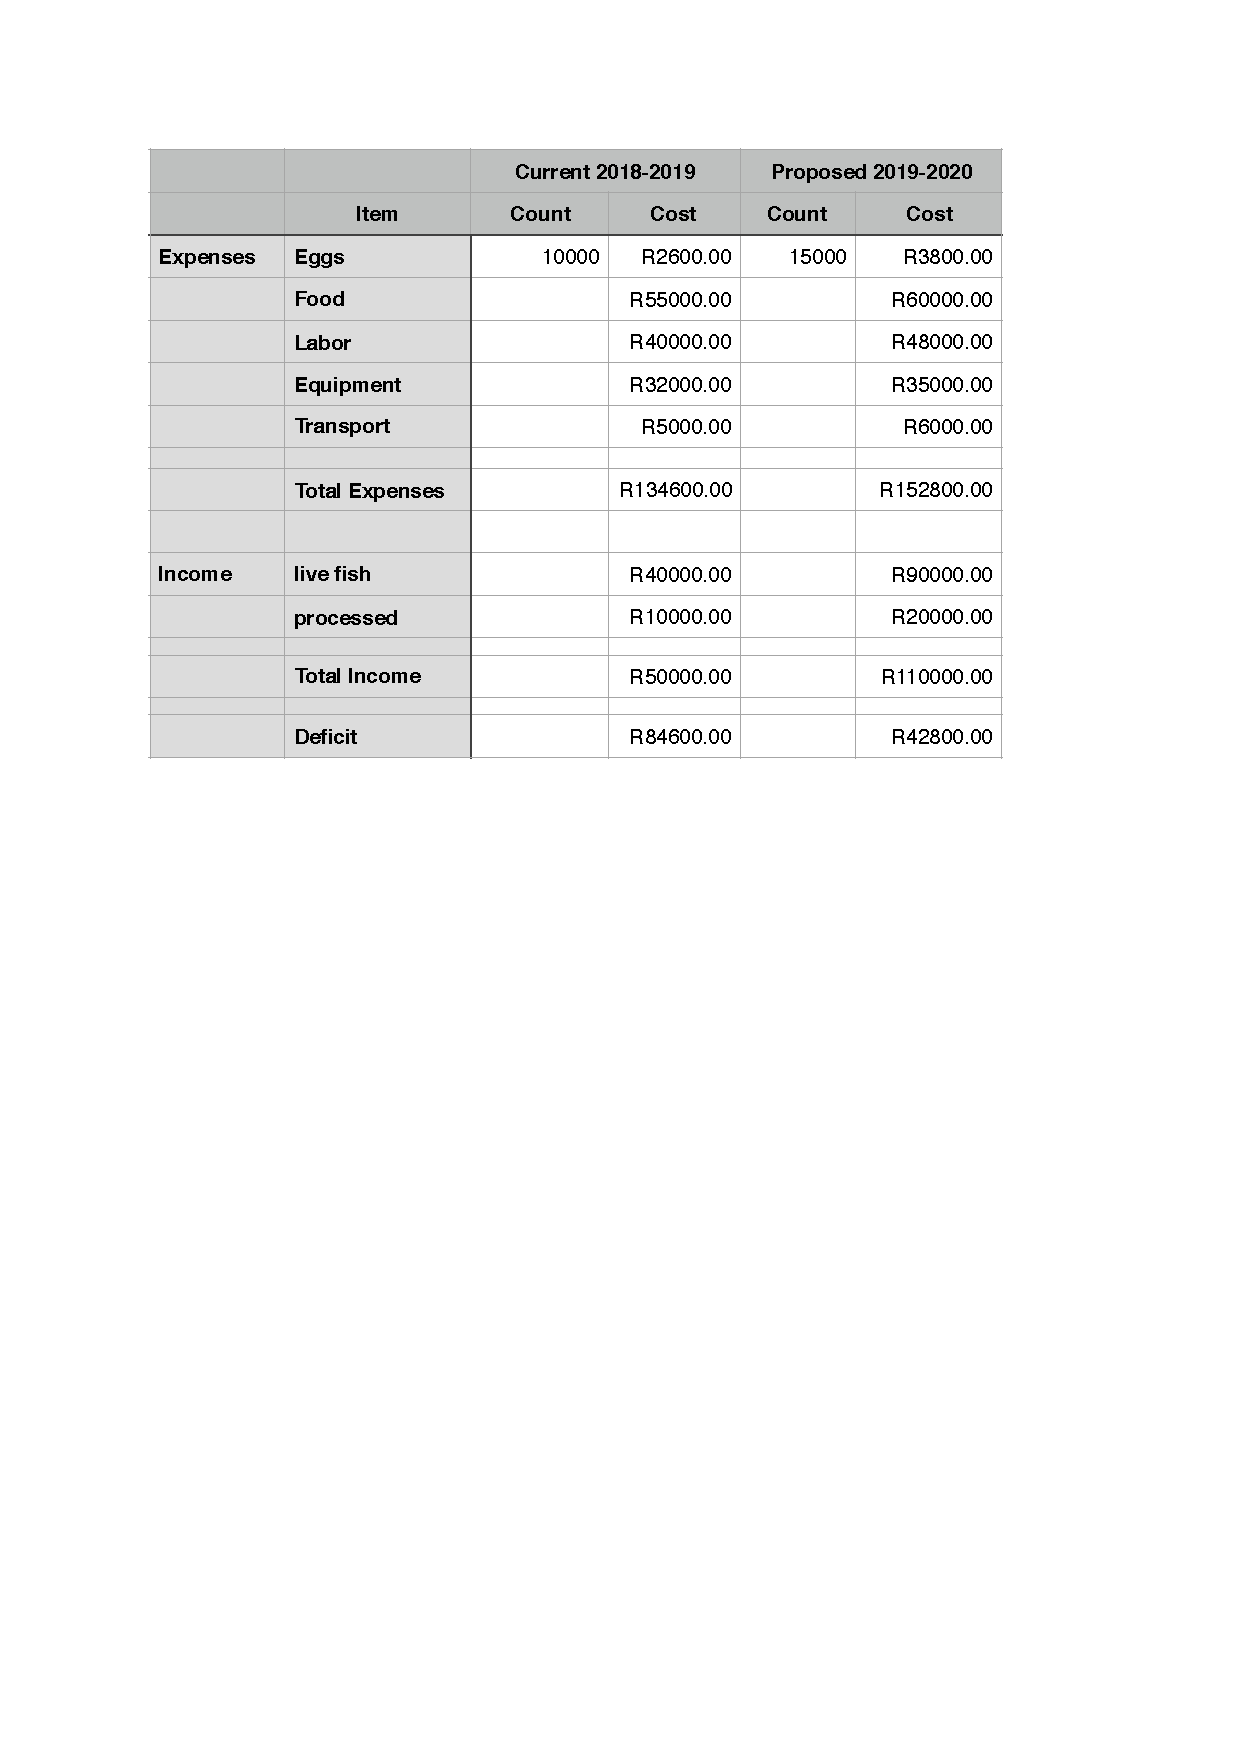
\includegraphics[scale = 0.9]{tables/TablesBudget.pdf}
   \caption{Possible Budget proposal for 2019-2020 season.}
  \label{tab:Budget}
\end{table}
 

\subsection{Fly Fishing returns}

The primary purpose for the trout rearing operation is to provide recreational
fly fishing for shareholders. It is difficult to gauge how popular fly fishing is. 

We encourage shareholders
and their guests to fill in the Mbona trout return form and tell us how many trout they have
caught and in what dam they were successful. Your returns can be submitted online
by visiting the Mbona website: 

\url{www.mbona.co.za} 

or if you are averse to using a computer you can fill in a paper based form at the Mbona gate.

In the next two charts the reader can find an analysis of trout returns since the start of
web-based record keeping.

\subsection{Mbona Trout Ladder}

\begin{figure}[H]
\centering
  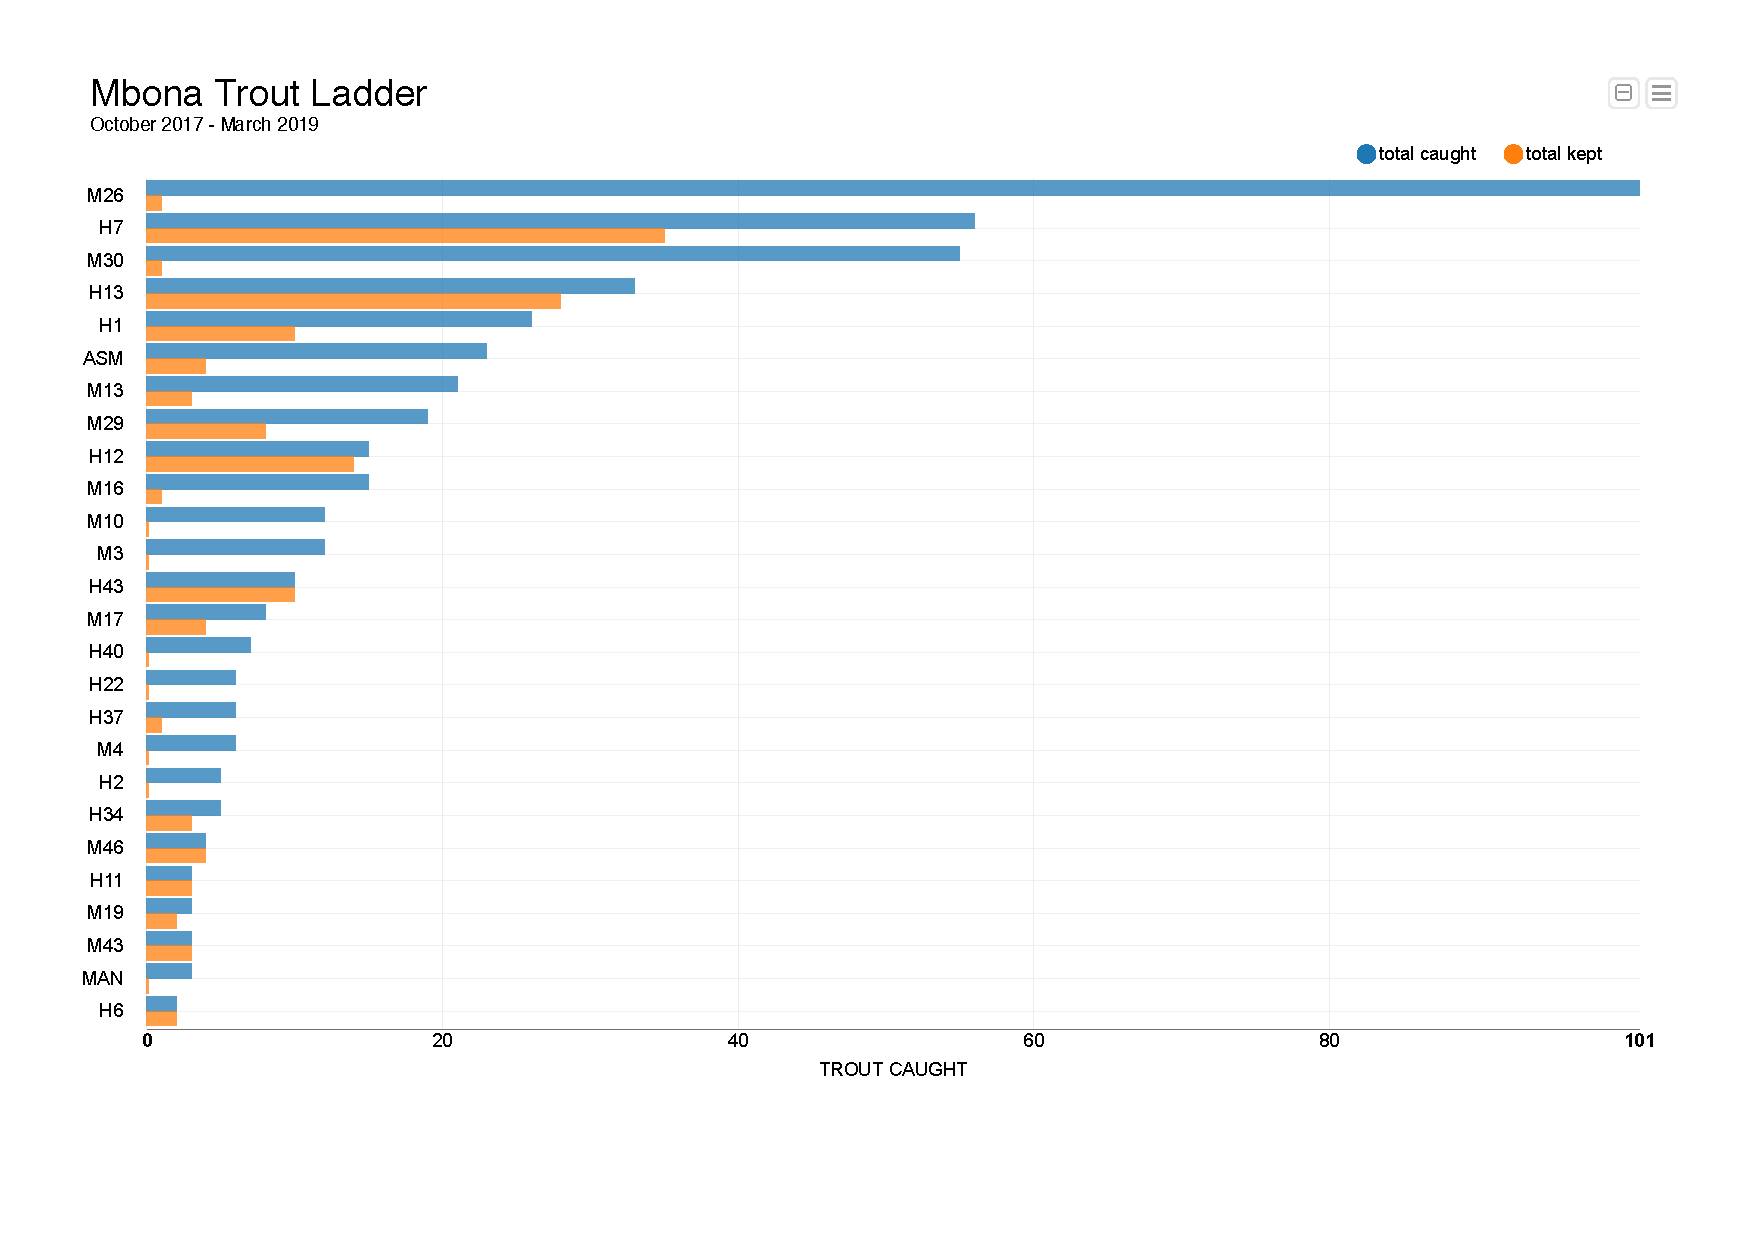
\includegraphics[scale=0.4]{tables/MbonaTroutLadder.pdf}
   \caption{Ladder showing catch and keep records for each share since web based trout returns were introduced.}
  \label{fig:MbonaTroutLadder}
\end{figure}


\subsection{Trout Catches by Dam}

\begin{figure}[H]
\centering
  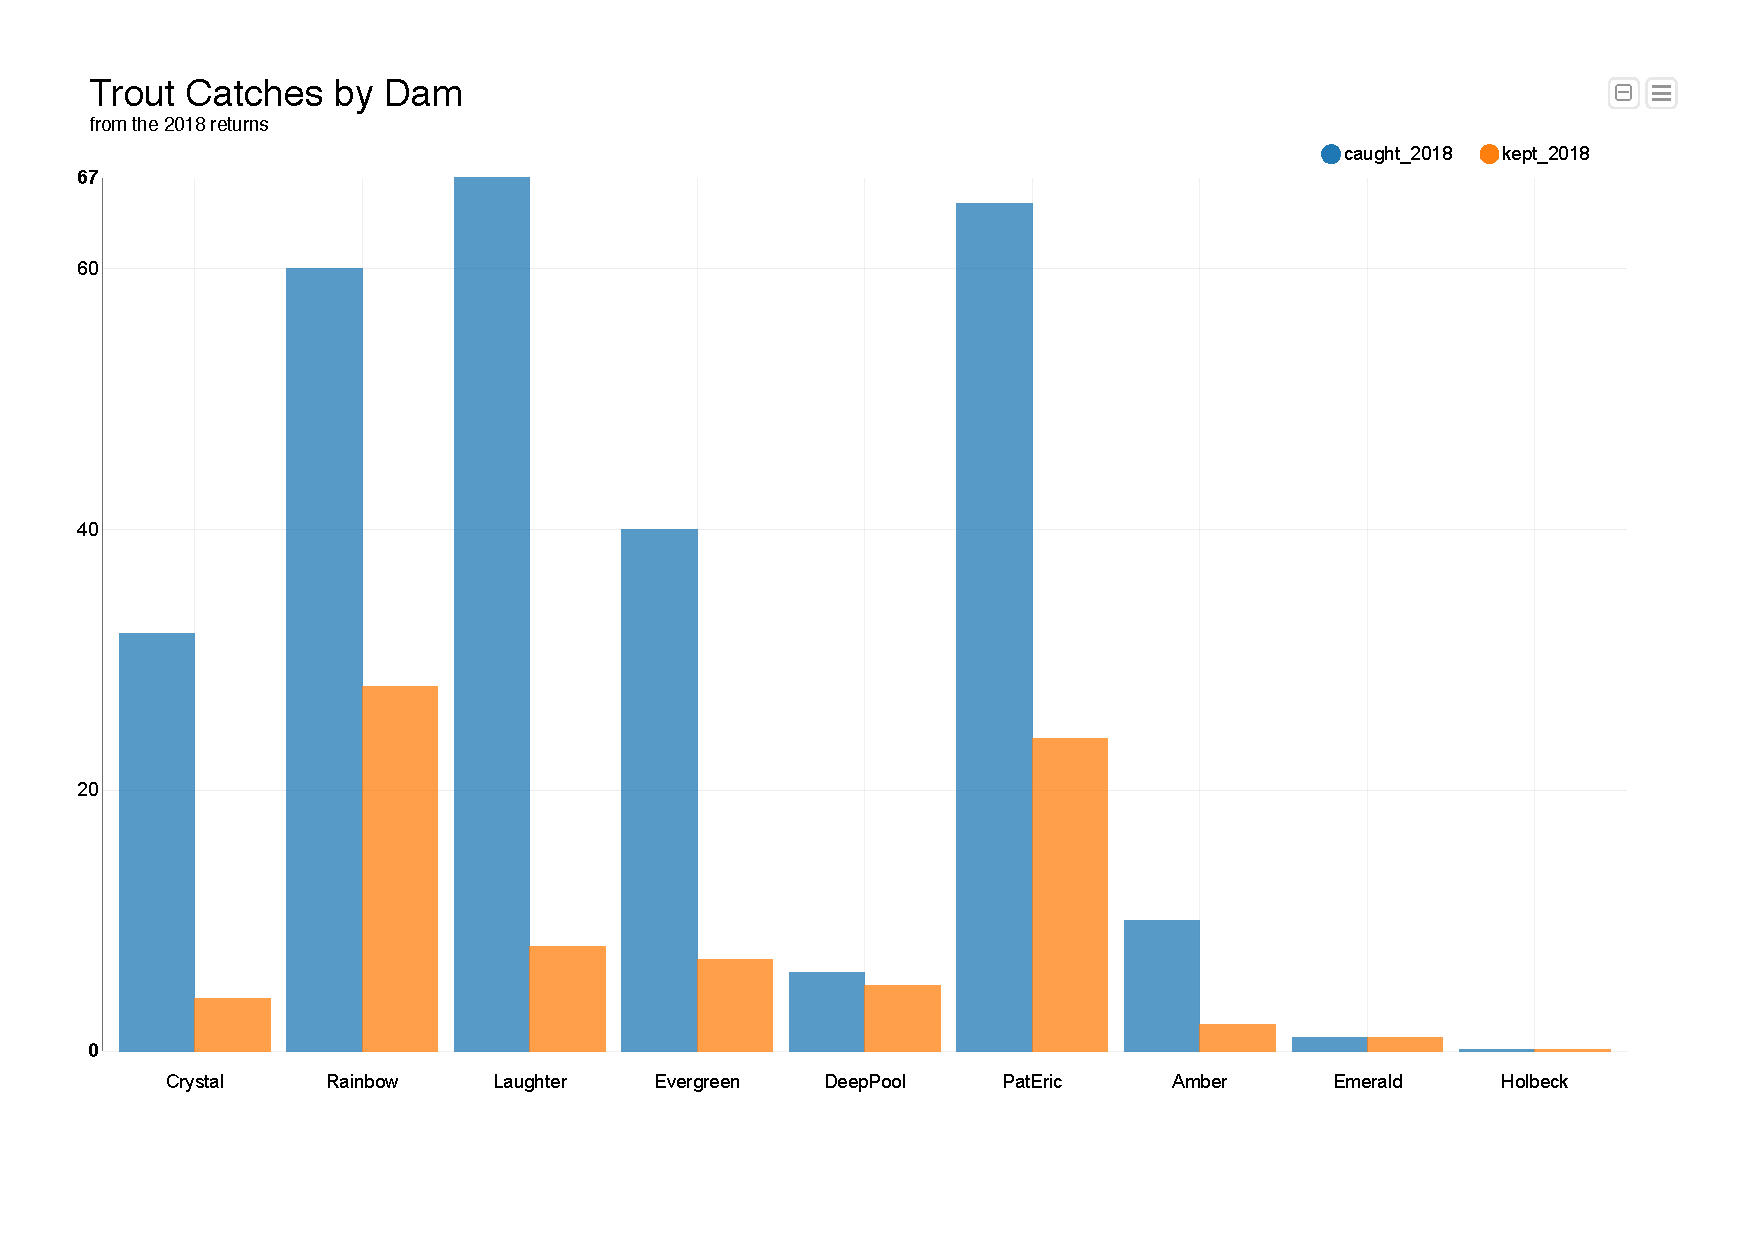
\includegraphics[scale=0.4]{tables/TroutCatchesByDam.pdf}
   \caption{Bar chart showing catch and keep records for each dam for 2018.}
  \label{fig:TroutCatchesByDam}
\end{figure}




\chapter{Trout Recipes}

In this chapter we intend to publish Trout Recipes for dishes that have been 
attempted at Mbona. Please email your trout recipes to the editor at:

\href{mailto:hugh.murrell@gmail.com}{hugh.murrell@gmail.com}

Your recipe can be in plain text with an {\bf ingrediants} section
and an {\bf instructions} section. Please attach a photo of the resulting
dish just before eating commences. See our braai trout recipe for an example.

\clearpage


\section{Robertson's Braai Trout \\ (by Hugh Murrell)}

\subsection*{ingredients}

\begin{itemize}
\item 2 Whole Trout, gilled and gutted.
\item Robertsons Spice for Fish
\item 2 lemons
\item 1 Fennel Bulb
\item 1 lemon
\item For the Yogurt Dressing:
\begin{itemize}
\item 250ml Greek Yogurt, double cream
\item 45ml mayonnaise
\item 1 lemon, juiced
\item 10ml Wholegrain Mustard
\item Robertsons Coarsely Ground Black Pepper
\end{itemize}
\end{itemize}

\subsection*{instructions}

\begin{itemize}
\item Get your fire ready to braai the fish over medium hot coals.
\item Oil the inside of your grid to ensure that the fish doesn't stick to the grid.
\item Rinse the trout well under cold water, then pat dry with a tea towel.
\item Season the fish, inside and outside, with Robertsons Spice for Fish. 
\item Use lemon and sliced fennel slices to stuff into the cuts and cavity, 
then drizzle the stuffed parts with lemon juice. 
\item Place the fish inside a large hinged grid (without any foil) 
using a few lemon slices to protect the fish, see figure \ref{fig:braaiTroutPrepared}


 
\item braai over medium hot coals on both sides for about 30 minutes in total, see figure \ref{fig:braaiTroutPrepared}.


\item For the dressing, mix all the ingredients together.
\item Transfer the fish to a large serving platter and serve with a bowl of yogurt dressing, see figure \ref{fig:braaiTroutServed}

\end{itemize}

\subsection*{results}
  
\begin{figure}[H]
\centering
  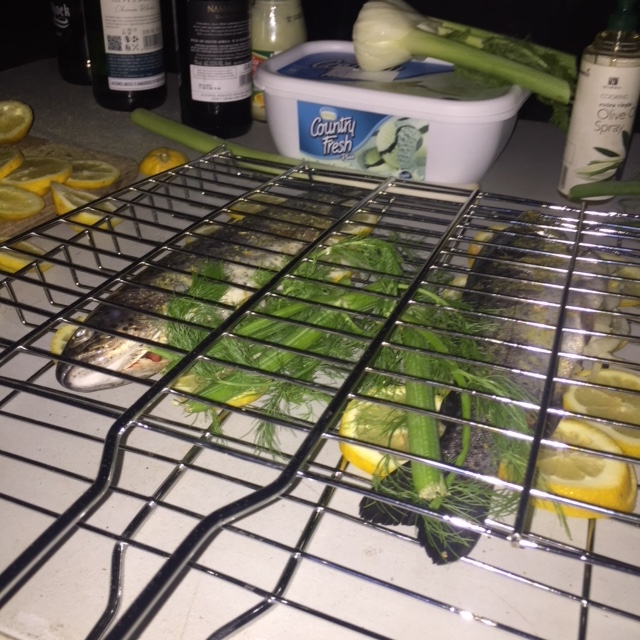
\includegraphics[scale=0.25]{recipes/braaiTroutPrepared.jpg} \hspace{1cm}  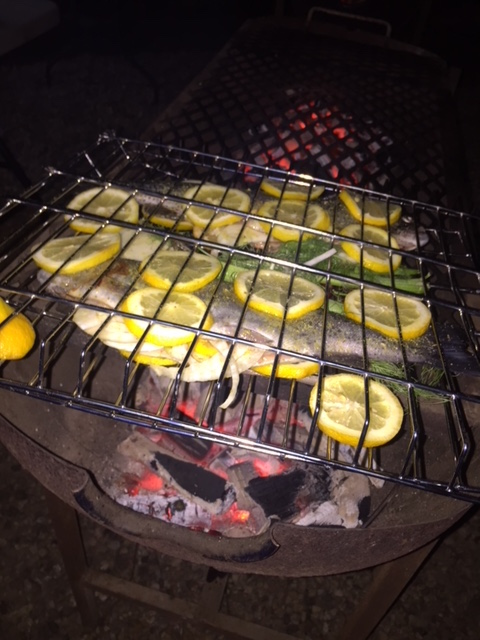
\includegraphics[scale=0.25]{recipes/braaiTroutCooking.jpg}
   \caption{Robertson's Braai Trout, prepared (left image) and on the coals (right image)}
  \label{fig:braaiTroutPrepared}
\end{figure}  


\begin{figure}[H]
\centering
  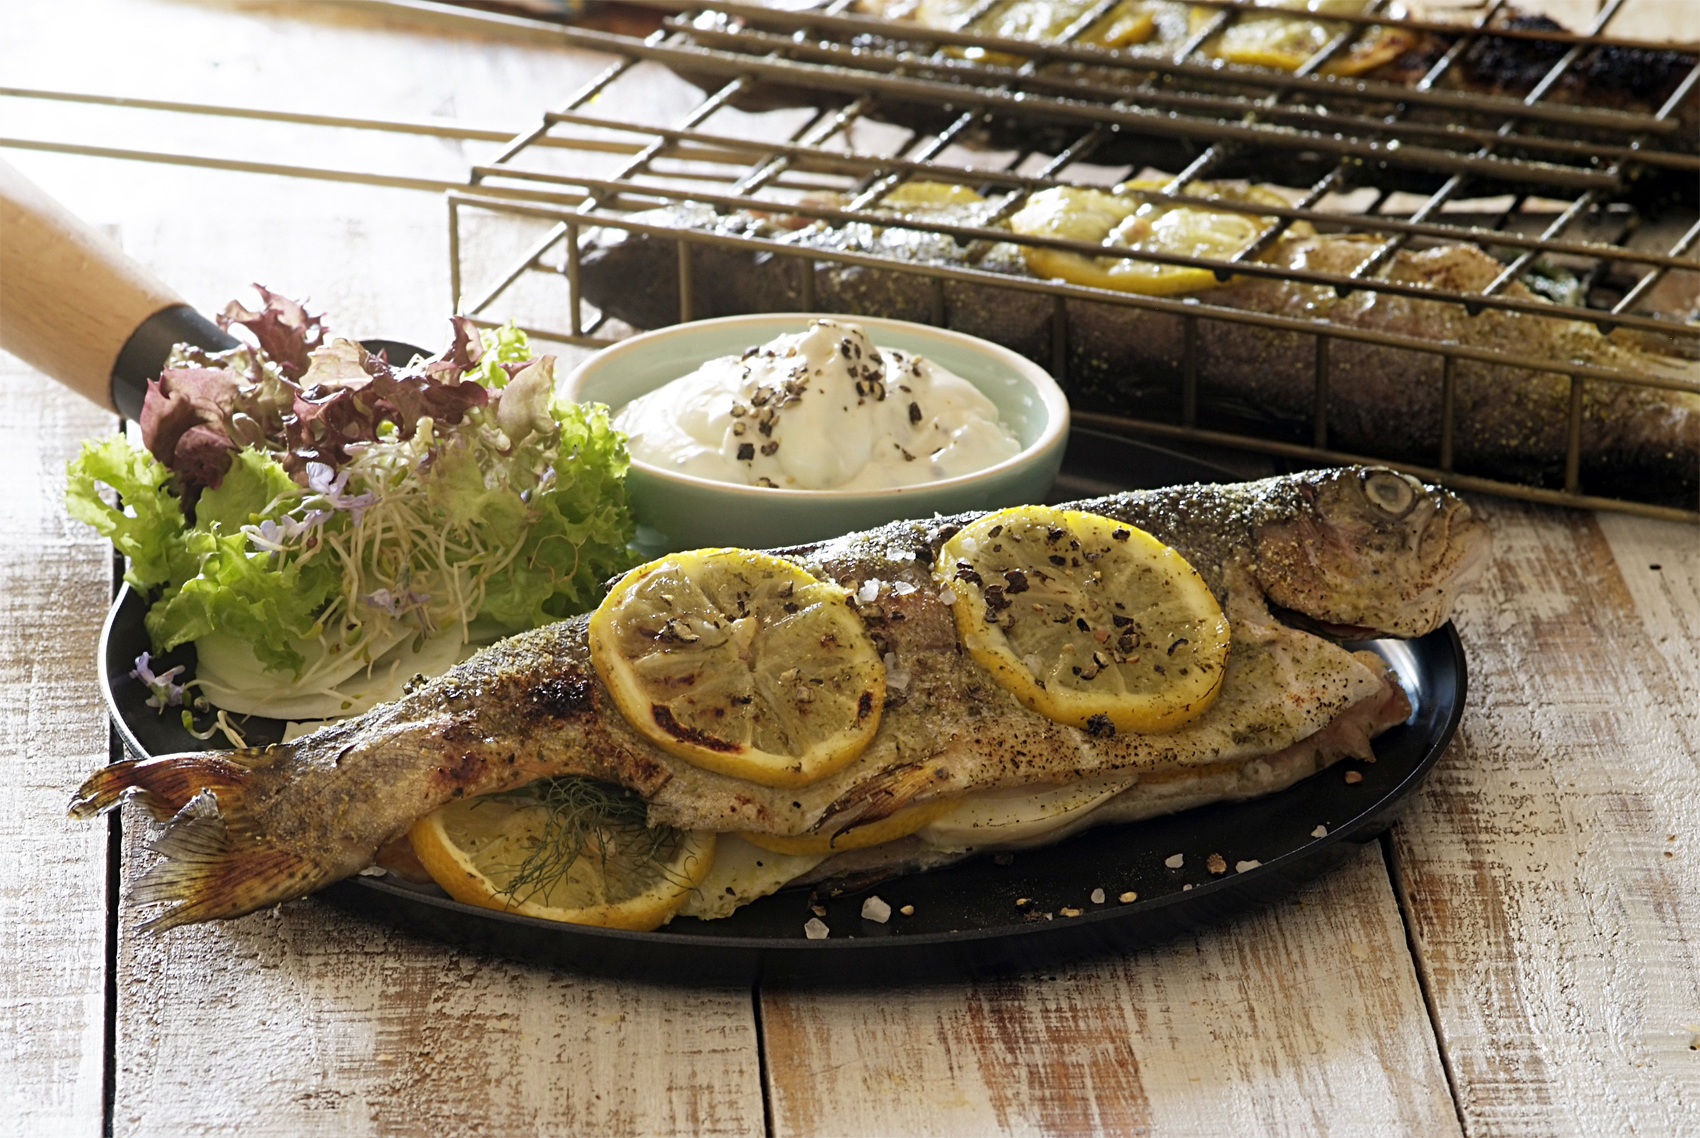
\includegraphics[scale=0.2]{recipes/braaiTroutServed.jpg}
   \caption{Robertson's Braai Trout, served and ready to be eaten.}
  \label{fig:braaiTroutServed}
\end{figure}


\section{Whole Baked Trout with Herb Salsa \\ (by Natasha Russo)} 

thanks to,  \url{http://eatdrinkpaleo.com.au/whole-baked-trout-recipe/}

\subsection*{ingredients for two trout}

\begin{itemize}
\item 2 Whole Trout, gilled, gutted and heads and tails removed.
\item For the salsa
	\begin{itemize}
		\item 1 medium red onion, peeled and roughly diced
		\item A handful of fresh basil leaves
		\item A handful of fresh parsley
		\item A few mint leaves
		\item 1 garlic clove, peeled
		\item Zest of 1 lemon
		\item Juice of half lemon 
		\item half cup olive oil
		\item 2 teaspoon sea salt
		\item half teaspoon black pepper
	\end{itemize}
\end{itemize}

\subsection*{instructions}

\begin{itemize}
	\item Preheat the oven to 200 centegrade
	\item Combine the salsa ingredients in a food processor or a blender and process into a salsa like consistency.
	\item Remove Heads and Tails and place the whole fish in a large roasting tray. 
	\item Cover the fish with the herb marinade on both sides and a little inside the fish cavity. 
	\item Bake in the oven for 20-25 minutes, on the middle shelf. 
	\item Remove and transfer to a platter or serve right in the roasting tray.
	\item Best with Spinach, Cranberry and Roast Almond Salad
\end{itemize}

\subsection*{results}
  
\begin{figure}[H]
\centering
  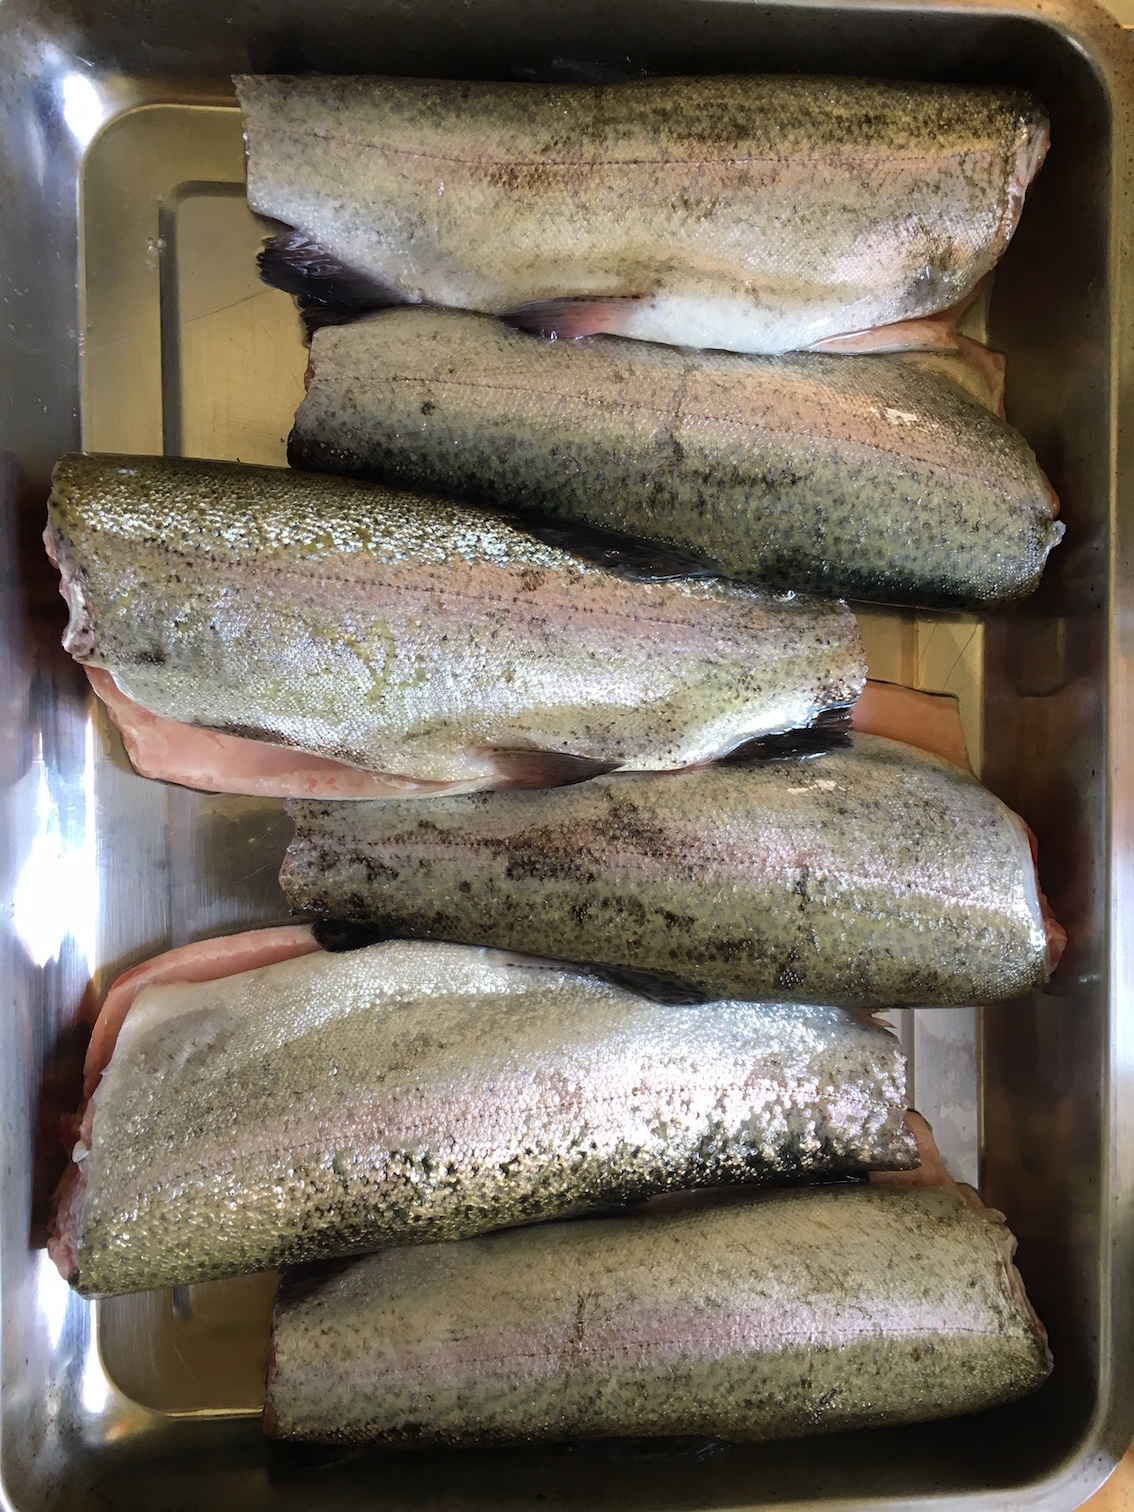
\includegraphics[scale=0.12]{recipes/NatashaPrepared.jpg} \hspace{1cm}  \includegraphics[scale=0.12]{recipes/NatashaPrecooked.jpg}
   \caption{Whole Trout, gutted (left image) and prepared (right image)}
  \label{fig:NatashaPrepared}
\end{figure}  

\begin{figure}[H]
\centering
  \includegraphics[scale=0.2]{recipes/NatashaServed.jpg}
   \caption{Natasha's Whole Baked Trout, served and ready to be eaten.}
  \label{fig:NatashaServed}
\end{figure}

\section{Mbona Cold Smoked Trout \\ (by Dave Forsyth and Guy Reen)} 

\subsection*{Ingredients}

\begin{itemize}
\item as many gutted and cleaned trout as fill fit in your smoker.
\item healthy supply of coarse salt
\item very sharp filleting knife
\item pin bone tweezers
\item indoor hanging space
\item cold smoking kiln
\item wood chips
\item vacuum packer
\end{itemize}

\subsection*{instructions}

\begin{itemize}
	\item Fillet the trout, fig \ref{fig:SmokingProceedure}A
	\item Dry and salt fillets librally.
	\item after 2 hours, wash salt off fillets and dry.
	\item hang fillets indoors overnight with fan running, fig \ref{fig:SmokingProceedure}B
	\item light wood chips and allow smoke to enter chamber from a distance, fig \ref{fig:SmokingProceedure}C
	\item place fillets in smoking chamber, fig \ref{fig:SmokingProceedure}D
	\item smoke for 2.5 hours (as long as wood chips last)
	\item remove pin bones, fig \ref{fig:SmokingProceedure}E
	\item vacuum pack fillets, fig \ref{fig:SmokingProceedure}F
\end{itemize}

\subsection*{results}
  
\begin{figure}[H]
\centering
\includegraphics[height=120pt]{recipes/smoking/RainbowFillets.jpg} \includegraphics[height=120pt]{recipes/smoking/SaltedFillets.jpg} \\
\includegraphics[height=140pt]{recipes/smoking/SmokingApparatus.jpg} \includegraphics[height=140pt]{recipes/smoking/FilletChamber.jpg} 
\includegraphics[height=140pt]{recipes/smoking/RemovingPinBones.jpg} \\
\includegraphics[height=180pt]{recipes/smoking/VacumePacked.jpg} 
   \caption{Smoking proceedure: A: Rainbow fillets, B: salted trout fillets hanging, C: apparatus with burning wood chips some distance from smoking chamber, D: fillets in smoking chamber, E: removing the pin bones, F: vacuum packed and ready for sale}
  \label{fig:SmokingProceedure}
\end{figure}  

\section{Smoked Trout with Cucumber Mousse \\ (by Dave Forsyth)}

\subsection*{ingredients}

\begin{itemize}
\item 1 Mbona smoked trout fillet
\item 1 packet of savoury biscuits
\item and for the mousse
\begin{itemize}
\item 1 greengage jelly (or 1 envelope gelatin)
\item 1 peeled and grated cucumber 
\item mayonaise and full cream
\item white vinegar, chopped mint, grated onion, horse-radish source
\end{itemize}
\end{itemize}

\subsection*{instructions}

\begin{itemize}
\item slice byte size medallions from Trout fillet.
\item for the mousse
\begin{itemize}
\item add jelly to 284 ml boiling water
\item add 2T white vinigar and allow to start setting
\item add whole grated cucumber 
\item add 1T chopped mint, 1T grated onion and 1t horse-radish source.
\item add 1c mayonaise/cream mixture
\item place in fish mould and refrigerate
\end{itemize}
\item arrange trout medallions and biscuits on one plate and upend cucumber mousse on another plate and serve as shown in figure \ref{fig:daveStarter}
\end{itemize}

\subsection*{results}
  
\begin{figure}[H]
\centering
  \includegraphics[scale=0.1]{recipes/DaveSmokedTroutWithCucumberMousse.jpg} 
     \caption{Dave's Smoked Trout with Cucumber Mousse starter}
  \label{fig:daveStarter}
\end{figure}  


\begin{appendices}

\chapter{Tables}

\section{Contact Details}

\subsection{Local Mbona Knowledge}

\begin{table}[H]
  \centering
  \begin{tabular}{|c|c|c|}
    \hline
       Person & Position & email  \\ \hline
       Dave Forsyth & manager & \href{mailto:manager.mbona@iuncapped.co.za}{\nolinkurl{manager.mbona@iuncapped.co.za}} \\ \hline
       Guy Reen & assist manager & \href{mailto:assist.mbona@iuncapped.co.za}{\nolinkurl{assist.mbona@iuncapped.co.za}} \\ \hline
       Dennis Dyer & trout chairman & \href{mailto: dennisd@surfafrica.net}{\nolinkurl{ dennisd@surfafrica.net}} \\ \hline 
       Pierre Olivier & shareholder & \href{mailto:pierre@pierrecraft.co.za}{\nolinkurl{pierre@pierrecraft.co.za}} \\ \hline
       Bernard McDonald & shareholder & \href{mailto:jmcdonaldh7@gmail.com}{\nolinkurl{jmcdonaldh7@gmail.com}} \\ \hline
       Hugh Murrell & shareholder & \href{mailto:hugh.murrell@gmail.com}{\nolinkurl{hugh.murrell@gmail.com}} \\ \hline
       Ronnie Ritchie & shareholder & \href{mailto:karklooflady@iuncapped.co.za}{\nolinkurl{karklooflady@iuncapped.co.za}} \\ \hline
       Justin Pinington & shareholder & \href{mailto: justingwc@gmail.com}{\nolinkurl{ justingwc@gmail.com}} \\ \hline      
       Gareth Powell & consultant & \href{mailto:gpsafari@gmail.com}{\nolinkurl{gpsafari@gmail.com}} \\ \hline
     \end{tabular} 
     \caption{Local Knowledge, Contact Details}
  \label{tab:LocalKnowledgeContactDetails}
\end{table}

\subsection{Suppliers}

\begin{table}[H]
  \centering
  \begin{tabular}{|c|c|c|c|}
    \thickhline
    {\bf Item} & {\bf Contact} & {\bf Company / district / email} & {\bf phone}  \\ \thickhline
    trout eggs & Wolf Auni & Giant's Cup Hatchery & Underberg \\
              &  & Underberg & 033 7011511 \\
              &  & \href{mailto:troutcup@vodamail.co.za}{\nolinkurl{troutcup@vodamail.co.za}} 
              &    \\ \hline
              & Renier & Lunsklip & 013 2351287 \\
              & &  Lydenberg  & 082 4546017  \\ \hline
              & Simon Bunn & Peak Trout &  083 3755571 \\
              & & Cathedral Peak Hotel  & \\ \hline
   trout food &  Ntoko or Phumi      &  AVI feeds, Pinetown &  0317660016    \\
              &  &   with deliveries to Hopewell  &  \\ \hline
   grass carp & Francious Classen & De Rust Hatchery & 023 6162444 \\
                    & & Swllendam & \\
                    & &  \href{mailto:info@outdoorarena.co.za}{\nolinkurl{info@outdoorarena.co.za}} 
                    &  \\ 
                    & & R150 - R300 per fish &  \\ \hline
    chubby head  & Rudolf duToit & private farm & 083 2784848 \\
    barbs   & &  Karkloof &  \\ \hline
    chemicals &  &  &  \\
              &   &   & \\ \hline
              \thickhline
  \end{tabular} 
   \caption{Suppliers of trout eggs, trout feed, chemicals and other fish}
 
  \label{tab:SupplierContactDetails}
\end{table}

\subsection{Customers}

\begin{table}[H]
  \centering
 \begin{tabular}{|c|c|c|c|}
 \thickhline
   {\bf contact} & {\bf district} & {\bf phone} & {\bf email}  \\ \thickhline
    Brendan Raw & Jettison Timbers & 083 6832039  & bblraw@mweb.co.za \\ \hline 
     Douglas Benson & Glenrock Estate & 087 8085757 & douglas@glenrock.co.za \\ \hline
     Neville & Siteka Estate & 083 4522241 & \\ \hline
    Alan Bailey & Amber Valley & & em@ambervalleybc.co.za\\ \hline
    Mr. Farhaad & Rainbow Retreat & 082 5510247 & \\ \hline
    Friedel Eggers & UCL &  & eggers@ucl.co.za \\ \hline
    Wendy Curle & Rietvlie &  & wendycurle@vodamail.co.za\\ \hline
    Rex Fey & Kokstad &  & \\ \hline
     Whispering Water & Dargle &  & \\ \hline
     Sunset Farm & Mooiriver & 079 6244030 & fam@mweb.co.za \\ \hline
     Justin Pinington & fishing club & & \\ \hline
      Nick Nolden & Nyamvubu & & nick@noldenbros.co.za \\ \hline
     Judy Cole & Siteka & 083 4522241 & rbdservices1@gmail.com \\ \hline
     Juanita & Kambrook Farm & & Juanita@iconstruction.co.za \\ \hline
     Gareth Powell & Glen Cairn & & \href{mailto:gpsafari@gmail.com}{\nolinkurl{gpsafari@gmail.com}} \\ \hline
                   \thickhline
  \end{tabular} 
  \caption{Potential customers for live trout}
  \label{tab:CustomerContactDetails}
\end{table}

\subsection{Terms and Conditions}

\begin{itemize}
\item On enquiry the customer is provided with a quote for $N$ fish at an
average size of $X$ inches to be delivered on date $D$ to the customer
specified dam at $R$ rands per kilometre return trip. See table \ref{tab:TablesFishPrices}
for the current fish price and table \ref{tab:TransportationNumbers} for
the number of fish that can be transported in one trip.
\item If the customer accepts the quote then he or she must pay in full
before the quote expires and before delivery takes place.
\item The customer must be present and count the fish when the delivery is made
\item A photograph of the customer at the delivery site
on the day of delivery must be recorded and kept.
\end{itemize}

\newpage

\section{Record Forms:}

\clearpage\pagestyle{empty}
\begin{landscape}

\subsection{Mbona Hatchery Counting Aid}


\begin{tabular}{|c|c|c|c|c|}
\hline
Date: \hspace{3cm} & From: \hspace{3cm} & To: \hspace{3cm} & Size (inch)\hspace{1cm}  & Count \hspace{1cm} \\  \hline
                               &                                  &                              &                                         & \\ 
                               &                                  &                              &                                         & \\ 
                               &                                  &                              &                                         & \\ \hline
\end{tabular}

\vspace{1cm}

 \begin{tabular}{ccccccccccc}
 \hline
    5 & 10 & 15 & 20 & 25 & 30 & 35 & 40 & 45 & 50 & total \\ \hline
    / / / / / & / / / / / & / / / / / & / / / / / & / / / / / & / / / / / & / / / / / & / / / / / & / / / / / & / / / / /  & 50 \\
     / / / / / & / / / / / & / / / / / & / / / / / & / / / / / & / / / / / & / / / / / & / / / / / & / / / / / & / / / / /  & 100 \\
      / / / / / & / / / / / & / / / / / & / / / / / & / / / / / & / / / / / & / / / / / & / / / / / & / / / / / & / / / / / & 150 \\
       / / / / / & / / / / / & / / / / / & / / / / / & / / / / / & / / / / / & / / / / / & / / / / / & / / / / / & / / / / /  & 200\\
        / / / / / & / / / / / & / / / / / & / / / / / & / / / / / & / / / / / & / / / / / & / / / / / & / / / / / & / / / / /  & 250 \\
         / / / / / & / / / / / & / / / / / & / / / / / & / / / / / & / / / / / & / / / / / & / / / / / & / / / / / & / / / / /  & 300 \\
     / / / / / & / / / / / & / / / / / & / / / / / & / / / / / & / / / / / & / / / / / & / / / / / & / / / / / & / / / / / & 350 \\
      / / / / / & / / / / / & / / / / / & / / / / / & / / / / / & / / / / / & / / / / / & / / / / / & / / / / / & / / / / /  & 400 \\
       / / / / / & / / / / / & / / / / / & / / / / / & / / / / / & / / / / / & / / / / / & / / / / / & / / / / / & / / / / / & 450 \\
        / / / / / & / / / / / & / / / / / & / / / / / & / / / / / & / / / / / & / / / / / & / / / / / & / / / / / & / / / / / & 500 \\ \
         / / / / / & / / / / / & / / / / / & / / / / / & / / / / / & / / / / / & / / / / / & / / / / / & / / / / / & / / / / /  & 550 \\
     / / / / / & / / / / / & / / / / / & / / / / / & / / / / / & / / / / / & / / / / / & / / / / / & / / / / / & / / / / /  & 600 \\
      / / / / / & / / / / / & / / / / / & / / / / / & / / / / / & / / / / / & / / / / / & / / / / / & / / / / / & / / / / / & 650 \\
       / / / / / & / / / / / & / / / / / & / / / / / & / / / / / & / / / / / & / / / / / & / / / / / & / / / / / & / / / / /  & 700\\
        / / / / / & / / / / / & / / / / / & / / / / / & / / / / / & / / / / / & / / / / / & / / / / / & / / / / / & / / / / /  & 750 \\
         / / / / / & / / / / / & / / / / / & / / / / / & / / / / / & / / / / / & / / / / / & / / / / / & / / / / / & / / / / /  & 800 \\
     / / / / / & / / / / / & / / / / / & / / / / / & / / / / / & / / / / / & / / / / / & / / / / / & / / / / / & / / / / / & 850 \\
      / / / / / & / / / / / & / / / / / & / / / / / & / / / / / & / / / / / & / / / / / & / / / / / & / / / / / & / / / / /  & 900 \\
       / / / / / & / / / / / & / / / / / & / / / / / & / / / / / & / / / / / & / / / / / & / / / / / & / / / / / & / / / / / & 950 \\
        / / / / / & / / / / / & / / / / / & / / / / / & / / / / / & / / / / / & / / / / / & / / / / / & / / / / / & / / / / / & 1000 \\ \hline
  \end{tabular} 

\clearpage 
\end{landscape}

\subsection{Mbona Hatchery Trout Relocation Record}
\renewcommand{\arraystretch}{2.0}
\vspace{1cm}
 \begin{tabular}{|c|c|c|c|c|}
 \hline
    Date \hspace{2cm} & Quantity & Size (inches)  & From \hspace{2.5cm} & To \hspace{2.5cm} \\ \hline
             &               &          &          &      \\ \hline
             &               &          &          &      \\ \hline
           &               &          &          &      \\ \hline
           &               &          &          &      \\ \hline
           &               &          &          &      \\ \hline
           &               &          &          &      \\ \hline
           &               &          &          &      \\ \hline
           &               &          &          &      \\ \hline
           &               &          &          &      \\ \hline
           &               &          &          &      \\ \hline
           &               &          &          &      \\ \hline
           &               &          &          &      \\ \hline
           &               &          &          &      \\ \hline
           &               &          &          &      \\ \hline
           &               &          &          &      \\ \hline
  \end{tabular} 
 

\pagestyle{plain}
\newpage

\subsection{Trout Return Form}

\begin{figure}[H]
\centering
  \includegraphics[scale=1]{tables/TablesTroutReturns.pdf}
   \caption{Return Form to be filled in by visitors on departure at the main gate.}
  \label{fig:TroutReturnForm}
\end{figure}




\end{appendices}

%\chapter{Mbona Hatcheries Records}


\section{Record Keeping}

The various record keeping forms appear in the appendix of this document. The forms are self explanatory.
Eventually the Appendix will also contain records from years gone by if they still exist. 

\subsection{Season starting June 2018}

The 2018 season started with the arrival of $10000$ eyed Rainbow Trout eggs from the Underberg Hatchery. 
The temperature of the water at the Underberg hatchery was approximately \SI{12}{\celsius}.
The eggs arrived at Mbona at14h30 in two trays with one ice tray on the bottom and 
another ice tray on the top of the transportation cooler box.

On arrival at Mbona the temperature of the eggs in the top tray was \SI{12}{\celsius} which was brought up to
the Mbona water temp of \SI{14.6}{\celsius} by 16h00 and these eggs were then moved to bath B.

On arrival at Mbona the temp of the bottom tray was \SI{10}{\celsius} 
which was brought up to Mbona water temp of \SI{14.6}{\celsius} by 16h30 and these eggs were placed
in bath A.

Once the eggs had been transferred to the incubation baths, the process of removing dead eggs began.
In table ~\ref{tab:Incubation2018} we show how many dead eggs were removed from each bath per day
during the incubation period.

Feeding the Rainbow fry with fish food starter powder commenced on Tuesday the $12^{th}$ of June.

On Thursday the $14{th}$ of June a further $3000$ brown trout eyed eggs from the Trova Trout company 
in Sabie arrived at the Mbona Hatchery. These ova were packed in iced trays and air freighted to PmB. 
They arrived at Mbona at 9am at a temperature of \SI{5.1}{\celsius}. 
The temperature of the eggs was gradually increased to \SI{13.1}{\celsius} over a period of 5 hours. 
The ova were transferred to a hatching tray in bath C at 14h00 when the water was at 
temperature \SI{13.4}{\celsius}. 
Removal of dead ova from Bath C commenced on Friday the $15^{th}$ of June, 
see table ~\ref{tab:Incubation2018} for daily mortality counts.

\begin{table}[H]
  \centering
  \includegraphics[scale = 0.9]{tables/TablesIncubationMortality.pdf}
   \caption{Temperature and mortality records for 2018 incubation period.}
  \label{tab:Incubation2018}
\end{table}

Assuming that the number of eggs at purchase was accurate and that dead eggs were counted accurately
table ~\ref{tab:FryRelocation2018} suggests that we could expect approximately 5000 surviving Rainbow fry 
ready for relocation to the fry tanks. So we were pleasantly surprised when the Relocation counts as 
shown in table ~\ref{tab:FryRelocation2018} indicated approximately 8000 surviving Rainbow fry.

\begin{table}[H]
  \centering
  \includegraphics[scale = 0.9]{tables/TablesFryRelocationRecord.pdf}
   \caption{Counts for 2018 relocation of fry from baths to tanks.}
  \label{tab:FryRelocation2018}
\end{table}

This 40\% discrepancy is either due to receiving more eggs than expected or due to the
counting of hatched egg shells as dead eggs or to both.

\subsubsection{Rearing the fry in the tanks}
Two weeks after relocation of fry from baths to tanks we carried out length and weight measurements
on the fry. The results can be seen in table ~\ref{tab:FryGrowth} where the recommended feeding
schedule is given as computed from the suggestions given in chapter 3.

\begin{table}[H]
  \centering
  \includegraphics[scale = 0.9]{tables/TablesFryGrowth.pdf}
   \caption{Weight and Length measurements of growing fry}
   \label{tab:FryGrowth}
\end{table}

\subsection{Sales of 2017 Trout in the 2018-2019 season}

During the 2018-19 season we sell 2017 fish live to local customers and 
when available, dressed fish to Mbona shareholders. We use the remainder
to stock our dams at Mbona. see tables, \ref{tab:ExternalSales2018}, 
 and \ref{tab:MbonaDamSales2018} below.

\begin{table}[H]
  \centering
  \includegraphics[scale = 1.2]{tables/TablesExternalSales.pdf}
   \caption{2018-19 sales of live fish to external customers.}
  \label{tab:ExternalSales2018}
\end{table}


\begin{table}[H]
  \centering
  \includegraphics[scale = 1.2]{tables/TablesMbonaDamSales.pdf}
   \caption{2018-2019 stocking of Mbona dams from eggs hatched in 2017.}
  \label{tab:MbonaDamSales2018}
\end{table}

Since October 2018 we have started recouping some of our costs by selling both dressed 
and smoked trout to shareholders,
see chart \ref{fig:ShareholderSales} below.

\begin{figure}[H]
  \centering
  \includegraphics[scale = 0.75]{tables/MbonaTroutShareholderSales.pdf}
   \caption{Nov 2018 - May 2019 sales of dressed and smoked trout to Mbona shareholders.}
  \label{fig:ShareholderSales}
\end{figure}

\subsection{Budget proposal}

Based on the sales figures presented above and food and labour expenses made available
by the Mbona management we propose the following rudimentary budget for the 2019-2020
season. This proposal would benefit from further deliberations by the fishing committee.

\begin{table}[H]
  \centering
  \includegraphics[scale = 0.9]{tables/TablesBudget.pdf}
   \caption{Possible Budget proposal for 2019-2020 season.}
  \label{tab:Budget}
\end{table}
 

\subsection{Fly Fishing returns}

The primary purpose for the trout rearing operation is to provide recreational
fly fishing for shareholders. It is difficult to gauge how popular fly fishing is. 

We encourage shareholders
and their guests to fill in the Mbona trout return form and tell us how many trout they have
caught and in what dam they were successful. Your returns can be submitted online
by visiting the Mbona website: 

\url{www.mbona.co.za} 

or if you are averse to using a computer you can fill in a paper based form at the Mbona gate.

In the next two charts the reader can find an analysis of trout returns since the start of
web-based record keeping.

\subsection{Mbona Trout Ladder}

\begin{figure}[H]
\centering
  \includegraphics[scale=0.4]{tables/MbonaTroutLadder.pdf}
   \caption{Ladder showing catch and keep records for each share since web based trout returns were introduced.}
  \label{fig:MbonaTroutLadder}
\end{figure}


\subsection{Trout Catches by Dam}

\begin{figure}[H]
\centering
  \includegraphics[scale=0.4]{tables/TroutCatchesByDam.pdf}
   \caption{Bar chart showing catch and keep records for each dam for 2018.}
  \label{fig:TroutCatchesByDam}
\end{figure}





\begin{thebibliography}{99}
  \addcontentsline{toc}{chapter}{Bibliography}
\bibitem{lamport} L. Lamport, {\bf \LaTeX \ A Document Preparation System}
Addison-Wesley, California 1986.
\bibitem{fao} Andr�s Woynarovich, Gy�rgy Hoitsy and Thomas Moth-Poulsen.
{\bf Small-scale rainbow trout farming}, FAO technical paper, 561, Rome, 2011,
available from {\htmladdnormallink{http://www.fao.org/docrep/015/i2125e/i2125e.pdf}{http://www.fao.org/docrep/015/i2125e/i2125e.pdf}}
\bibitem{waterpak}Bruce Finney, {\bf WaterPAK, a guide for irrigation management},
Australian Cotton Research and Development Corporation, 2013.
\bibitem{tic}{\bf Trout in the Classroom}, {\htmladdnormallink{http://www.troutintheclassroom.org/home}
{http://www.troutintheclassroom.org/home}}.

\end{thebibliography}

\include{index}
 \addcontentsline{toc}{chapter}{Index}
\end{document}
